%% 
%% Copyright 2007-2024 Elsevier Ltd
%% 
%% This file is part of the 'Elsarticle Bundle'.
%% ---------------------------------------------
%% 
%% It may be distributed under the conditions of the LaTeX Project Public
%% License, either version 1.3 of this license or (at your option) any
%% later version.  The latest version of this license is in
%%    http://www.latex-project.org/lppl.txt
%% and version 1.3 or later is part of all distributions of LaTeX
%% version 1999/12/01 or later.
%% 
%% The list of all files belonging to the 'Elsarticle Bundle' is
%% given in the file `manifest.txt'.
%% 
%% Template article for Elsevier's document class `elsarticle'
%% with numbered style bibliographic references
%% SP 2008/03/01
%% $Id: elsarticle-template-num.tex 249 2024-04-06 10:51:24Z rishi $
%%
\documentclass[preprint,12pt,sort&compress]{elsarticle}
% \documentclass[final,5p,times,twocolumn,sort&compress]{elsarticle}

%% Custom packages
\usepackage[super]{nth}
\usepackage{amsfonts,amsthm,cancel,siunitx,calculator,calc,mathtools,empheq,latexsym}
\sisetup{group-separator = {\,}, group-minimum-digits=4}
\usepackage[version=4]{mhchem}
\usepackage[hyphens]{url} % allow line breaks in urls
\usepackage[breaklinks=true]{hyperref} % allow breakable links
\usepackage{booktabs,multicol,multirow,tabularx,array}
\usepackage[official]{eurosym}
\usepackage{subcaption}
\usepackage{placeins}
\usepackage{float}
\usepackage{tabularx}
\usepackage{enumitem}
\usepackage{bm}
\usepackage{todonotes}

\newcolumntype{R}[1]{>{\raggedleft\arraybackslash}p{#1}}

\graphicspath{
    {figures/}
  }
\DeclareGraphicsExtensions{.pdf,.jpeg,.jpg,.png}

%% Use the option review to obtain double line spacing
%% \documentclass[authoryear,preprint,review,12pt]{elsarticle}

%% Use the options 1p,twocolumn; 3p; 3p,twocolumn; 5p; or 5p,twocolumn
%% for a journal layout:
%% \documentclass[final,1p,times]{elsarticle}
%% \documentclass[final,1p,times,twocolumn]{elsarticle}
%% \documentclass[final,3p,times]{elsarticle}
%% \documentclass[final,3p,times,twocolumn]{elsarticle}
%% \documentclass[final,5p,times]{elsarticle}
%% \documentclass[final,5p,times,twocolumn]{elsarticle}

%% For including figures, graphicx.sty has been loaded in
%% elsarticle.cls. If you prefer to use the old commands
%% please give \usepackage{epsfig}

%% The amssymb package provides various useful mathematical symbols
\usepackage{amssymb}
%% The amsmath package provides various useful equation environments.
\usepackage{amsmath}
%% The amsthm package provides extended theorem environments
%% \usepackage{amsthm}

%% The lineno packages adds line numbers. Start line numbering with
%% \begin{linenumbers}, end it with \end{linenumbers}. Or switch it on
%% for the whole article with \linenumbers.
\usepackage{lineno}
\linenumbers

\journal{Nuclear Physics B}

\begin{document}

\begin{frontmatter}

%% Title, authors and addresses

%% use the tnoteref command within \title for footnotes;
%% use the tnotetext command for theassociated footnote;
%% use the fnref command within \author or \affiliation for footnotes;
%% use the fntext command for theassociated footnote;
%% use the corref command within \author for corresponding author footnotes;
%% use the cortext command for theassociated footnote;
%% use the ead command for the email address,
%% and the form \ead[url] for the home page:
%% \title{Title\tnoteref{label1}}
%% \tnotetext[label1]{}
%% \author{Name\corref{cor1}\fnref{label2}}
%% \ead{email address}
%% \ead[url]{home page}
%% \fntext[label2]{}
%% \cortext[cor1]{}
%% \affiliation{organization={},
%%             addressline={},
%%             city={},
%%             postcode={},
%%             state={},
%%             country={}}
%% \fntext[label3]{}

\title{The role of Projects of Common Interest in reaching Europe's energy policy targets}

%% use optional labels to link authors explicitly to addresses:
%% \author[label1,label2]{}
%% \affiliation[label1]{organization={},
%%             addressline={},
%%             city={},
%%             postcode={},
%%             state={},
%%             country={}}
%%
%% \affiliation[label2]{organization={},
%%             addressline={},
%%             city={},
%%             postcode={},
%%             state={},
%%             country={}}

\author[affi1]{Bobby Xiong\corref{cor1}} %% Author name
\author[affil1]{Tom Brown}
\author[affil1]{Iegor Riepin}

\cortext[cor1]{Corresponding author: \href{mailto:xiong@tu-berlin.de}{xiong@tu-berlin.de}}

%% Author affiliation
\affiliation[affi1]{organization={TU Berlin, Department of Digital Transformation in Energy Systems},
            % addressline={},
            city={Berlin},
            % postcode={},
            % state={},
            country={Germany}}

%% Abstract
\begin{abstract}
The European Union aims to achieve climate-neutrality by 2050, with interim 2030 targets including \SI{55}{\percent} greenhouse gas emissions reduction compared to 1990 levels, \SI{10}{Mt} p.a. of a domestic green \ce{H2} production, and \SI{50}{Mt} p.a. of domestic \ce{CO2} injection capacity. To support these targets, Projects of Common and Mutual Interest (PCI-PMI) --- large infrastructure projects for electricity, hydrogen and \ce{CO2} transport, and storage --- have been identified by the European Commission. This study focuses on PCI-PMI projects related to hydrogen and carbon value chains, assessing their long-term system value and the impact of pipeline delays and shifting policy targets using the sector-coupled energy system model PyPSA-Eur.

Our study shows that PCI-PMI projects enable a more cost-effective transition to a net-zero energy system compared to scenarios without any pipeline expansion.
Hydrogen pipelines help distribute affordable green hydrogen from renewable-rich regions in the north and southwest to high-demand areas in central Europe, while \ce{CO2} pipelines link major industrial emitters with offshore storage sites. Although these projects are not essential in 2030, they begin to significantly reduce annual system costs --- by more than \euro{26} billion --- from 2040 onward. Delaying implementation beyond 2040 could increase system costs by up to \euro{24.2} billion per year, depending on the extent of additional infrastructure development. Moreover, our results show that PCI-PMI projects reduce the need for excess wind and solar capacity and lower reliance on individual \ce{CO2} removal technologies, such as Direct Air Capture, by 13 to 136 Mt annually, depending on the build-out scenario.
\end{abstract}

% %%Graphical abstract
% \begin{graphicalabstract}
% %\includegraphics{grabs}
% \end{graphicalabstract}

% %%Research highlights
% \begin{highlights}
% \item Research highlight 1
% \item Research highlight 2
% \end{highlights}

%% Keywords
\begin{keyword}
energy system modelling \sep policy targets \sep infrastructure \sep resilience \sep hydrogen \sep carbon \sep Europe 
%% keywords here, in the form: keyword \sep keyword

%% PACS codes here, in the form: \PACS code \sep code

%% MSC codes here, in the form: \MSC code \sep code
%% or \MSC[2008] code \sep code (2000 is the default)

\end{keyword}

\end{frontmatter}

%% Add \usepackage{lineno} before \begin{document} and uncomment 
%% following line to enable line numbers
%% \linenumbers

%% main text
%%

% \newpage
% %% Use \section commands to start a section.
% \section*{List of abbreviations}

% \begin{itemize}[left=0pt, label={}, itemsep=0pt, parsep=0pt, topsep=0pt]
%   \item \textbf{AC} \enspace Alternating Current
%   \item \textbf{API} \enspace Application Programming Interface
%   \item \textbf{CC} \enspace Carbon Capture
%   \item \textbf{CU} \enspace Carbon Utilisation
%   \item \textbf{CS} \enspace Carbon Storage
%   \item \textbf{CCUS} \enspace Carbon Capture, Utilisation, and Storage
%   \item \textbf{DAC} \enspace Direct Air Capture
%   \item \textbf{DC} \enspace Direct Current
%   \item \textbf{EU} \enspace European Union
%   \item \textbf{GHG} \enspace Greenhouse Gas
%   \item \textbf{NEP} \enspace German Grid Development Plan
%   \item \textbf{NUTS} \enspace Nomenclature of Territorial Units for Statistics
%   \item \textbf{PCI} \enspace Projects of Common Interest
%   \item \textbf{PMI} \enspace Projects of Mutual Interest
%   \item \textbf{REST} \enspace Representational State Transfer 
%   \item \textbf{SMR} \enspace Steam Methane Reforming
%   \item \textbf{TYNDP} \enspace Ten-Year Network Development Plan
%   \item \textbf{WACC} \enspace Weighted Average Cost of Capital

% \end{itemize}

\section{Introduction}
\label{sec:introduction}

With the European Green Deal, the European Union (EU) set a strategic path to become climate-neutral by 2050, with interim Greenhouse Gas (GHG) emission reduction targets of \SI{55}{\percent} by 2030 compared to 1990 levels \cite{europeancommissionFit55Delivering2021}. Both the net-zero target and the interim 2030 goals are legally binding under the European Climate Law \cite{europeanparliamentRegulationEU20212021}. In practice, these policy targets mean transforming the EU into `a modern, resource-efficient and competitive' economy with net-zero GHG emissions \cite{europeancommissionEuropeanGreenDeal2021}. Current industrial processes and economic growth will need to be decoupled from fossil fuel dependencies. To achieve this transition across all sectors, the EU needs to scale up a portfolio of renewable energy sources, power-to-X solutions, Carbon Capture, Utilisation and Storage (CCUS), and Carbon Dioxide Removal (CDR) technologies, such as Direct Air Capture (DAC). In parallel, complementing investments into the electricity grid, hydrogen (\ce{H2}) and carbon dioxide (\ce{CO2}) transport and storage infrastructure are essential for efficient distribution across the European continent \cite{hofmannH2CO2Network2025}.

\paragraph{Hydrogen}
Hydrogen is expected to occupy a key position in this transition as it is considered essential for decarbonising hard-to-abate sectors, such as, but not limited to steel, refining, fertilisers, shipping, and aviation \cite{beresWillHydrogenSynthetic2024,neumannPotentialRoleHydrogen2023}. To lay out the foundation for a future hydrogen economy, the EU has set ambitious targets for domestic hydrogen production and infrastructure build-out. Under the EU Hydrogen Strategy \cite{europeancommissionCommunicationCommissionEuropean2020}, reinforced by REPowerEU \cite{europeancommissionREPowerEUPlanCommunication2022} and the Net-Zero Industry Act (NZIA) \cite{europeanparliamentRegulationEU20242024}, the EU aims to install at least 40 GW electrolysis capacity by 2030, domestically (with an additional 40 GW to be installed in so-called European Neighbourhood countries \cite{europeanparliamentRegulationEU20212021a}). REPowerEU foresees the annual production of 10 Mt of domestic renewable hydrogen by 2030, alongside an additional 10 Mt sourced through imports \cite{europeancommissionREPowerEUPlanCommunication2022}. Initiatives like the European Hydrogen Backbone (EHB) aim to support this transition by proposing a hydrogen transport network across Europe. The EHB initiative envisions a \ce{H2} pipeline network of almost \SI{53000}{km} by 2040 \cite{europeanhydrogenbackboneinitiativeEuropeanHydrogenBackbone2022}, including repurposing existing natural gas infrastructure and new potential routes.

\paragraph{CCUS}
Complementing its hydrogen ambitions, the EU has proposed similarly strategic plans for the carbon economy. In the Industrial Carbon Management Strategy, the EU envisages a single market for \ce{CO2} in Europe, to enable \ce{CO2} to become a tradable commodity for storage, sequestration, or utilisation \cite{europeancourtofauditorsEUsIndustrialPolicy2024}. Beyond a net-zero emission target in the European Climate Law \cite{europeanparliamentRegulationEU20212021}, \ce{CO2} serves as a key feedstock for the production of synthetic fuels, such as methanol, methane, as well as high-value chemicals \cite{neumannPotentialRoleHydrogen2023}. Outside of \ce{CO2} utilisation, Carbon Capture and Storage (CCS) is considered indispensable for achieving net-zero emissions in sectors with unavoidable process-based \ce{CO2} emissions, such as cement, chemicals, and waste-to-energy. Here, the NZIA mandates that all EU member states collectively ensure that at least 50 Mt p.a. of \ce{CO2} can be injected and stored by 2030. The European Commission further estimates that up to 550 Mt p.a. of \ce{CO2} will need to be captured by 2050 \cite{europeanparliamentRegulationEU20242024}. At least 250 Mt p.a. will need to be sequestered in the European Economic Area \cite{europeancommissionCommunicationCommissionEuropean2024}.

\paragraph{Transport infrastructure and PCI-PMI projects}
To meet the need for green electricity, green \ce{H2} and \ce{CO2}, significant investments into its transport and storage/sequestration infrastructure are needed. A recent report by the European Commission confirms that investment needs into the EU's energy infrastructure will continue to grow \cite{europeancommission.directorategeneralforenergy.InvestmentNeedsEuropean2025}, estimating planned expenditures of around \euro{170} billion for \ce{H2} and up to \euro{20} billion for \ce{CO2} infrastructure by 2040, respectively. It also emphasises that these investments face higher uncertainty, as both sectors are still in their infancy. 

Within the transition towards net-zero, the EU has established a framework to support the development of key cross-border and national infrastructure projects, which are considered essential for achieving the EU's energy policy targets. These Projects of Common Interest (PCI) are projects that link the energy systems of two or more EU member states \cite{europeancommissionRegulationEUNo2022}. In a biennial selection process, PCIs are identified through regional stakeholder groups and evaluated based on their contribution to the EU's energy security, e.g. by improving market integration, diversification of energy supply, and integration of renewables. So-called Projects of Mutual Interest (PMI) transfer the same concept to projects that link the EU's energy system with third countries, such as Norway or the United Kingdom, the Western Balkans or North Africa, as long as they align with EU climate and energy objectives \cite{europeancommissionCommissionDelegatedRegulation2023}. Approved PCI-PMI projects benefit from accelerated permitting and access to EU funding under the Connecting Europe Facility (CEF). Given the strong political and project promoter support, comprehensive reporting and monitoring processes, as well as their role as technological lighthouses, projects on the PCI-PMI list are more likely to be implemented than others \cite{europeancommission.directorategeneralforenergy.InvestmentNeedsEuropean2025}. Nonetheless, large infrastructure projects—including those on the PCI-PMI list—often face delays due to permitting hurdles, financing constraints, procurement bottlenecks, and other implementation challenges \cite{acerConsolidatedReportProgress2023}. 

As a direct result of the revised TEN-E Regulation (Regulation (EU 2022/869)) \cite{europeanparliamentRegulationEU20222022}, the 2023 PCI-PMI list \cite{europeancommissionCommissionDelegatedRegulation2023,europeancommissionPCIPMITransparencyPlatform2024} for the first time includes \ce{H2} and \ce{CO2} transport and storage projects, alongside electricity and gas projects. A continent-wide hydrogen backbone --- connecting regions rich in renewable energy potential to industrial and storage hubs --- is viewed essential for transporting \ce{H2} where it is needed. Likewise, \ce{CO2} pipelines and sequestration sites are needed to capture, transport and sequester emissions from industrial processes and power plants. With around 14 projects in the priority thematic area `cross-border carbon dioxide network' and 32 projects listed in `hydrogen interconnections' (including pipelines and electrolysers), this PCI-PMI list lays the foundation for a future pan-European \ce{H2} and \ce{CO2} value chain \cite{europeancommissionAnnexFirstUnion2023}.

\paragraph{Contribution of this paper}
In light of the evolving infrastructure landscape, the question arises as to what the long-term value of these PCI-PMI projects is under varying implementation risks and policy uncertainties.
This paper contributes to the policy debate around \ce{H2} and \ce{CO2} by quantitatively assessing the long-term value of strategic cross-border infrastructure, such as Projects of Common Interest and Projects of Mutual Interest. Given the interdependencies between the energy sectors, system energy system modelling approaches are needed that account for the complexity of interactions among different energy carriers. Hence, we build on the open-source energy system model PyPSA-Eur to assess their value in fully sector-coupled decarbonisation pathways --- linking electricity, heating, industry, and agriculture, transport, shipping, and aviation --- under varying events such as infrastructure delays and shifts in policy ambition. 

\section{Literature review \& identified research gaps}
\label{sec:literature_review}
We structure the literature review into two three main sections: research work focusing on (i) the value of \ce{CO2} and \ce{H2} in low-carbon energy systems and (ii) addressing uncertainty in energy system models. Based on this review, we identify research gaps and position our work as a novel contribution to the current state of the art in Section \ref{sec:research_gaps_contribution}.
 
\subsection{The value of \ce{CO2} and \ce{H2} in low-carbon energy systems} 
A growing body of literature has been investigating the long-term role of \ce{H2} and \ce{CO2} in low-carbon or net-zero energy systems. Both carriers see their primary value outside the electricity sector, i.e., in the decarbonisation of hard-to-abate sectors such as industry, transport, shipping, and aviation \cite{reigstadMovingLowcarbonHydrogen2022}. While there are direct use cases for \ce{H2} in the industry sector such as steel production, it is primarily expected to serve as a precursor for synthetic fuels, including methanol, Fischer-Tropsch fuels (e.g. synthetic kerosene and naphta) and methane. The demand for these fuels is driven by the aviation, shipping, industry, and agriculture sectors \cite{neumannPotentialRoleHydrogen2023}. To produce these carbonaceous fuels, \ce{CO2} is required as a feedstock (Carbon Utilisation --- CU). This \ce{CO2} can be captured from the atmosphere via DAC, biomass plants, or from industrial and process emissions (e.g. cement, steel, ammonia production) in combination with Carbon Capture (CC) units.
Béres et al. \cite{beresWillHydrogenSynthetic2024} evaluate the interaction between electricity, \ce{H2}, and synthetic fuel demand using the JRC-EU-TIMES long-term energy system model. In their findings, \ce{H2} production varies between 42 (1400 TWh) and 66 Mt (2200 TWh) p.a. in 2050. 
Van Greevenbroek et al. \cite{vangreevenbroekLittleLoseCase2025} investigate the cost-optimal deployment of green hydrogen (\ce{H2}) through a comprehensive assessment of the near-optimal solution space across a wide range of scenarios. Their findings suggest that a moderate production target of approximately 25 Mt p.a. by 2040 is close to cost-optimal, with the specific level of green \ce{H2} production depending largely on the availability of green fuel imports and the feasibility of carbon capture and storage (CCS). Their study concludes that Europe would have `little to lose' by pursuing such a target --- completely eliminating green \ce{H2} production instead would increase total system costs by about \SI{2}{\percent}.
In a regional case study on Germany, Cerniauskas et al. \cite{cerniauskasOptionsNaturalGas2020} use a hydrogen supply chain model \cite{reussSeasonalStorageAlternative2017} to evaluate the feasibility of repurposing existing natural gas pipelines for hydrogen transport. Their findings show that in the case o Germany, more than \SI{80}{\percent} of the existing natural gas pipeline network show a technically viable potential for hydrogen reassignment. Compared to completely new pipeline construction, this could reduce the costs of hydrogen transmission by more than \SI{60}{\percent}.

Neumann et al. \cite{neumannPotentialRoleHydrogen2023} examine the interaction between electricity grid expansion and a European-wide deployment of hydrogen pipelines in a net-zero system (new and retrofitting of existing gas pipelines). While \ce{H2} pipelines are not essential, their build-out can significantly reduce system costs by up to \euro{26} billion per year (\SI{3.4}{\percent} of annual CAPEX and OPEX) by connecting regions with excessive renewable potential to storage sites and load centres. 
Extending their previous work, Neumann et al. \cite{neumannGreenEnergySteel2025} investigate the trade-off between relying on different energy import strategies and domestic infrastructure build-out. By coupling the global energy supply chain model TRACE \cite{hamppImportOptionsChemical2023} and the sector-coupled PyPSA-Eur model, they assess different energy vector import combinations (e.g. electricity, \ce{H2} or \ce{H2} derivatives) and their impact on Europe's infrastructural needs. 
By allowing for green energy imports, they observe system cost reductions of around \SI{5}{\percent} (\euro{39} billion per year), ranging between \SI{1}{\percent} and \SI{14}{\percent} depending on the import cost assumptions. With an increasing share of \ce{H2} imports, the need for domestic \ce{H2} pipelines would decrease, accordingly.

In a study by Kontouris et al. \cite{kountourisUnifiedEuropeanHydrogen2024}, the authors explore pathways for a potential integrated hydrogen infrastructure in Europe while considering sector-coupling and energy imports. Using the European energy system model Balmorel \cite{wieseBalmorelOpenSource2018}, the authors implement three scenarios varying between domestic and imported \ce{H2} levels as well as \ce{H2} production technologies. In their findings they identify important \ce{H2} transport corridors between Spain and France, Ireland and the United Kingdom, Italy, and Southeastern Europe. When synergies through sector-coupling are exploited, domestic \ce{H2} production can be competitive, seeing an increase in up to \SI{3}{\percent} in system costs.

Fleiter et al. \cite{fleiterHydrogenInfrastructureFuture2025} use a mixed simulation and optimisation method to model \ce{H2} uptake and transport by coupling three models, (i) FORECAST for buildings and industry, (ii) ALADIN for transport together with (iii) the European energy system model Enertile. Total demand for \ce{H2} ranges from \SI{690}{TWh} to \SI{2800}{TWh} in 2050, with \SI{600}{TWh} to \SI{1400}{TWh} for synthetic fuels. In their study, the  chemical and steel industry in Northwest Europe (including western regions of Germany, Netherlands and northern regions of Belgium), display a demand of more than \SI{100}{TWh} each. With regard to crossborder transport, they mainly obser hydrogen flows from Norway, UK and Ireland to continental Europe (around \SI{53}{TWh} to \SI{72}{TWh}). Depending on the scenario, the Iberian Peninsula exports around \SI{72}{TWh} to \SI{235}{TWh} via and to France.

Bakken and Velken \cite{bakkenLinearModelsOptimization2008} formulate linear models for the optimisation of \ce{CO2} infrastructure --- including pipelines, shipping, \ce{CO2} capture, and storage --- and demonstrate the applicability in a regional case study for Norway.
\cite{birgeValueStochasticSolution1982,birgeIntroductionStochasticProgramming2011,fodstadStochasticModelingNatural2016,mobiusRegretAnalysisInvestment2020,vanderweijdeEconomicsPlanningElectricity2012} 
\subsection{Addressing uncertainty in energy system models}
While the reviewed research works examined the value of \ce{CO2} and \ce{H2} in low-carbon energy systems, they do not account for potential uncertainties regarding future policy targets or infrastructure build-outs. 
Energy system models can address such uncertainties through a range of approaches, including, but not limited to, scenario analysis, Modelling to Generate Alternatives (MGA) and exploration of near-optimal solution space \cite{neumannNearoptimalFeasibleSpace2021,vangreevenbroekLittleLoseCase2025,priceModellingGenerateAlternatives2017}, stochastic programming, and others. 

Yue et al. \cite{yueReviewApproachesUncertainty2018} provide a comprehensive review of approaches to uncertainty in energy system models. Having performed a broad literature review on primary studies involving energy system models and uncertainty, the authors provide guidance for selecting the appropriate approach based on the the modelling context and problem size.

Van der Weijde and Hobbs \cite{vanderweijdeEconomicsPlanningElectricity2012} demonstrate the importance of considering uncertainty in energy system models, by applying a two-stage optimisation model to evaluate grid reinforcements in Great Britain (GB). Including the status quo scenario, they consider six scenarios, which represent different future developments of electricity demand, generation, fuel, and \ce{CO2} prices. As part of their study, they calculate the regret for given first-stage transmission decisions under the realisation of second-stage scenarios. For GB, they find that the expected cost of ignoring uncertainty can be as high as up to \pounds{111} million (present value) over a planning horizon of 50 years.

Möbius and Riepin \cite{mobiusRegretAnalysisInvestment2020} investigate the regret of investment decisions into electricity generation capacities, by developing a two-stage, stochastic cost-minimisation model of the European electricity and gas markets. They find that electricity system planning exercise that ignores uncertainty associated to electricity demand yields an expected regret of \euro{674} million per year and ignoring \ce{CO2} price uncertainty by \euro{314} million per year. This underscores the importance of accounting for these uncertainties in energy planning, as overlooking them can lead to significantly higher system costs and suboptimal investment decisions. 
\subsection{Research gaps and contribution of this study}
\label{sec:research_gaps_contribution}
While several studies have begun to explore the interaction between \ce{CO2} and \ce{H2} infrastructure in sector-coupled energy system models, important aspects remain insufficiently addressed --- in particular the role of real planned infrastructure projects, transformation pathways, and the influence of uncertainties on the long-term performance of these projects. Existing analyses abstract away from actual investment plans, such as whose under the PCI-PMI framework, potentially neglecting infrastructure options that are not perfectly cost-optimal but have a high likelihood of implementation, e.g., due to political support \cite{vangreevenbroekLittleLoseCase2025,trutnevyteDoesCostOptimization2016}. 

While Hofmann et al. \cite{hofmannH2CO2Network2025} provide valuable insights into the synergies between \ce{H2} and \ce{CO2} infrastructure, the lack of inclusion of planned projects and focus on a single modelling year might yield overly optimistic results. To our knowledge, the contribution of PCI-PMI projects has not yet been evaluated within a sector-coupled modelling framework that incorporates future policy targets, uncertainty and transformation pathways.

Our study addresses these gaps by explicitly including PCI-PMI projects in a sector-coupled model of the European energy system. We assess various build-out levels of \ce{CO2} and \ce{H2} infrastructure across short-term scenarios and transformation pathways. Using a myopic, iterative modelling approach, we simulate energy system development from 2030 to 2050 under non-anticipative foresight, reflecting the reality that market participants do not have perfect knowledge of long-term developments. This approach helps avoid the overly optimistic outcomes of long-term perfect foresight models.

\paragraph{Regret analysis}
We base our analysis on the concept of regret from decision theory \cite{loomesRegretTheoryAlternative1982}, where regret is typically defined as the difference in economic value, payoff, or cost between a chosen strategy and the optimal strategy under identical conditions \cite{mobiusRegretAnalysisInvestment2020}. The regret term then represents the additional cost incurred from not following the cost-optimal strategy. In energy modelling literature \cite{vanderweijdeEconomicsPlanningElectricity2012,mobiusRegretAnalysisInvestment2020}, a regret analysis is usually designed in two steps, first, a set of scenarios is defined, representing different future developments, e.g. varying in policy targets, infrastructure build-out, or technology costs. In a second step, the performance of first-stage investment is evaluated under the realisation of second-stage or short-term realisations of the future \cite{salvatoreManagerialEconomicPrinciples2008}. It is particularly useful in energy system modelling, where future uncertainties can significantly impact the performance of investments in infrastructure and technologies.
A regret-based approach enables us to quantify the economic value associated with PCI-PMI projects across scenarios reflecting a selected set of uncertainties, including changes in EU energy policy project delays, and cancellations. By limiting the analysis to a set of scenarios, this regret analysis is manageable and computationally feasible.

\paragraph{Research questions}
This study also aims to reduce the uncertainty surrounding the `chicken-and-egg' dilemma in infrastructure investment --- whether to develop \ce{CO2} and \ce{H2} infrastructure in advance or to wait for demand to materialise. Specifically, we address the following research questions:
\begin{enumerate} 
  \item What is the long-term value of PCI-PMI projects in supporting the EU’s climate and energy policy targets, and what are the associated costs?
  \item What are the costs of adhering to the EU policy targets, even when the implementation of PCI-PMI projects is delayed?
\end{enumerate}

\section{Methodology}
\label{sec:methodology}
In this section we first describe the basic energy system model PyPSA-Eur, before detailing the implementation of the PCI-PMI projects, the scenarios, and the regret matrix.

We build on the open-source, sector-coupled energy system model PyPSA-Eur \cite{neumannPotentialRoleHydrogen2023,frysztackiComparisonClusteringMethods2022,glaumOffshorePowerHydrogen2024,horschPyPSAEurOpenOptimisation2018} to optimise investment and dispatch decisions in the European energy system. The model's endogenous decisions include the expansion and dispatch of renewable energy sources, dispatchable power plants, power-to-X conversion, and storage/sequestration capacities as well as transmission infrastructure for power, hydrogen, and \ce{CO2}. It also encompasses heating technologies and various hydrogen production methods (gray, blue, green).
PyPSA-Eur integrates multiple energy carriers (e.g., electricity, heat, hydrogen, \ce{CO2}, methane, methanol, liquid hydrocarbons, and biomass) with corresponding conversion technologies across multiple sectors (i.e., electricity, transport, heating, biomass, industry, shipping, aviation, agriculture and fossil fuel feedstock). The model features high spatial and temporal resolution across Europe, incorporating existing power plant stocks \cite{gotzensPerformingEnergyModelling2019}, renewable potentials, and availability time series \cite{hofmannAtliteLightweightPython2021}. It includes the current high-voltage transmission grid (AC \SI{220}{kV} to \SI{750}{kV} and DC \SI{150}{kV} and above) \cite{xiongModellingHighvoltageGrid2025}. Furthermore, electricity transmission projects from the TYNDP \cite{entso-eTenYearNetworkDevelopment2020} and German Netzentwicklungsplan \cite{bnetzaBestaetigungNetzentwicklungsplanStrom2024} are also enabled.

\subsection{Model setup}
\label{sec:model_setup}


\paragraph{Temporal resolution}
\label{sec:temporal_resolution}
To assess the long-term impact of PCI-PMI projects on European policy targets across all sectors, we optimise the sector-coupled network for three key planning horizons 2030, 2040, and 2050, myopically. The myopic approach ensures that investment decisions across all planning horizons are non-anticipative and build on top of the previous planning horizon. We use a time series aggregation technique to solve the model with 2190 representative time steps. The aggregation is done with the Python package \textit{tsam} developed by Kotzur et al. \cite{kotzurImpactDifferentTime2018} which ensures that intertemporal characteristics including renewable infeed variability, demand fluctuations, and seasonal storage needs are preserved.

\paragraph{Geographical scope} 
\label{sec:geographical_scope}
We model 34 European countries, including 25 of the EU27 member states (excluding Cyprus and Malta), as well as Norway, Switzerland, the United Kingdom, Albania, Bosnia and Herzegovina, Montenegro, North Macedonia, Serbia, and Kosovo. Regional clustering is based on administrative NUTS boundaries, with higher spatial resolution applied to regions hosting planned PCI-PMI infrastructure, producing 99 onshore regions (see Table \ref{tab:regional_clustering}). Depending on the scenario, additional offshore buses are introduced to appropriately represent offshore sequestration sites and PCI-PMI projects. To isolate the effect of PCI-PMI projects, Europe is self-sufficient in our study, i.e., we do not allow any imports or exports of the assessed carriers like electricity, \ce{H2}, or \ce{CO2}. 

\paragraph{Technology assumptions} 
\label{sec:technology_assumptions}
As part of the PyPSA-Eur model, all technology-specific assumptions --- such as lifetime, efficiency, investment costs, and operational costs --- are derived from the public Energy System Technology Data repository (v0.10.1) \cite{zeyenPyPSATechnologydataV01012025}. This repository sources most of its data from technology catalogues published by the Danish Energy Agency (Energistyrelsen) \cite{energistyrelsendanishenergyagencyTechnologyCatalogues2024}.We use values projected for 2030 and apply a discount rate of \SI{7}{\percent}, reflecting the weighted average cost of capital (WACC). We assume \ce{CO2} sequestration costs of \euro{15}/t\ce{CO2} which can be considered in the mid-range of the cost spectrum (cf. \euro{10}/t\ce{CO2} \cite{hofmannH2CO2Network2025} and \$12/t\ce{CO2} to \$18/t\ce{CO2} \cite{rubinCostCO2Capture2015}). An overview of selected technology assumptions is provided in Table \ref{tab:cost_assumptions}.

\paragraph{Energy demand and \ce{CO2} emissions}
\label{sec:energy_demand_and_co2_emissions}
Energy and fuel carrier demand in the modelled sectors, as well as non-abatable \ce{CO2} process emissions are taken from various sources \cite{mantzosJRCIDEES20152018,eurostatCompleteEnergyBalances2022,manzGeoreferencedIndustrialSites2018,muehlenpfordtTimeSeries2019,krienOemofDemandlibV0222025} and are shown in Figure \ref{fig:exogenous_demand}. Regionally and temporally resolved demand includes electricity, heat, gas, biomass and transport. 

Gas (methane/\ce{CH4}) demand includes direct use in gas-based industrial processes, as well as fuel in the electricity and heating sector. Note that we do not explicitly model the gas transmission grid as opposed to the \ce{CO2} and \ce{H2} infrastructure. We do this for the following reasons: (i) The modelled PCI-PMI projects overlap in some parts with the gas grid, i.e., they include \ce{CH4} pipelines that will be retrofitted to \ce{H2} pipelines --- information in the PCI-PMI project sheets is not always clear on this; (ii) In the EU energy system, the transport of natural gas is rarely constrained by the existing gas grid infrastructure, reflecting the grid's robust capacity to accommodate demand fluctuations \cite{riepinModellingUncertaintyCoupled2021}; (iii) Considering (ii), empirical gains of explicitly implementing the gas grid do not justify the additional computational burden. 
Instead, given this work's focus on the \ce{CO2} and \ce{H2} sector, we have decided to make trade-offs here and assume gas transport to be `copper-plated'.

Internal combustion engine vehicles in land transport are expected to fully phase out in favour of electric vehicles by 2050 \cite{zeyenShiftingBurdensHow2025a}. Demand for methanol and hydrocarbons, e.g. kerosene, are primarily driven by the shipping, aviation and industry sector and are not spatially resolved (Figure \ref{fig:exogenous_demand}).
To reach net-zero \ce{CO2} emissions by 2050, the yearly emission budget follows the EU's 2030 (\SI{-55}{\percent}) and 2040 (\SI{-90}{\percent}) targets \cite{europeancommissionFit55Delivering2021, europeancommission.directorategeneralforclimateaction.IndepthReportResults2024}, translating into a carbon budget of 2072 Mt p.a. in 2030 and 460 Mt p.a. in 2040, respectively (see Table \ref{tab:targets}).

\paragraph{PCI-PMI projects implementation}
\label{sec:pci-pmi_projects_implementation}

We implement all PCI-PMI projects of the electricity, \ce{CO2} and \ce{H2} sectors (excluding offshore energy islands and hybrid interconnectors, as they are not the focus of our research) by accessing the REST API of the PCI-PMI Transparency Platform and associated public project sheets provided by the European Commission \cite{europeancommissionPCIPMITransparencyPlatform2024}. We add all \ce{CO2} sequestration sites and connected pipelines, \ce{H2} pipelines and storage sites, as well as proposed pumped-hydro storage units and transmission lines (AC and DC) to the PyPSA-Eur model. We consider the exact geographic information, build year, as well as available static technical parameters when adding individual assets to the respective modelling year. An overview of the implemented PCI-PMI projects is provided in Figure \ref{fig:regional_scope_map}.
\begin{figure}[htbp]
  \centering
  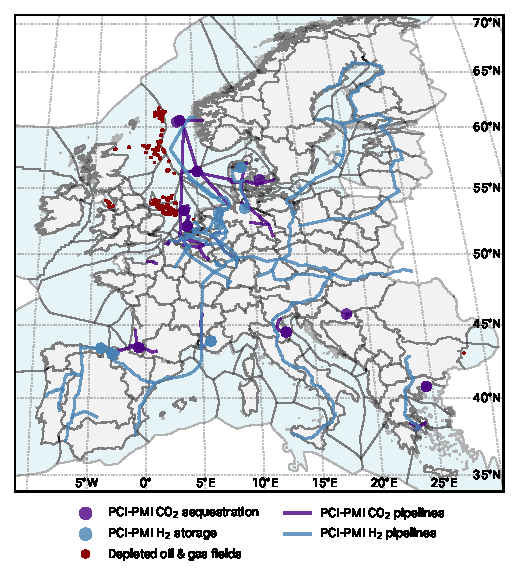
\includegraphics{map_adm_pcipmi}
  \caption{Map of the regional scope including clustered onshore (grey) and offshore regions (blue), as well as PCI-PMI \ce{CO2} and \ce{H2} pipelines, storage and sequestration sites. Depleted offshore oil and gas fields (red) provide additional \ce{CO2} sequestration potential \cite{hofmannH2CO2Network2025}.}
  \label{fig:regional_scope_map}
\end{figure}

Our implementation can adapt to the needs and configuration of the model, including selected technologies, geographical and temporal resolution, as well as considered sectors. Within this study, all projects are mapped to the 99 NUTS regions. In the mapping process, pipelines are aggregated and connect all regions that they are overpassing. Similar to how all electricity lines and carrier links are modelled in PyPSA-Eur, lengths are calculated using the haversine formula multiplied by a factor of 1.25 to account for the non-straight shape of pipelines.
We apply standardised cost assumptions \cite{zeyenPyPSATechnologydataV01012025} across all existing brownfield assets, exogenously specified PCI-PMI projects, and projects endogenously selected by the model, equally. Our approach is motivated by two considerations: (i) cost data submitted by project promoters are often incomplete and may differ in terms of included components, underlying assumptions, and risk margins; and (ii) applying uniform cost assumptions ensures comparability and a level playing field across all potential investments, including both PCI-PMI projects and endogenous model decisions.

\paragraph{\ce{CO2} sequestration and \ce{H2} storage sites}
\label{sec:co2_sequestration_sites}
Beyond \ce{CO2} sequestration site projects included in the latest PCI-PMI list (around 114 Mt p.a.), we consider additional technical potential from the European \ce{CO2} storage database \cite{europeancommissionEuropeanCO2Storage2020,hofmannH2CO2Network2025}. The dataset includes storage potential from depleted oil and gas fields and saline aquifers. While social and commercial acceptance of \ce{CO2} storage has been increasing in recent years, concerns still exist regarding its long-term role and safety \cite{vanalphenSocietalAcceptanceCarbon2007}.
We only consider conservative estimates from depleted oil and gas fields, which are primarily located offshore in the British, Norwegian, and Dutch North Sea (see Figure \ref{fig:regional_scope_map}), yielding a technical sequestration potential of \SI{7164}{Mt}. Our focus is motivated by the following reasons: (i) infrastructure such as wells, platforms, and pipelines already exist for depleted oil and gas fields and can be repurposed, significantly lowering costs and project risk; (ii) depleted fields are generally better understood geologically and have demonstrated sealing capacities, further reducing uncertainty; and (iii) repurposing former production sites is often more publicly and politically acceptable than developing entirely new storage locations, entirely. In contrast, while saline aquifers represent a substantial share of the total technical potential, they carry higher development costs and risks and are less likely to be advanced without strong policy and financial support \cite{europeancommissionEuropeanCO2Storage2020}. Note that the PCI-PMI project list includes some aquifer-based sequestration projects, however, their inclusion as PCI-PMI project indicates a higher likelihood of development.

We distribute the technical sequestration potential of the depleted oil and gas fields over a lifetime of 25 years (cf. \cite{hofmannH2CO2Network2025}), yielding an annual sequestration potential of up to 286 Mt p.a. We then cluster all offshore potential within a buffer radius of \SI{50}{km} per offshore bus region in each modelled NUTS region and connect them through offshore \ce{CO2} pipelines to the closest onshore bus. 

The model also includes \ce{H2} storage sites from the PCI-PMI list and allows for endogenous build-out of additional storage capacities by repurposing salt caverns \cite{neumannPotentialRoleHydrogen2023}.

\subsection{Scenario setup and regret matrix}
\label{sec:scenario_setup}
To assess the long-term impact of PCI-PMI projects on the European energy system and EU energy policies, we implement a regret matrix based approach. This allows us to evaluate the following questions: (i) What additional costs are incurred/saved by relaxed policy ambitions, delayed or cancelled PCI-PMI projects? (ii) What are alternative investment strategies to react to these events? 
\subsubsection{Long-term scenarios}
\paragraph{Scenario definition}
\label{sec:definition}
We define the long-term scenarios based on the degree of \ce{CO2} and \ce{H2} infrastructure build-out, including the roll-out of PCI-PMI projects as well additional pipeline investments. In total, we implement five long-term scenarios, (i) a pessimistic scenario (Decentral Islands --- \textit{DI}) without any \ce{H2} pipeline and onshore \ce{CO2} pipeline infrastructure, (ii) a scenario that considers the on-time commissioning of all PCI-PMI \ce{CO2} and \ce{H2} projects (PCI-PMI --- \textit{PCI}) only, (iii) more ambitious scenarios that further allow investments into national and (iv) international pipelines (PCI-PMI nat. --- \textit{PCI-n} and PCI-PMI internat. --- \textit{PCI-in}), and (v) a scenario that does not assume any fixed PCI-PMI infrastructure but allows for a centralised, purely needs-based build-out of \ce{CO2} and \ce{H2} pipelines (Centralised Planning --- \textit{CP}). An overview of the long-term scenarios and their associated model-endogenous decision variables is provided in Table \ref{tab:long-term_scenarios}. 

\begin{table}[htpb]
  \centering
  \caption{Overview of long-term scenarios and their key assumptions.}
  \label{tab:long-term_scenarios}
  \scriptsize
  \begin{tabularx}{\linewidth}{R{2.6cm}>{\centering\arraybackslash}X>{\centering\arraybackslash}X>{\centering\arraybackslash}X>{\centering\arraybackslash}X>{\centering\arraybackslash}X}
    \toprule
    \textbf{Long-term scenarios} & 
    \textbf{DI} & 
    \textbf{PCI} & 
    \textbf{PCI-n} & 
    \textbf{PCI-in} & 
    \textbf{CP} \\
    \midrule
    \textbf{\ce{CO2} sequestration} & & & & & \\
    Depleted oil \& gas fields* & $\blacksquare$ & $\blacksquare$ & $\blacksquare$ & $\blacksquare$ & $\blacksquare$ \\
    PCI-PMI seq. sites** & -- & $\blacksquare$ & $\blacksquare$ & $\blacksquare$ & $\blacksquare$ \\
    \midrule
    \textbf{\ce{H2} storage} & & & & & \\
    Endogenous build-out & $\blacksquare$ & $\blacksquare$ & $\blacksquare$ & $\blacksquare$ & $\blacksquare$ \\
    PCI-PMI storage sites & -- & $\blacksquare$ & $\blacksquare$ & $\blacksquare$ & $\blacksquare$ \\
    \midrule
    \textbf{\ce{CO2} pipelines} & & & & & \\
    to depleted oil \& gas fields & $\blacksquare$ & $\blacksquare$ & $\blacksquare$ & $\blacksquare$ & $\blacksquare$ \\
    to PCI-PMI seq. sites & -- & $\blacksquare$ & $\blacksquare$ & $\blacksquare$ & $\blacksquare$ \\
    \midrule
    \textbf{\ce{CO2} and \ce{H2} pipelines} & & & & & \\
    PCI-PMI & -- & $\blacksquare$ & $\blacksquare$ & $\blacksquare$ & $\blacksquare$ \\
    National build-out & -- & $\blacksquare$ & $\blacksquare$ & $\blacksquare$ & $\blacksquare$ \\
    International build-out & -- & -- & -- & $\blacksquare$ & $\blacksquare$ \\
    PCI-PMI extendable & -- & -- & -- & -- & $\blacksquare$ \\

    \bottomrule
  \end{tabularx}
  \caption*{\scriptsize $\blacksquare$ enabled \quad -- disabled \quad * approx. 286 Mt p.a. \quad ** approx. 114 Mt p.a.}
\end{table}

\paragraph{Targets}
\label{sec:targets}
In all long-term scenarios, emission, technology, sequestration and production targets have to be met for each planning horizon (see Table \ref{tab:targets}). For the year 2030, these targets are directly derived from the EU's policy targets, including a \SI{55}{\percent} reduction in greenhouse gas emissions compared to 1990 levels \cite{europeancommissionFit55Delivering2021}, \SI{10}{Mt} p.a. of domestic green \ce{H2} production \cite{europeancommissionREPowerEUPlanCommunication2022} and \SI{40}{GW} of electrolyser capacity \cite{europeancommissionCommunicationCommissionEuropean2020}, and \SI{50}{Mt} p.a. of \ce{CO2} sequestration capacity \cite{europeanparliamentRegulationEU20242024}. For 2050, the \ce{CO2} are based on the modelling the impact assessment for the EU's 2040 climate targets, in 250 Mt p.a. need to be sequestered \cite{europeancommissionCommunicationCommissionEuropean2024}. \ce{H2} production targets for 2050 are based on the European Commission's `METIS 3 study S5' \cite{europeancommission.directorategeneralforenergy.METIS3Study2023}, modelling possible pathways for industry decarbonisation until 2040. For 2040, we interpolate linearly between the 2030 and 2050 targets. The electrolyser capacities for 2040 and 2050 are scaled by the ratio of \ce{H2} production to electrolyser capacity in 2030. An overview of the targets and their values is provided in Table \ref{tab:targets}. We implement the green hydrogen production target as a minimum production constraint on electrolysis. Accordingly, we refer to this hydrogen as `electrolytic \ce{H2}' throughout this paper. Note that this implementation is based on an aggregated annual target without temporal matching rules.

\begin{table}[htbp]
  \centering
  \caption{Pathway for implemented targets.}
  \label{tab:targets}
  \scriptsize
  \begin{tabularx}{\linewidth}{R{2.6cm}>{\centering\arraybackslash}X>{\centering\arraybackslash}X>{\centering\arraybackslash}X}
    \toprule
    \textbf{Planning horizon} & \textbf{2030} & \textbf{2040} & \textbf{2050} \\
    \midrule
    \textbf{Targets} & & & \\
    GHG emission reduction &  \SI{-55}{\percent} & \SI{-90}{\percent} & \SI{-100}{\percent} \\
    \ce{CO2} sequestration & 50 Mt p.a. & 150 Mt p.a. & 250 Mt p.a. \\
    Electrolytic \ce{H2} production & 10 Mt p.a. & 27.5 Mt p.a. & 45 Mt p.a. \\
    \ce{H2} electrolyser capacity & \SI{40}{GW} &  \SI{110}{GW} &  \SI{180}{GW} \\
    \bottomrule
  \end{tabularx}
  \caption*{\scriptsize Climate and energy policy targets based on \cite{europeancommissionFit55Delivering2021,europeancommissionREPowerEUPlanCommunication2022,europeanparliamentRegulationEU20242024,europeancommissionCommunicationCommissionEuropean2024,europeancommission.directorategeneralforenergy.METIS3Study2023}}
\end{table}

\subsubsection{Short-term scenarios}
\label{sec:short-term_scenarios}
In a subsequent step, we examine the impact of various short-term scenarios on the long-term decarbonisation pathways. Specifically, we assume that the \ce{CO2} and \ce{H2} pipeline capacities identified in the long-term modelling exercise are either maintained at their planned levels, delayed in implementation, or not built at all.
In these short-term scenarios, the model can still react by investing into additional generation, storage, or conversion, or carbon-removal technologies, assuming the technical potential was not exceeded in the long-term optimisation. At this step, we also simulate changes in energy policy. For example, in \textit{Reduced targets}, we remove all of the long-term targets (Table \ref{tab:targets}) except for the GHG emission reduction targets to assess the value of the \ce{CO2} and \ce{H2} infrastructure in a less ambitious policy environment \cite{europeancourtofauditorsEUsIndustrialPolicy2024}. In \textit{Delayed pipelines}, we assume that all PCI-PMI and endogenous pipelines are delayed by one period, i.e., the commissioning of the project is shifted to the next planning horizon. Lastly, we remove all pipeline capacities in \textit{No pipelines}, including the PCI-PMI projects, allowing us to evaluate the impact of a complete lack of planned infrastructure. 

\begin{table}[t]
  \centering
  \caption{Regret matrix setup: Long-term and short-term scenarios.}
  \label{tab:regret_matrix_setup}
  \scriptsize
  \begin{tabularx}{\linewidth}{R{2.8cm}>{\centering\arraybackslash}X>{\centering\arraybackslash}X>{\centering\arraybackslash}X}
    \toprule
    \textbf{Short-term} & \textbf{Reduced targets} & \textbf{Delayed pipelines} & \textbf{No pipelines} \\
    \midrule
    \textbf{Long-term scenarios} & & & \\
    Decentral Islands (\textbf{DI}) & $\blacksquare$ & -- & -- \\
    PCI-PMI (\textbf{PCI}) & $\blacksquare$ & $\blacksquare$ & $\blacksquare$ \\
    PCI-PMI nat. (\textbf{PCI-n}) & $\blacksquare$ & $\blacksquare$ & $\blacksquare$\\
    PCI-PMI internat. (\textbf{PCI-in}) & $\blacksquare$ & $\blacksquare$ & $\blacksquare$ \\
    Central Planning (\textbf{CP}) & $\blacksquare$ & $\blacksquare$ & $\blacksquare$ \\
    \midrule
    \textbf{Targets} & & & \\
    GHG emission reduction &  $\blacksquare$ &  $\blacksquare$ &  $\blacksquare$ \\
    \ce{CO2} sequestration &  -- &  $\blacksquare$ &  $\blacksquare$ \\
    Electrolytic \ce{H2} production &  -- &  $\blacksquare$ &  $\blacksquare$ \\
    \ce{H2} electrolysers &  -- &  $\blacksquare$ &  $\blacksquare$ \\
    \midrule
    \textbf{\ce{CO2} + \ce{H2} infrastructure} & & & \\
    \ce{CO2} sequestration sites & $\blacksquare$ &  $\blacksquare$ &  $\blacksquare$ \\
    \ce{CO2} pipelines to seq. site & $\blacksquare$ &  $\blacksquare$ &  $\blacksquare$ \\
    \ce{CO2} pipelines & $\blacksquare$ &  $\square$ &  -- \\
    \ce{H2} pipelines & $\blacksquare$ &  $\square$ &  -- \\
    \bottomrule
  \end{tabularx}
  \caption*{\scriptsize $\blacksquare$ enabled \quad $\square$ delayed by one period \quad -- disabled}
\end{table}

Table \ref{tab:regret_matrix_setup} gives an overview of the regret matrix setup and its underlying assumptions, where the long-term scenario serves as the \textit{planned} or \textit{anticipated} and the short-term scenario serves as the hypothetically \textit{realised} outcome. A regret matrix provides a decision-making framework that evaluates the potential loss (\textit{regret}) associated with choosing one strategy over the other by comparing the outcomes, i.e., the total system costs. Here, the regret is quantified as the difference between system costs of the short-term scenario and the long-term (anticipated) scenario for each scenario. 
In total, we run 60 optimisations on a cluster: ($n_{LT} \times n_{planning\,horizons}) \times (1+n_{ST}) = 60$. Each calculation requires up to 160 GB of RAM and 8 to 16 hours to solve. The linear optimisation problems are solved using Gurobi.

\section{Results and discussion}
\label{sec:results_and_discussion}
We structure the results and discussion into three main sections. First, we present the results of the long-term scenarios. Then, we look at the impact of the short-term scenarios on the long-term scenarios, by comparing the economic regret and impacts on \ce{CO2} and \ce{H2} balances. Finally, we assess the benefits of the PCI-PMI projects with regard to reduced system costs and discuss the implications of our findings for the European energy system and its policy targets. 

\subsection{Long-term scenarios}
\label{sec:long-term_scenarios}
Figure \ref{fig:costs_overview} shows the total annual system costs --- distributed over all modelled technology groups --- for each planning horizon and long-term scenario. We observe the highest total annual system costs in the planning horizon 2040, ranging from \euro{912} to \euro{968} billion per year. This cost increase is primarily driven by the sharp decarbonisation pathway planned for 2030 to 2040 --- a carbon budget reduction of more than 1600 Mt p.a. compared to the remaining 460 Mt p.a. in the last decade from 2040 to 2050. In 2030, total system costs are lowest in the \textit{DI} and \textit{CP} scenario, as the model does not see the need for large-scale investments into \ce{H2} and \ce{CO2} infrastructure yet (due to myopic foresight). Adding PCI-PMI projects in 2030 increases costs by less than \SI{1}{\percent} (Figure \ref{fig:costs_overview}). With \ce{CO2} pipelines connecting depleted offshore oil and gas fields to their closest onshore region, the policy targets, including \ce{CO2} sequestration can be achieved at a total of \euro{865} billion per year.

\begin{figure}[t]
  \centering
  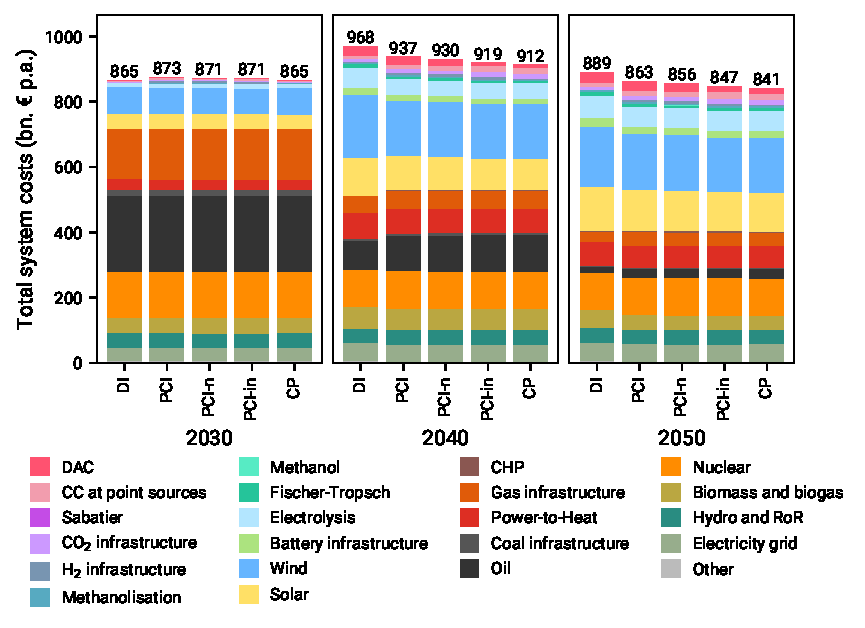
\includegraphics{costs_overview.pdf}
  \caption{Total annual system costs (CAPEX + OPEX) by technology group. \textit{\ce{CO2} and \ce{H2} infrastructure each include pipelines, storage and sequestration sites, respectively. Gas refers to gas power plants and boilers. Coal infrastructure refers to hard coal and lignite power plants. Other includes SMR, rural heat, and thermal storage.}}
  \label{fig:costs_overview}
\end{figure}

Starting in 2040, all scenarios with PCI-PMI and endogenous pipeline investments unlock significant cost savings, from more than \euro{30} billion per year in the \textit{PCI} up to \euro{50} billion per year in the \textit{PCI-in} scenario. 
By granting the model complete flexibility to expand hydrogen and \ce{CO2} infrastructure at any location beyond the PCI-PMI projects, we unlock additional annual cost savings of \euro{6} to \euro{7} billion per year through investments in fewer, yet more optimally located \ce{CO2} and \ce{H2} pipelines from a systemic perspective (see \textit{PCI-in} pipeline utilisation in Figure \ref{fig:PCI-in_lt} compared to \textit{CP} pipeline utilisation in Figure \ref{fig:CP_lt}).
Further, this reduces the reliance on larger investments into wind generation and costly DAC technologies near the sequestration sites. These effects are slightly less pronounced in the 2050 model results, where system costs can be reduced by \euro{26} to \euro{41} billion per year with PCI-PMI and endogenous pipeline investments. Here, higher carbon capture and utilisation (CCU) via methanol synthesis and Fischer-Tropsch processes, supported by increased \ce{H2} production as a chemical feedstock, enhances system flexibility compared to 2040 (Figures \ref{fig:balances_overview_co2_stored} and \ref{fig:balances_overview_H2}).

\begin{figure}[htbp]
  \centering
  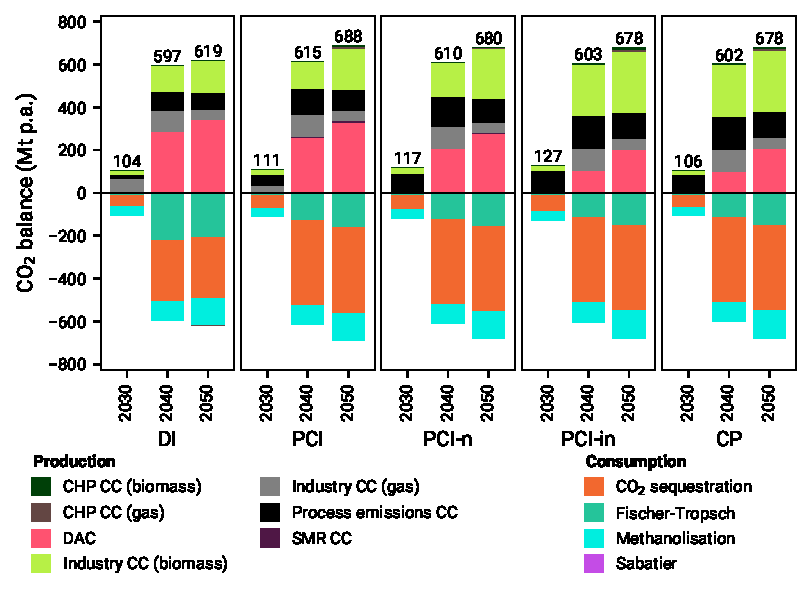
\includegraphics{balances_overview_co2 stored}
  \caption{\ce{CO2} balances in long-term scenarios.}
  \label{fig:balances_overview_co2_stored}
\end{figure}

\paragraph{CCUS}
\label{sec:ccus}
We find that most of the differences in system cost and savings can be attributed to the production and utilisation of \ce{CO2}, as shown in Figure \ref{fig:balances_overview_co2_stored}. Lacking the option to transport \ce{CO2} from industry and other point sources to the offshore sequestration sites, the system requires expensive DAC in the \textit{DI} scenario. While the sequestration target of 50 Mt p.a. in 2030 is binding only in the \textit{DI} scenario, all other scenarios achieve higher levels of \ce{CO2} sequestration as their \ce{CO2} pipeline build-out increases. 
The 53.9 Mt p.a. of \ce{CO2} sequestered in the \textit{CP} scenario serves as an indicator of the cost-optimal level of sequestration for the European energy system in 2030 assuming perfectly located pipeline infrastructure. With the inclusion of PCI-PMI projects, \ce{CO2} sequestration ranges from 58.7 Mt p.a. in the \textit{PCI} to 75 Mt p.a. in the \textit{PCI-in} scenario. 
Looking at 2040 and 2050, in place of expensive DAC in the \textit{DI} scenario, the model equips biomass-based industrial processes --- primarily located in Belgium, the Netherlands and Western regions of Germany --- with carbon capture (see Figures \ref{fig:PCI_lt_2030_co2}, \ref{fig:PCI_lt_2040_co2}, and \ref{fig:PCI_lt_2050_co2}). 

In 2040 and 2050, all sequestration targets (Table \ref{tab:targets}) are overachieved, as the full combined \ce{CO2} sequestration potential of 398 Mt p.a. is exploited in all scenarios where PCI-PMI projects are included (\textit{PCI} to \textit{CP}). 
Emissions are captured from industrial processes equipped with carbon capture units, with biomass-based industry contributing the largest share of point-source carbon capture. This ranges from 119 to 241 Mt p.a. in 2040 and from 149 to 287 Mt p.a. in 2050, increasing with the build-out of \ce{CO2} infrastructure (from left to right; see Figure 3). As the most expensive carbon capture option, \ce{CO2} capture from SMR CC processes is limited to a maximum of 8 Mt p.a. in the \textit{PCI} scenario by 2050.
With a lower sequestration potential of 286 Mt p.a. in \textit{DI} scenario, more \ce{CO2} is used as a precursor for the synthesis of Fischer-Tropsch fuels instead --- 221 Mt p.a. vs. 115-127 Mt p.a. in 2040 and 206 Mt p.a. vs. 153-163 Mt p.a. in 2050, to meet the emission reduction targets for 2040 and 2050, respectively. 
Given the fixed exogenous demand for shipping methanol (Figure \ref{fig:exogenous_demand}), \ce{CO2} demand for methanolisation is constant across all scenarios (39 Mt p.a. in 2030, 89 Mt p.a. in 2040, and 127 Mt p.a. in 2050). 

\paragraph{Hydrogen production and utilisation}
\label{sec:h2_production_and_utilisation}
\ce{H2} production in the model is primarily driven by the demand for Fischer-Tropsch fuels and methanol. In 2030 and 2050, the electrolytic \ce{H2} production target of 10 and 45 Mt p.a. is binding, equivalent to 333 and 1500 TWh p.a. (at a lower heating value of \SI{33.33}{kWh/kg} for \ce{H2}). Only in 2040, the \ce{H2} production target of 27.5 Mt p.a. (917 TWh p.a.) is overachieved by 185-247 TWh p.a. in the \textit{PCI} to \textit{CP} scenarios. \ce{H2} production in the \textit{DI} is significantly higher, given its need for additional Fischer-Tropsch synthesis to bind \ce{CO2} as an alternative to sequestration, as described in the previous section.
In 2050, Fischer-Tropsch fuels are primarily used to satisfy the demand for kerosene in aviation and naphta for industrial processes (see Table \ref{fig:exogenous_demand}). Only about 93 to 173 TWh p.a. of hydrogen is directly used in the industrial sector. Across all long-term scenarios, hydrogen is almost exclusively produced via electrolysis. Note that the model includes a green hydrogen production constraint reflecting energy policy targets, though it does not enforce an hourly matching rule.
In the \textit{DI} scenario, where there is no hydrogen pipeline infrastructure, the model resorts to Steam Methane Reforming (SMR) to produce 71 to 102 TWh p.a. of hydrogen in 2040 and 2050, respectively.

\begin{figure}[t]
  \centering
  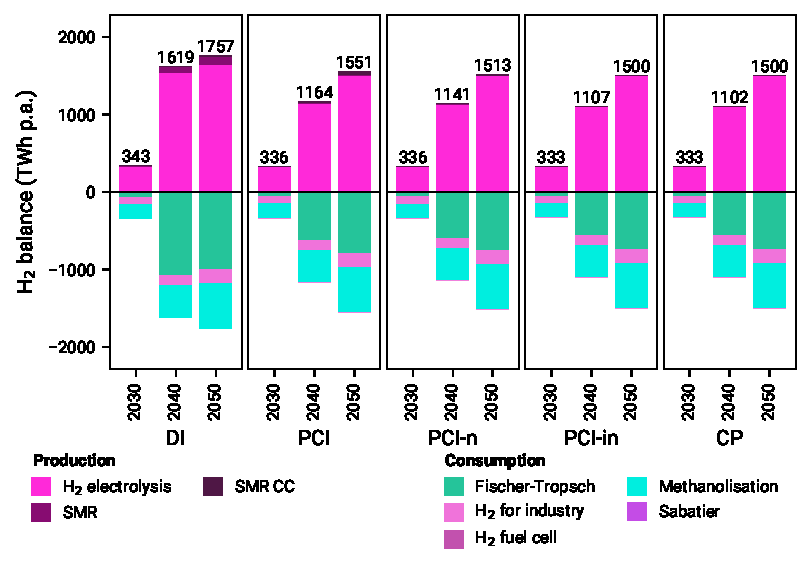
\includegraphics{balances_overview_H2}
  \caption{\ce{H2} balances in long-term scenarios.}
  \label{fig:balances_overview_H2}
\end{figure}

\begin{figure*}[htbp]
  \centering
  \begin{subfigure}[t]{0.33\textwidth}
      \vspace{0pt}
      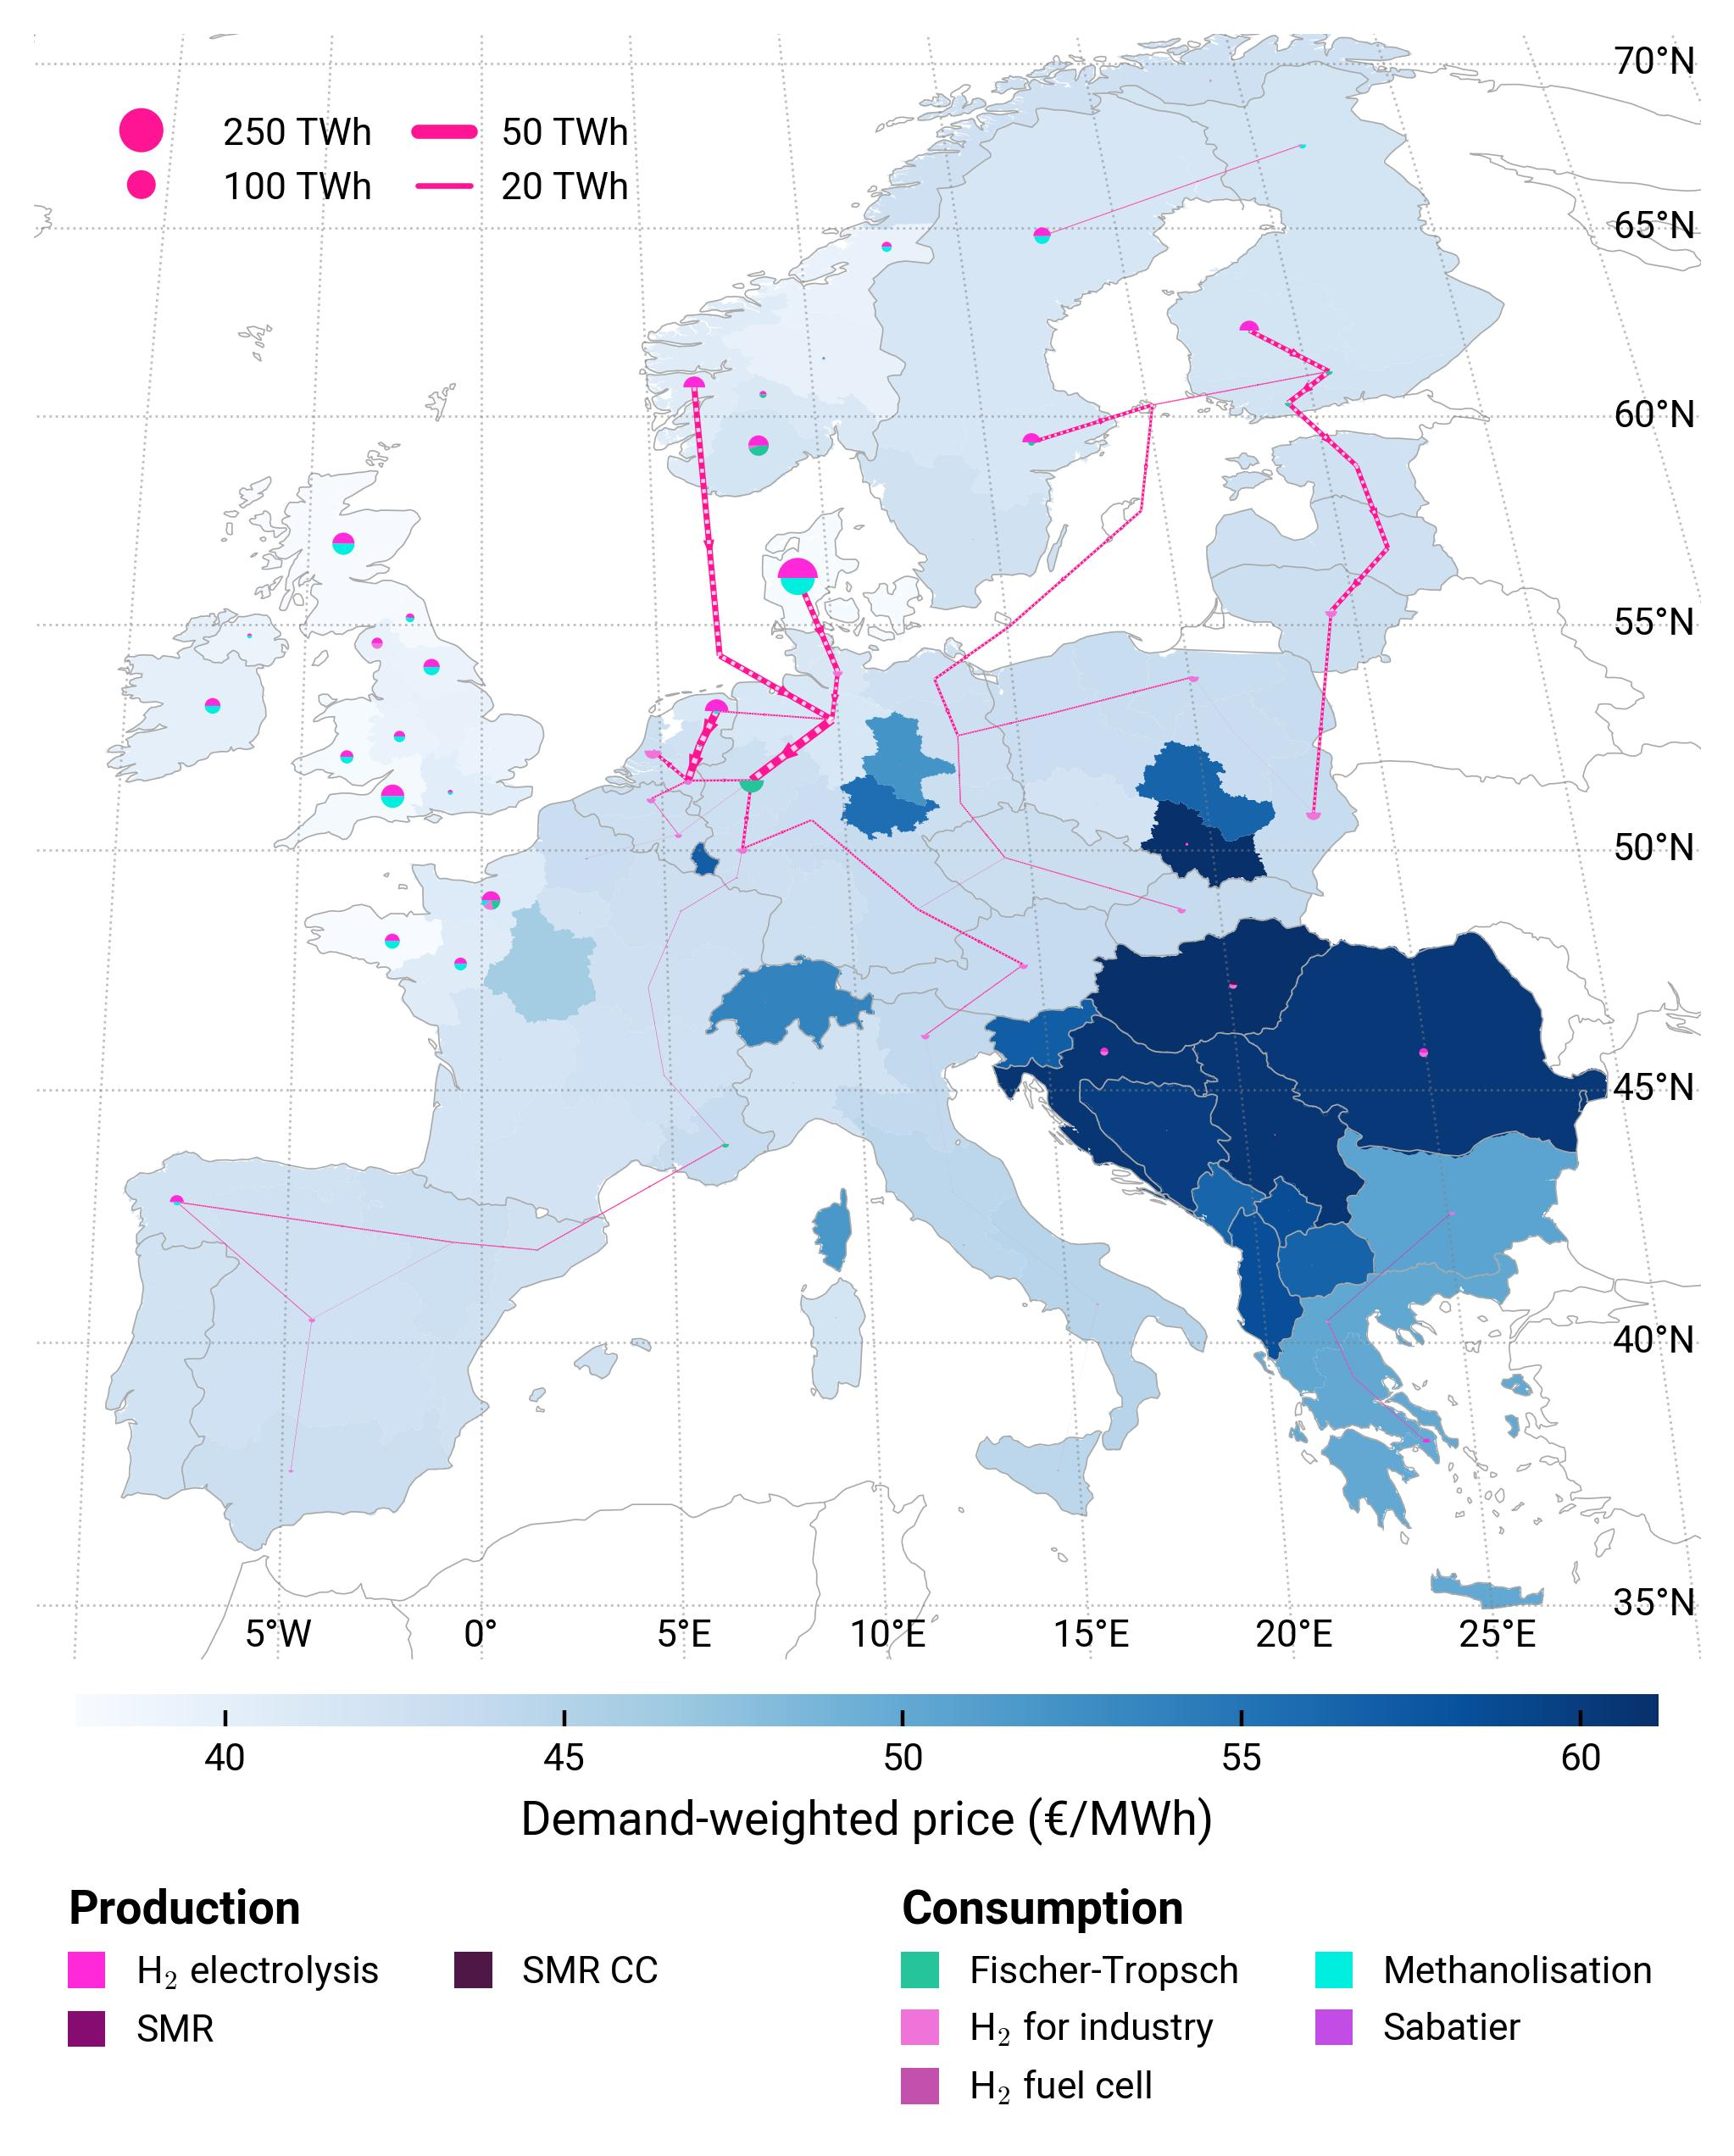
\includegraphics[width=1\textwidth]{maps/pcipmi/base_s_adm___2030-balance_map_H2}
      \caption{\ce{H2} 2030.}
      \label{fig:PCI_lt_2030_h2}
  \end{subfigure}
  \begin{subfigure}[t]{0.33\textwidth}
      \vspace{0pt}
      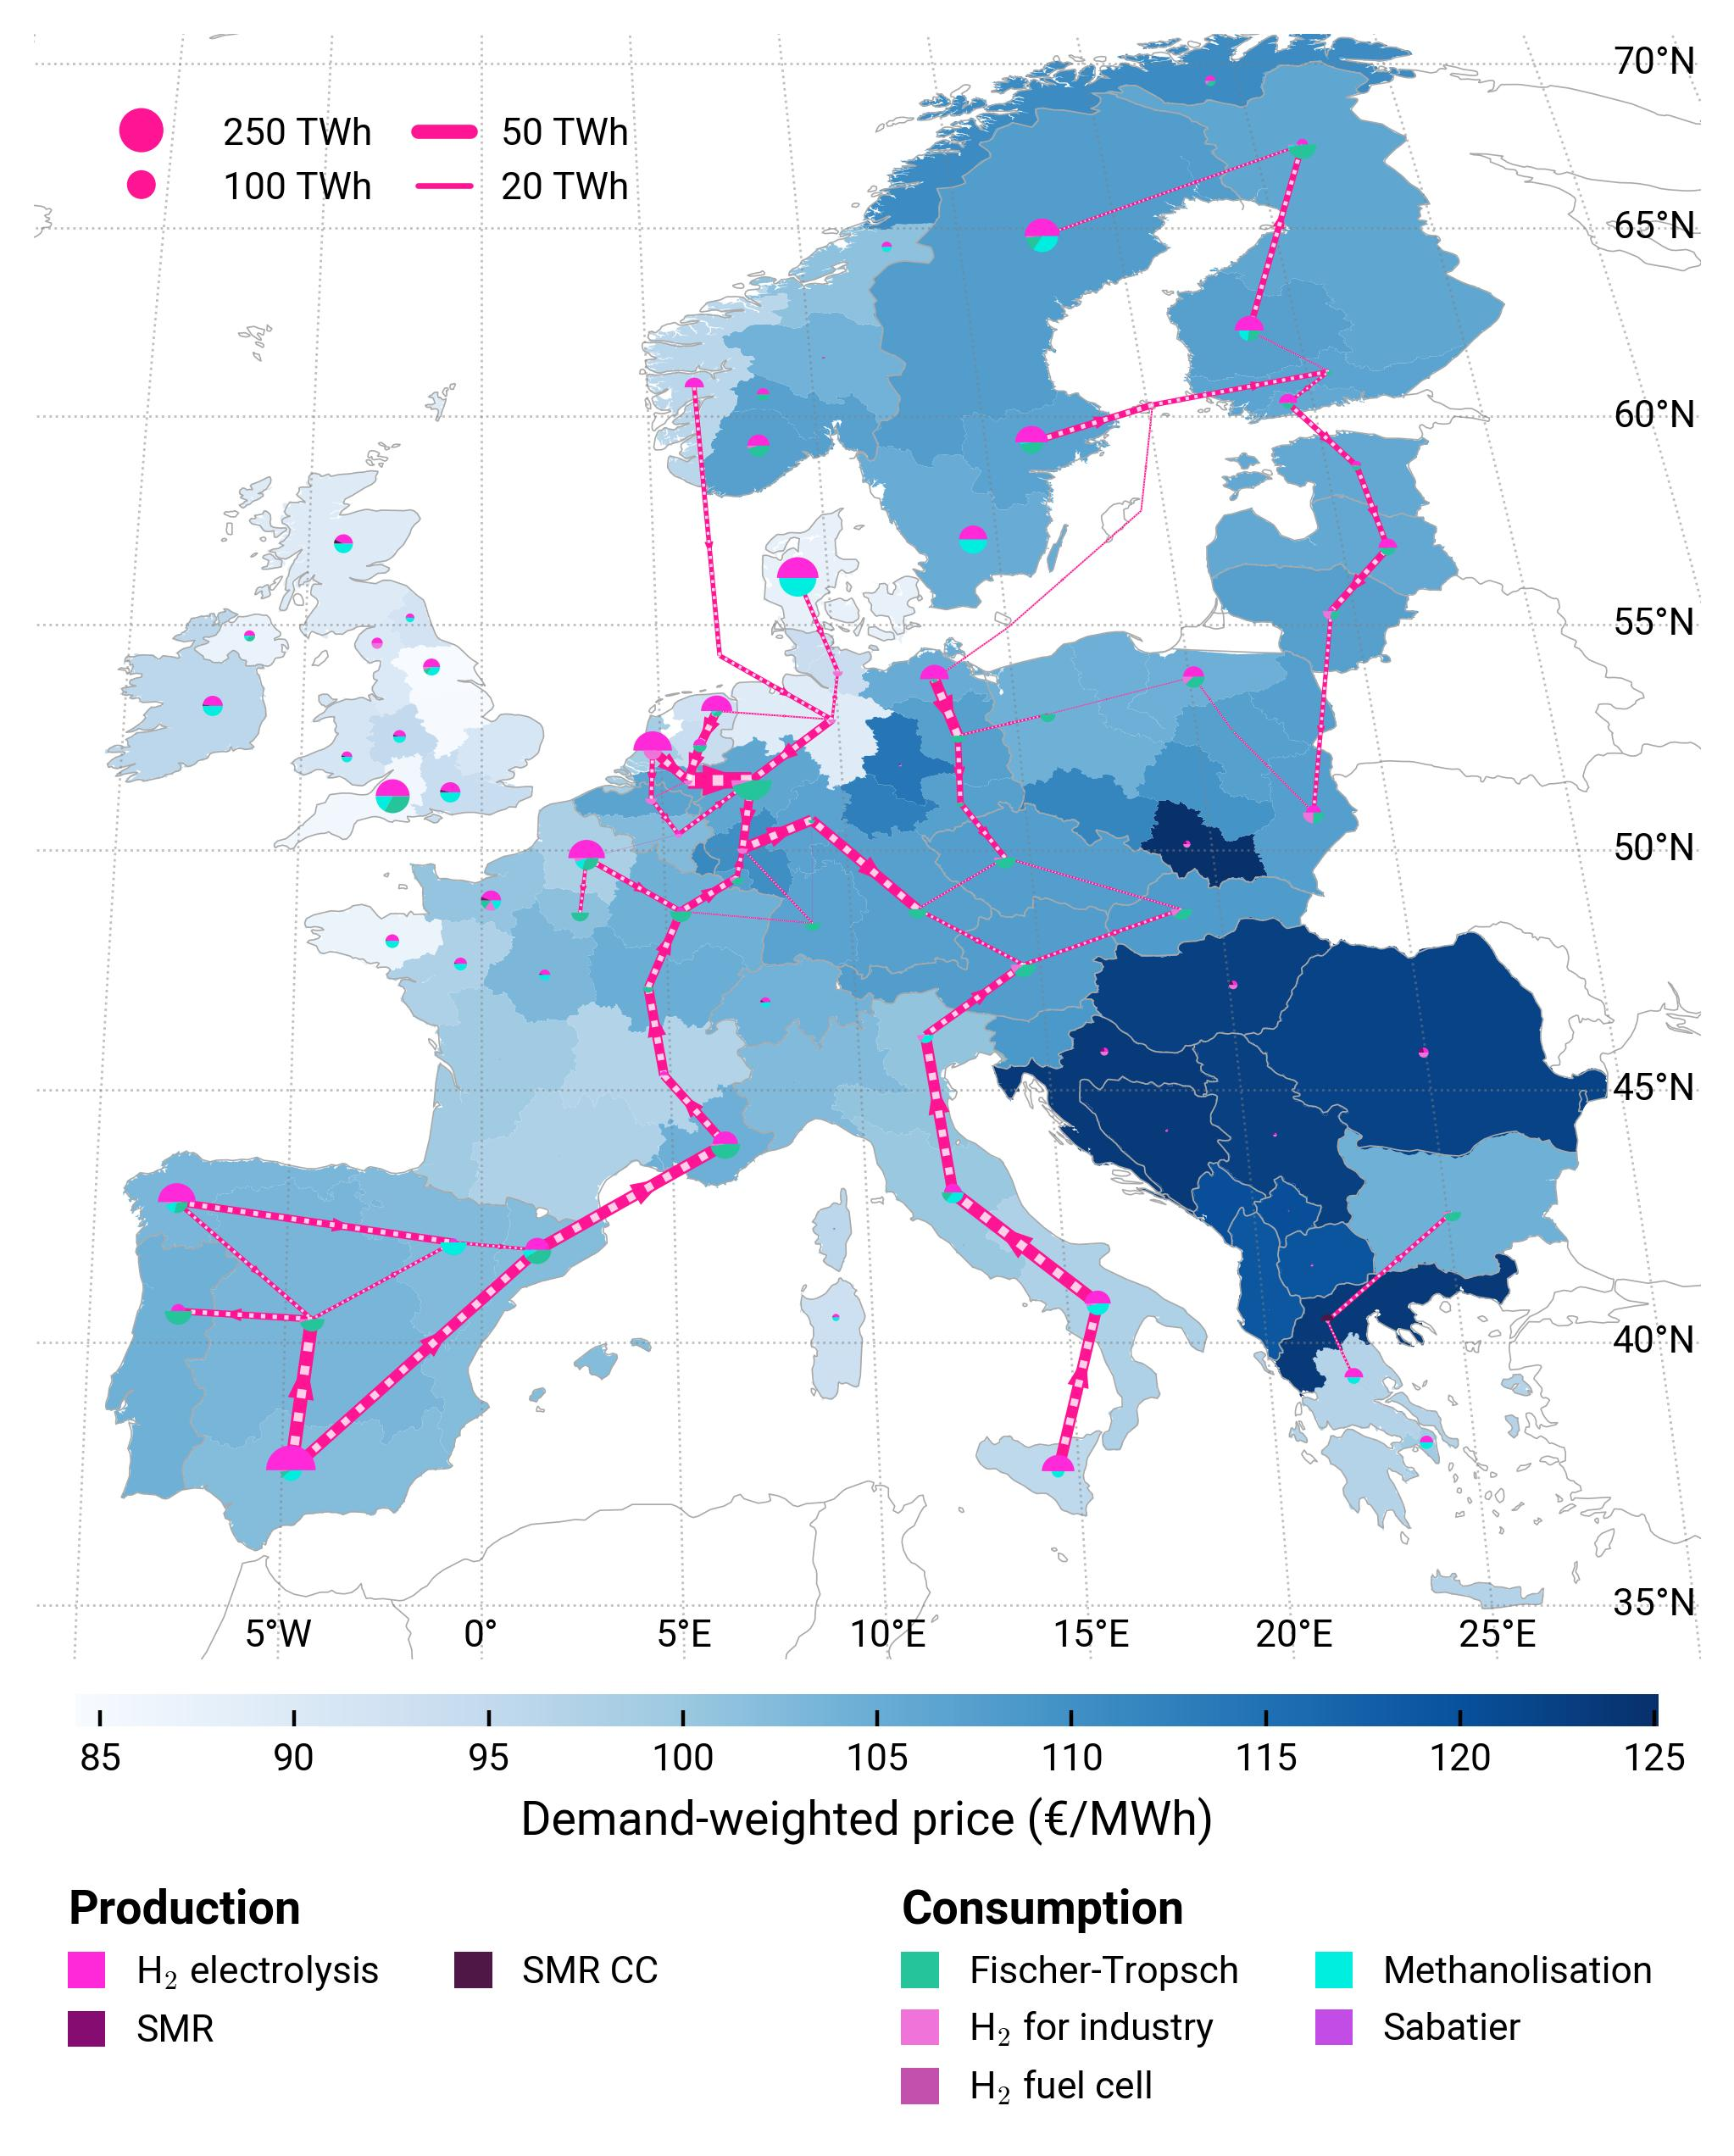
\includegraphics[width=1\textwidth]{maps/pcipmi/base_s_adm___2040-balance_map_H2}
      \caption{\ce{H2} 2040.}
      \label{fig:PCI_lt_2040_h2}
  \end{subfigure}
  \begin{subfigure}[t]{0.33\textwidth}
    \vspace{0pt}
    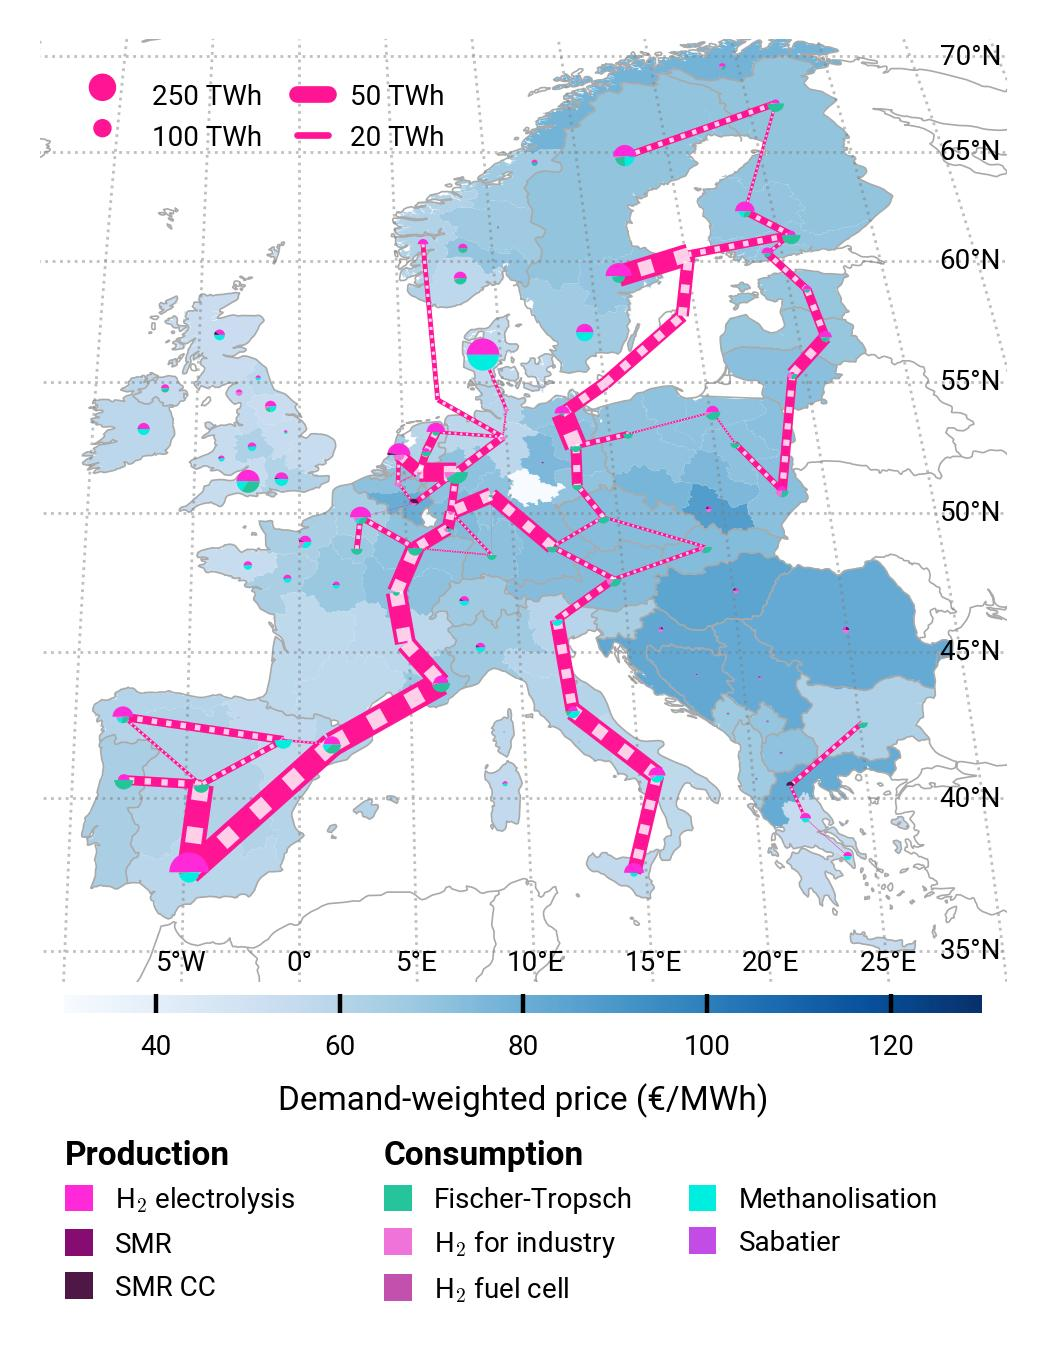
\includegraphics[width=1\textwidth]{maps/pcipmi/base_s_adm___2050-balance_map_H2}
    \caption{\ce{H2} 2050.}
    \label{fig:PCI_lt_2050_h2}
  \end{subfigure}
  \begin{subfigure}[t]{0.33\textwidth}
      \vspace{0pt}
      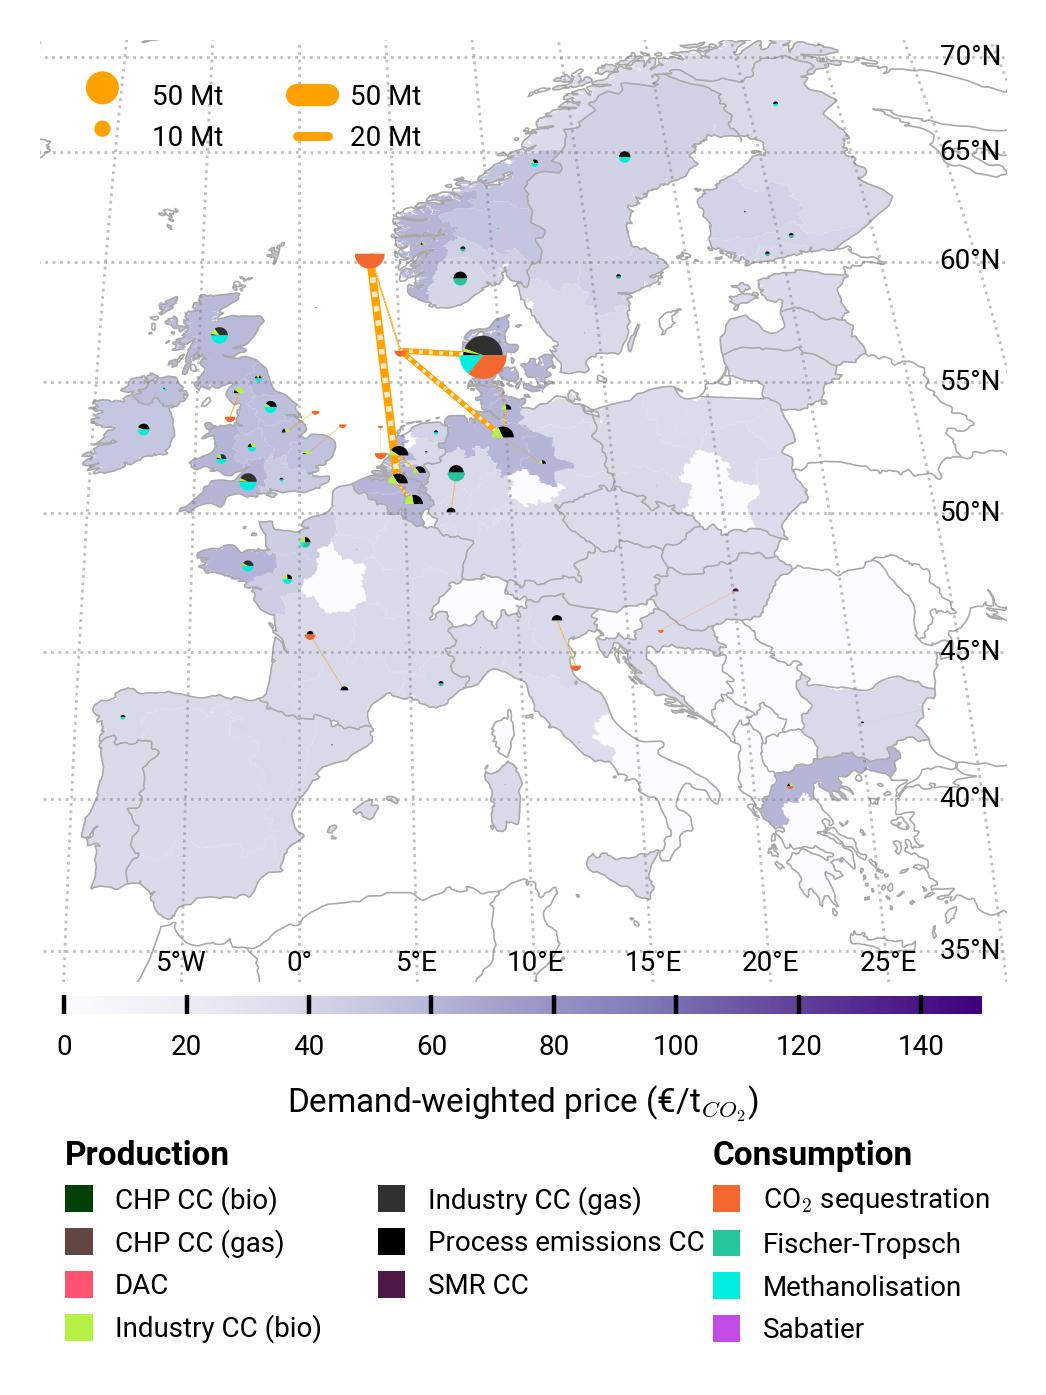
\includegraphics[width=1\textwidth]{maps/pcipmi/base_s_adm___2030-balance_map_co2_stored} 
      \caption{\ce{CO2} 2030.}
      \label{fig:PCI_lt_2030_co2}
  \end{subfigure}
  \begin{subfigure}[t]{0.33\textwidth}
      \vspace{0pt}
      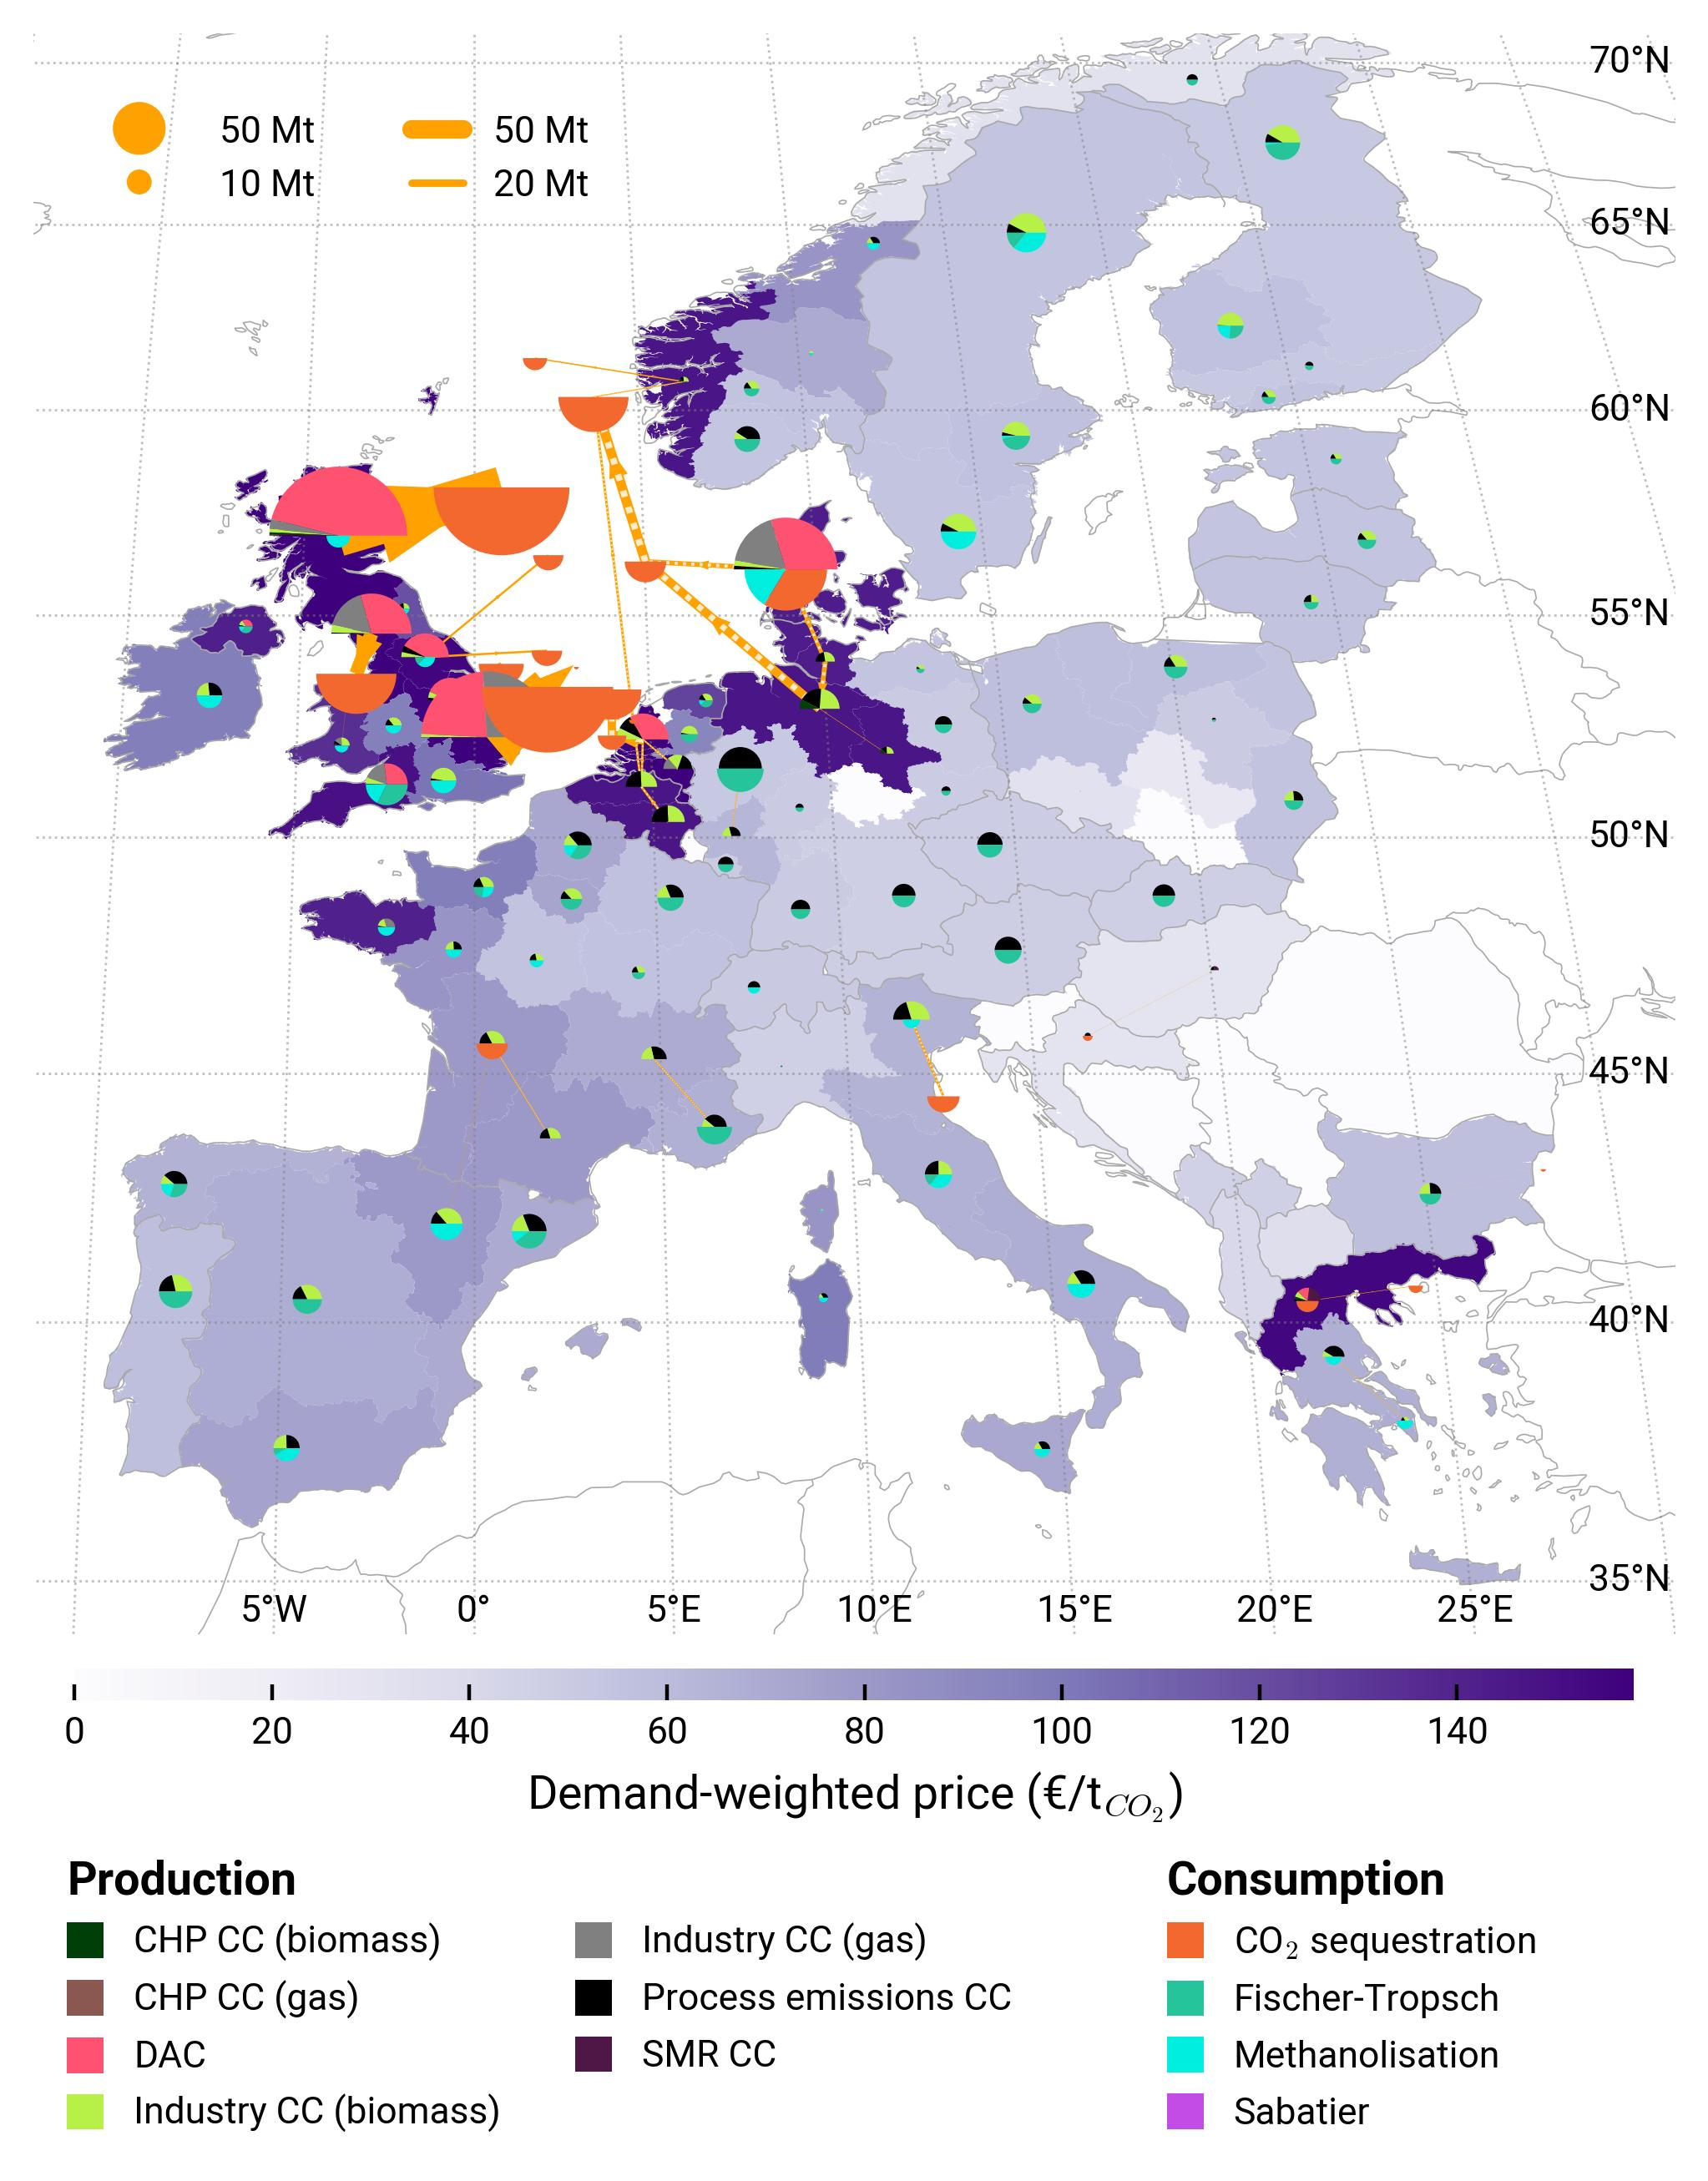
\includegraphics[width=1\textwidth]{maps/pcipmi/base_s_adm___2040-balance_map_co2_stored} 
      \caption{\ce{CO2} 2040.}
      \label{fig:PCI_lt_2040_co2}
  \end{subfigure}
  \begin{subfigure}[t]{0.33\textwidth}
      \vspace{0pt}
      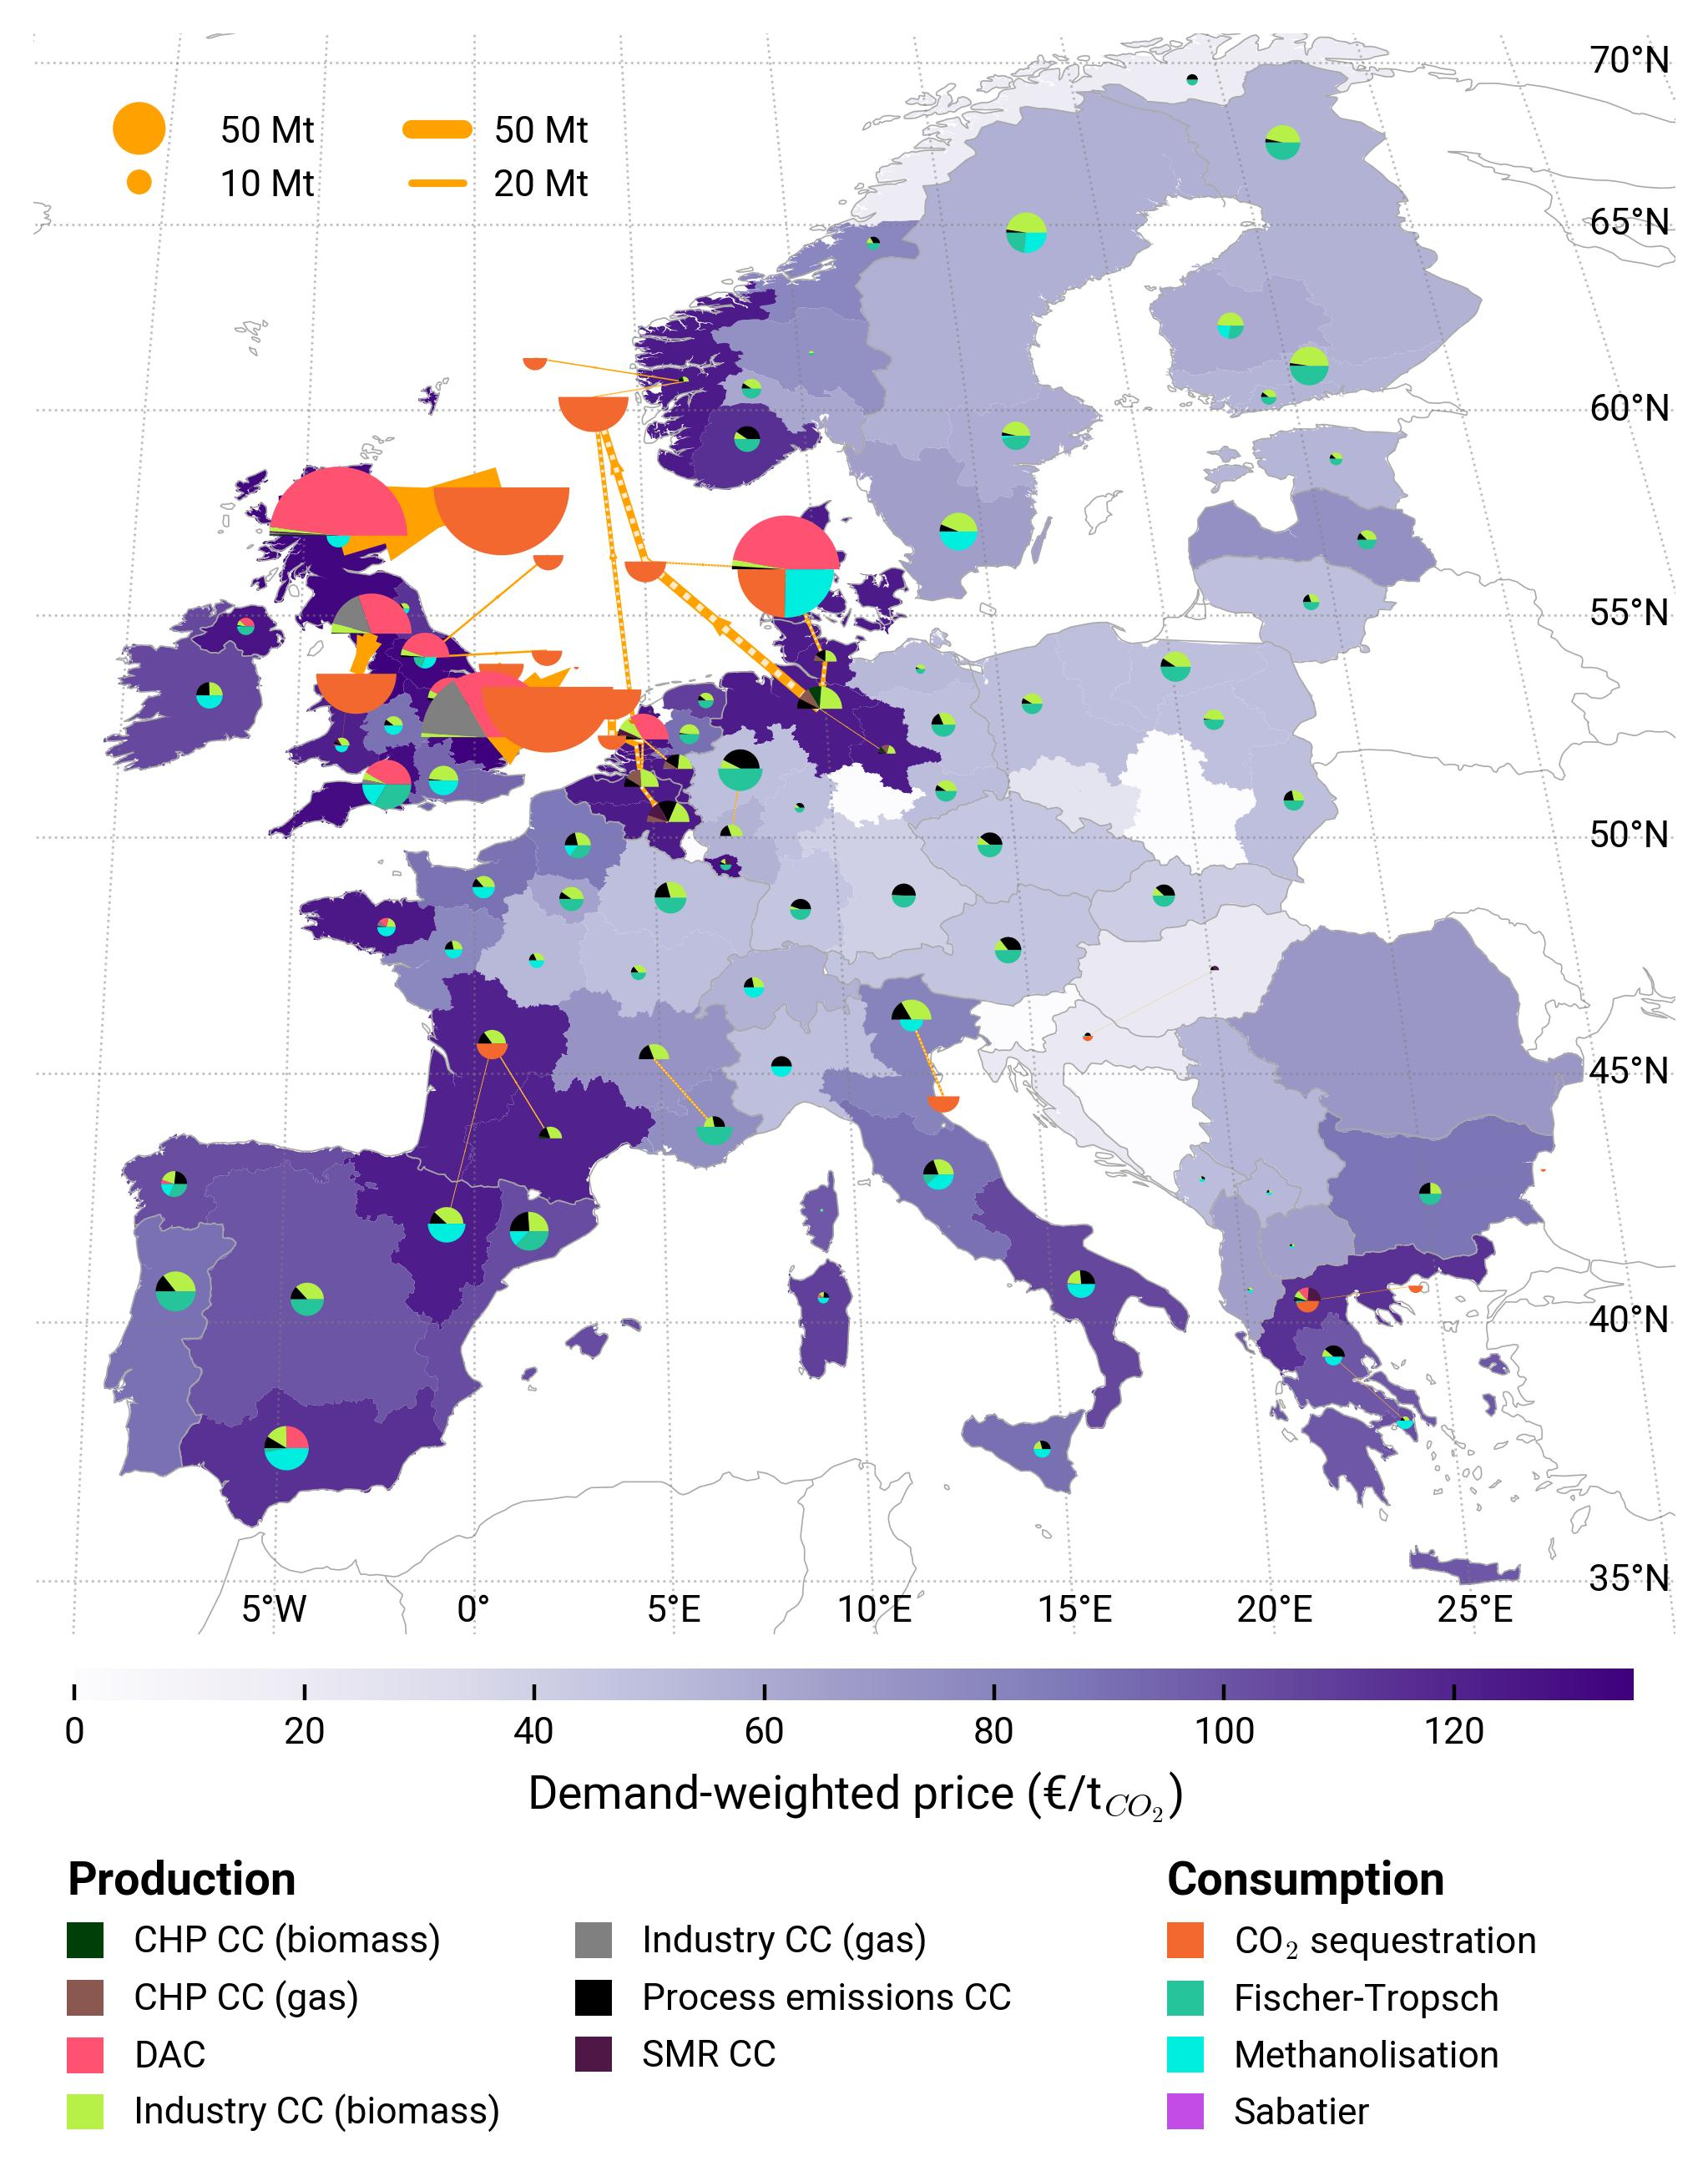
\includegraphics[width=1\textwidth]{maps/pcipmi/base_s_adm___2050-balance_map_co2_stored} 
      \caption{\ce{CO2} 2050.}
      \label{fig:PCI_lt_2050_co2}
  \end{subfigure}
  \vspace{0.3cm}
  \caption{\textit{PCI-PMI} long-term scenario --- Regional distribution of \ce{H2} and \ce{CO2} production, utilisation, storage, transport and price. \textit{Note that both the \ce{H2} and \ce{CO2} price refer to their value as a commodity, i.e., price is higher where there is a demand for it.}}
  \label{fig:PCI_lt}
\end{figure*}

Geographically, \ce{H2} production is concentrated in regions with high solar PV potential such as the Iberian and Italian Peninsula, as well as high wind infeed regions including Denmark, the Netherlands and Belgium. The produced \ce{H2} is then transported via \ce{H2} pipelines including PCI-PMI projects to carbon point sources  in central, continental Europe where it is used as a precursor for Fischer-Tropsch fuels. Onsite \ce{H2} production and consumption primarily occurs in conjunction with methanolisation processes. Figures \ref{fig:PCI_lt_2030_h2}, \ref{fig:PCI_lt_2040_h2}, and \ref{fig:PCI_lt_2050_h2} provide a map of the regional distribution of \ce{H2} production, utilisation, and transport in the \textit{PCI} scenario. Additional maps are provided in \ref{app:results}. Note that PCI-PMI projects or candidates (in \textit{CP} scenario) are plotted in dotted white lines.

\subsection{Regret analysis}
\label{sec:regret_analysis}

In this section, we discuss the impact of the three short-term scenarios described in Section \ref{sec:short-term_scenarios} on the long-term decarbonisation pathways, by comparing the economic regret, as well as the effects on \ce{CO2} utilisation, sequestration, and \ce{H2} production.
We calculate the regret terms by subtracting the annual total system costs of the long-term scenarios (row) from the short-term scenarios (columns). 
The values represent the additional costs incurred by a given short-term scenario relative to the benchmark. Positive values indicate higher costs, driven by increased investments in alternative generation, conversion, storage, and CDR technologies, as well as changes in their operation due to (i) delays or (ii) cancellations of pipeline infrastructure including PCI-PMI projects. Negative values indicate cost savings, which may arise under relaxed policy ambitions—for example, when \ce{CO2} and \ce{H2} targets are removed in the \textit{Reduced targets} scenario.


\begin{figure}[t]
  \centering
  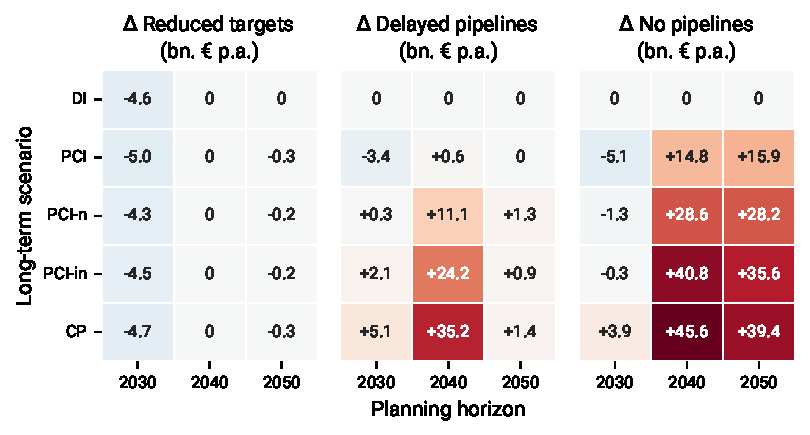
\includegraphics{regret_matrix}
  \caption{Regret matrix. \textit{Positive values indicate higher costs, driven by increased investments in alternative generation, conversion, storage, and CDR technologies, as well as changes in their operation due to (i) delays or (ii) cancellations of pipeline infrastructure including PCI-PMI projects. Negative values indicate cost savings, which may arise under relaxed policy ambitions—for example, when \ce{CO2} and \ce{H2} targets are removed in the \textit{Reduced targets} scenario.}}
  \label{fig:regret_matrix_results}
\end{figure}

Figure \ref{fig:regret_matrix_results} shows the regret matrix for all scenarios and planning horizons. From left to right, the first column shows the regret terms for the \textit{Reduced targets} scenario, where all long-term targets are removed except for the GHG emission reduction target. The second column shows the regret terms for the \textit{Delayed pipelines} scenario, where all PCI-PMI and endogenous pipelines are delayed by one period. The third column shows the regret terms for the \textit{No pipelines} scenario, where all hydrogen and \ce{CO2} pipeline capacities are removed.

In the \textit{Reduced targets} scenario, overall system costs change only marginally despite the relaxation of specific targets. This is because \ce{CO2} sequestration levels are primarily driven by the overarching GHG emission constraints --- particularly the stringent 2040 and 2050 carbon budgets, which remain in place. With regard to hydrogen, the long-term results have previously shown that \ce{H2} production targets were overachieved in 2040. Only in 2030, we see a net negative regret of around \euro{4.3} to \euro{4.6} billion per year, as the minimum \ce{H2} production target was binding in the long-term scenario. Across all long-term scenarios, we have observed that \ce{CO2}
 pipeline infrastructure is not essential in 2030 (see Figure \ref{fig:CP_lt_2030_co2}). In the case of \ce{H2} pipeline infrastructure, the solution appears relatively flat: regrets in the \textit{DI} scenario without any pipelines (Figure \ref{fig:DI_lt_2030_co2}) are nearly identical to those in the \textit{CP} scenario (Figure \ref{fig:CP_lt_2030_co2}) with substantial pipeline deployment. When the \ce{H2} production and \ce{CO2} sequestration targets are removed, pipelines become even less relevant, although the associated cost savings are minimal, ranging from \euro{4.3} to \euro{5} billion per year in 2030 and 2040.

For similar reasons, the 2030 results for the \textit{Delayed pipelines} and \textit{No pipelines} scenarios exhibit small regret terms. Cost savings of \euro{3.4} to \euro{5.1} billion per year in the \textit{PCI} scenario suggest that, for 2030, mandating PCI-PMI projects is neither cost- nor topologically optimal in the short term. In contrast, a regret of \euro{3.9} to \euro{5.1} billion per year in the \textit{CP} scenario indicates some dependency on the invested pipeline infrastructure (Figure \ref{fig:CP_lt}) which represents the systemically more optimised solution.

When looking at the more long-term perspective, we see significant regrets in the \textit{Delayed pipelines} and \textit{No pipelines} scenarios. Having originally planned the energy system layout (including generation, transport, conversion technologies and storage) in the long-term scenario with PCI-PMI projects and/or endogenous pipelines, the model has to find alternative investments to still meet all targets, as the pipelines now materialise one period later or not at all. Regrets peak in 2040, where a delay of pipelines costs the system between \euro{0.6} to \euro{24.2} billion per year. in the scenarios with PCI-PMI projects and up to \euro{35.2} billion p.a. in the \textit{CP} scenario. 2050 regrets are lower than 2040 regrets, as almost all PCI-PMI pipelines are originally commissioned by 2030. Hence, a delay of projects from 2040 to 2050 only mildly impa
cts the system costs by \euro{0.6} billion per year. The more pipelines invested beyond those of PCI-PMI projects, the higher the regret if they are delayed. In 2050, very few additional \ce{CO2} and \ce{H2} pipelines are built, as such, a delay only increases system costs by \euro{0.9} to \euro{1.4} billion per year. 
The short-term scenario \textit{No pipelines} shows the highest regrets, ranging from \euro{14.8} to \euro{45.6} billion per year in 2040 and \euro{15.9} to \euro{39.4} billion per year in 2050. Note that this scenario represents a hypothetical worst case, as it is highly unlikely to plan an energy system with pipeline investments in mind yet fail to implement any of them.

Consistently throughout all short-term scenarios, most of the additional cost stem from the need to invest into additional carbon capture, renewable generation, and conversion technologies (see Figure \ref{fig:capacities_overview_extended}). Additional renewable generation capacities are made up of solar PV and wind. A significant higher amount of electrolyser capacity of more than 50 GW is needed in 2040 if pipelines are delayed. 

\begin{figure}[htbp]
  \centering
  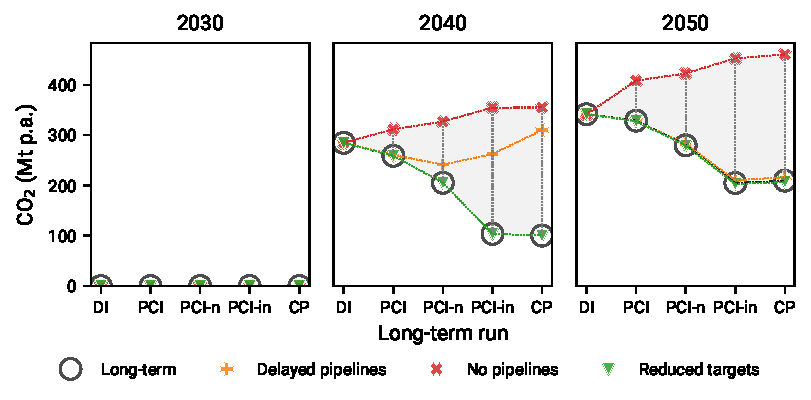
\includegraphics{delta_balances_DAC}
  \caption{Delta balances --- \ce{CO2} from DAC.}
  \label{fig:delta_balances_dac}
\end{figure}

\paragraph{Carbon capture}
Further, the model has to invest in more than 28 GW of carbon capture units at point sources and an additional 14 GW in DAC technologies to meet the sequestration and emission reduction targets. Cost-wise, the short-term investments into DAC technologies make up to a half of the of the additional system costs in both the \textit{Delayed pipelines} and \textit{No pipelines} scenarios (see Figure \ref{fig:costs_overview_extended}). DAC utilisation can increase from 40 Mt p.a. in the \textit{PCI-n} to more than 200 Mt p.a. in the \textit{CP} scenario when pipelines are delayed (see Figure \ref{fig:balances_overview_extended_co2_stored}). If pipelines are not built at all, additional 60 Mt p.a. in the \textit{PCI} up to 250 Mt p.a. in the \textit{CP} scenario are captured from DAC, substituting a large share of \ce{CO2} previously captured from point sources equipped with carbon capture (biomass-based industry processes and non-abatable process emissions).

Note that a clear trade-off between the reliance on pipeline infrastructure and the need for DAC technologies can be observed in Figure \ref{fig:delta_balances_dac}. While the reliance on DAC decreases with the build-out of pipeline infrastructure, the model in return has to invest in more DAC if pipelines are delayed or not built at all. There is a risk involved, that the need for DAC is even higher in the scenarios with pipeline infrastructure compared to the \textit{DI} scenario, especially in later years (2040 and 2050), if the pipelines do not materialise at all, seeing a potential increase of 50 Mt p.a. in 2040 and 80 Mt p.a. in 2050 in the \textit{PCI} scenario.
\paragraph{\ce{H2} production} 
We find that the electrolytic \ce{H2} production target of 10 Mt p.a. (333 TWh p.a.) in 2030 is overly ambitious. Figure \ref{fig:balances_overview_extended_H2_stored} shows that in the \textit{Reduced targets} scenario, 132 to 151 TWh p.a. of \ce{H2}, corresponding to almost half of the target is produced from SMR instead of electrolysis. When pipelines are delayed, the model has to fall back to more decentral \ce{H2} production of an additional 55 to 187 TWh p.a. of \ce{H2} from electrolysis, SMR and SMR with carbon capture (the latter being the most expensive option). In the \textit{No pipelines} scenario, this additional \ce{H2} production increases to up to 305 TWh p.a (see Figure \ref{fig:balances_overview_extended_H2_stored}).

\subsection{Value of PCI-PMI projects}
\label{sec:value_of_pcipmi_projects}
Looking at the long-run we find that PCI-PMI projects, while not completely cost-optimal compared to a centrally planned system, are still cost-beneficial. Compared to a complete lack of \ce{H2} and \ce{CO2} pipeline infrastructure as well as lower \ce{CO2} sequestration potential, the \textit{PCI} scenario unlocks annual cost savings in up to \euro{30.7} billion per year. Figure \ref{fig:totex_heatmap} shows the total system costs or Total Expenditures (TOTEX) p.a. split into Capital (CAPEX) and Operational Expenditures (OPEX) p.a., as well as the Net Present Value (NPV) of total system costs, discounted at an interest rate of \SI{7}{\percent} p.a.
Even when accounting for the additional costs of \euro{0.6} billion per year faced in the \textit{Delayed pipelines} and up to \euro{15.9} billion per year in the \textit{No pipelines} scenario, a net positive is achieved, indicating that investing into the PCI-PMI infrastructure is a no-regret option. By connecting further \ce{H2} production sites and \ce{CO2} point sources to the pipeline network. additional cost savings of up to \euro{18.4} billion per year can be achieved in the \textit{PCI-in} scenario. The \textit{CP} scenario serves as a theoretical benchmark, allowing the model to invest freely, not bound by \textit{forced} PCI-PMI projects. The model can invest in fewer, but more optimally located \ce{CO2} and \ce{H2} pipelines from a systemic perspective. Economic benefits of all pipeline investments materialise after 2030, yielding lower NPV of potentially at least \euro{75} billion over the course of the assets' lifetime. 

\begin{figure}[t]
  \centering
  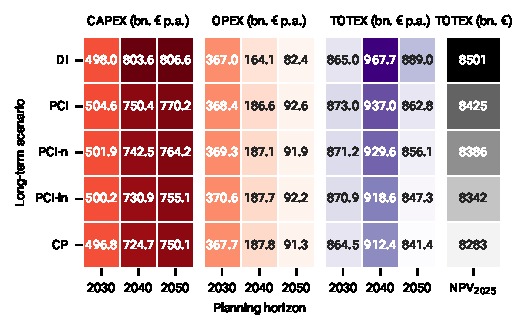
\includegraphics{totex_heatmap.pdf}
  \caption{Annual system costs by long-term scenario and planning horizon.}
  \label{fig:totex_heatmap}
\end{figure}

\subsection{Limitations of our study}
\label{sec:limitations}
While our study assesses a variety of topologies, planning horizons, and potential regret scenarios, it is not exhaustive and comes with limitations.
As we focus on the impact of continental European PCI-PMI infrastructure, we neglect fuel and energy imports from outside Europe. \ce{H2} and \ce{CO2} demand is directly driven by fixed, exogenous demands for the respective carrier or their derivatives.

Regarding the modelling of both \ce{H2} and \ce{CO2} pipelines, we assume a level playing field for all pipeline projects through standardised costs and applying haversine distance, i.e., no discrimination between PCI-PMI projects and other projects, this is a simplification as real costs may differ. We also do not discretise the endogenously built pipelines (due to computational complexity) and allow any capacity to be built. This assumption can lead to underestimation of the true costs of pipeline investments.

Further, all results are based on a single weather year, i.e., 2013.
Other limitations include geographic and temporal clustering to make the problem solving computationally feasible.
\section{Conclusion}
\label{sec:conclusion}

In this study, we have assessed the impact of PCI-PMI projects on reaching European climate targets on its path to net-zero by 2050. We have modelled the European energy system with a focus on \ce{H2} and \ce{CO2} infrastructure, and evaluated the performance of different levels of pipeline roll-out under three short-term scenarios. 


\paragraph{Economic viability and policy targets}
Our findings demonstrate that PCI-PMI \ce{CO2} and \ce{H2} infrastructure generate a net positive impact on total system costs, even when accounting for potential additional costs involved with the delay of pipelines. This positions PCI-PMI projects as a no-regret investment option for the European energy system, when treated as a whole.
Their economic benefit increases considerably when strategic pipeline extensions are implemented, connecting additional \ce{H2} production sites and \ce{CO2} point sources to the pipeline network. 
Compared to a system without any pipeline infrastructure, PCI-PMI projects help to achieve the EU's ambitious policy targets, including net-zero emissions, \ce{H2} production and \ce{CO2} sequestration targets, while reducing system costs and technology dependencies.

\paragraph{CCUS and hydrogen utilisation}
The pipeline infrastructure serves dual purposes in Europe's decarbonisation strategy: \ce{H2} pipelines facilitate the distribution of more affordable green \ce{H2} from northern and south-western regions rich in renewable energy potential to high-demand regions in central Europe. Complementarily, \ce{CO2} transport and offshore sequestration sites enable industrial decarbonisation by linking major industrial sites and their process emissions to offshore sequestration sites in the North Sea, particularly in Denmark, Norway, and the Netherlands.

\paragraph{Technology and risk diversification}
The build-out of \ce{CO2} and \ce{H2} pipeline infrastructure helps utilising renewable energy sources more efficiently. Hydrogen pipelines enable the transport of green \ce{H2} over long distances while \ce{CO2} pipelines reduce the reliance on single carbon capture technologies such as Direct Air Capture and point-source carbon capture, confirming the findings of \cite{hofmannH2CO2Network2025}. This diversification further enhances system resilience towards uncertainties involved with technologies that are not yet commercially available at scale, such as Direct Air Capture.

\paragraph{Political support and public acceptance} 
While PCI-PMI may not achieve perfect cost-optimality in their entirety compared to a theoretically centrally planned system, they possess benefits beyond pure economic viability. The success of large-scale infrastructure investments highly depend on continuous political support and public acceptance --- factors that are particularly favourable for PCI-PMI projects.
Backed directly by the European Commission, PCI-PMI projects benefit from stronger political endorsement, institutional support structures, enhanced access to financing and grants, and accelerated permitting processes. Additionally, the requirement for frequent and transparent progress reporting increases their likelihood of gaining public acceptance.

\section*{CRediT authorship contribution statement}
\textbf{Bobby Xiong}: Conceptualisation, Methodology, Software, Validation, Investigation, Data Curation, Writing --- Original Draft, Review \& Editing, Visualisation. \textbf{Iegor Riepin}: Conceptualisation, Methodology, Investigation, Writing --- Review \& Editing, Project Administration, Supervision. \textbf{Tom Brown}: Investigation, Resources, Writing --- Review \& Editing, Supervision, Funding acquisition.

\section*{Declaration of competing interest}
The authors declare that they have no known competing financial interests or personal relationships that could have appeared to influence the work reported in this paper.

\section*{Data and code availability}
All results, including solved PyPSA networks and summaries in .csv format are published on Zenodo: \newline
\href{https://doi.org/XX.YYYY/zenodo.10000000}{https://doi.org/XX.YYYY/zenodo.10000000}

The entire workflow, including the custom model based on PyPSA-Eur v2025.01.0, PCI-PMI project implementation, regret matrix setup, postprocessing and visualisation routines can be completely reproduced from the GitHub repository: \newline 
\href{https://github.com/bobbyxng/pcipmi-policy-targets}{https://github.com/bobbyxng/pcipmi-policy-targets}

\section*{Acknowledgements}
This work was supported by the German Federal Ministry for Economic Affairs and Climate Action (BMWK) under Grant No. 03EI4083A (RESILIENT). This project has been funded by partners of the CETPartnership (\href{https://cetpartnership.eu}{https://cetpartnership.eu}) through the Joint Call 2022. As such, this project has received funding from the European Union's Horizon Europe research and innovation programme under grant agreement no. 101069750.


%% The Appendices part is started with the command \appendix;
%% appendix sections are then done as normal sections
\appendix

\section{Data \& methodology}
\label{app:data_methodology}

\begin{figure}[htbp]
  \centering
  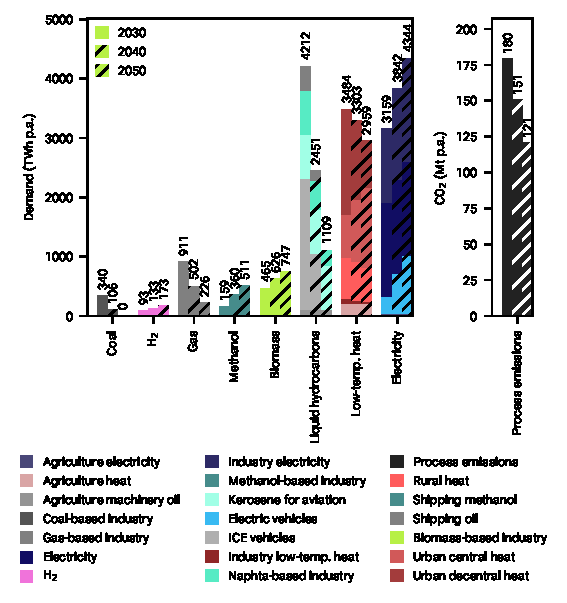
\includegraphics{exogenous_demand.pdf}
  \caption{Exogenous demand.}
  \label{fig:exogenous_demand}
\end{figure}

\begin{table}[htbp]
  \centering
  \caption{Cost assumptions for key technologies based on \cite{zeyenPyPSATechnologydataV01012025}.}
  \label{tab:cost_assumptions}
  \scriptsize
  \begin{tabularx}{\linewidth}{R{2.4cm}>{\centering\arraybackslash}X>{\centering\arraybackslash}X>
  {\centering\arraybackslash}X}
    \toprule
    & \textbf{Unit} & \textbf{CAPEX} & \textbf{FOM} \\
    \midrule
    \textbf{Pipeline infrastructure} & & & \\
    \ce{CO2} onshore pipelines & \euro{}/t\ce{CO2}/hkm & \num{2116} & \SI{0.9}{\percent/a} \\
    \ce{CO2} offshore pipelines & \euro{}/t\ce{CO2}/hkm & \num{4233} & \SI{0.5}{\percent/a} \\
    \ce{H2} onshore pipelines & \euro{}/MW$_{H_2}$/km & \num{304} & 1.5-\SI{3.2}{\percent/a} \\
    \ce{H2} offshore pipelines & \euro{}/MW$_{H_2}$/km & \num{456} & \SI{3.0}{\percent/a} \\
    \midrule
    \textbf{Conversion} & & & \\
    Electrolysis & \euro{}/kW$_e$ & \num{1000}-\num{1500} & \SI{4.0}{\percent/a} \\
    SMR & \euro{}/MW$_{CH_4}$ & \num{522201} & \SI{5.0}{\percent/a} \\
    SMR CC & \euro{}/MW$_{CH_4}$ & \num{605753} & \SI{5.0}{\percent/a} \\

    \bottomrule
  \end{tabularx}
\end{table}

\begin{table}[htbp]
  \centering
  \caption{Regional clustering: A total of 99 regions are modelled, excluding offshore buses.}
  \label{tab:regional_clustering}
  \scriptsize
  \begin{tabularx}{\linewidth}{R{2cm}>{\centering\arraybackslash}X>{\centering\arraybackslash}X}
    \toprule
     & \textbf{Country} & \textbf{Buses} \\
    \midrule
    \textbf{Admin. level} & $\bm\sum$ & \textbf{99} \\
    NUTS2 & Finland (FI) & 4 \\
          & Norway (NO) & 6 \\
    \midrule
    NUTS1 & Belgium (BE)** & 2 \\
          & Switzerland (CH) & 1 \\
          & Czech Republic (CZ) & 1 \\
          & Germany (DE)* & 13 \\
          & Denmark (DK) & 1 \\
          & Estonia (EE) & 1 \\
          & Spain (ES)* & 5 \\
          & France (FR) & 13 \\
          & Great Britain (GB)* & 11 \\
          & Greece (GR) & 3 \\
          & Ireland (IE) & 1 \\
          & Italy (IT)* & 6 \\
          & Lithuania (LT) & 1 \\
          & Luxembourg (LU) & 1 \\
          & Latvia (LV) & 1 \\
          & Montenegro (ME) & 1 \\
          & Macedonia (MK) & 1 \\
          & Netherlands (NL) & 4 \\
          & Poland (PL) & 7 \\
          & Portugal (PT) & 1 \\
          & Sweden (SE) & 3 \\
          & Slovenia (SI) & 1 \\
          & Slovakia (SK) & 1 \\
    \midrule
    NUTS0 & Albania (AL) & 1 \\
          & Austria (AT) & 1 \\
          & Bosnia and Herzegovina (BA) & 1 \\
          & Bulgaria (BG) & 1 \\
          & Croatia (HR) & 1 \\
          & Hungary (HU) & 1 \\
          & Romania (RO) & 1 \\
          & Serbia (RS) & 1 \\
          & Kosovo (XK) & 1 \\
    \bottomrule
  \end{tabularx}
  \caption*{\scriptsize City-states (*) (i.e., Berlin, Bremen, Hamburg, Madrid, and London) and regions without substations (**) (one in BE) are merged with neighbours. Sardinia and Sicily are modelled as two separate regions.}
\end{table}

\newpage
\section{Results}
\label{app:results}
\begin{figure}[htbp]
  \centering
  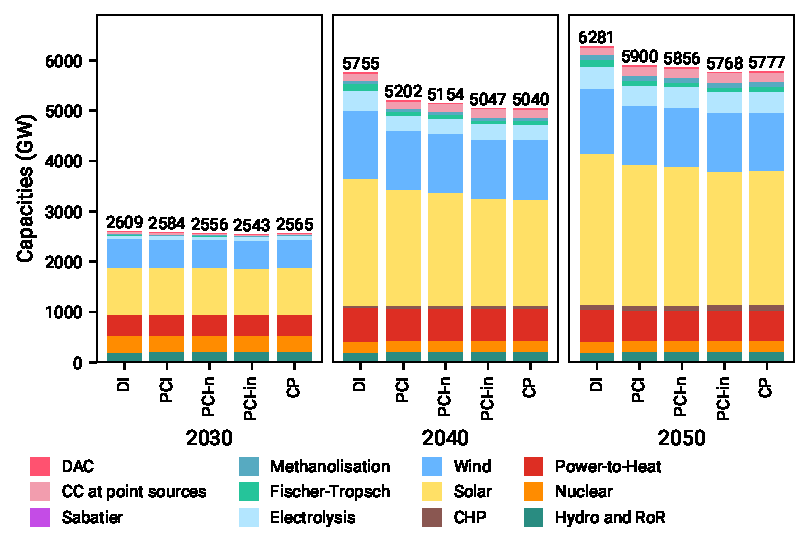
\includegraphics{capacities_overview.pdf}
  \caption{Installed capacities in long-term scenarios.}
  \label{fig:capacities_overview}
\end{figure}

\begin{figure}[htbp]
  \centering
  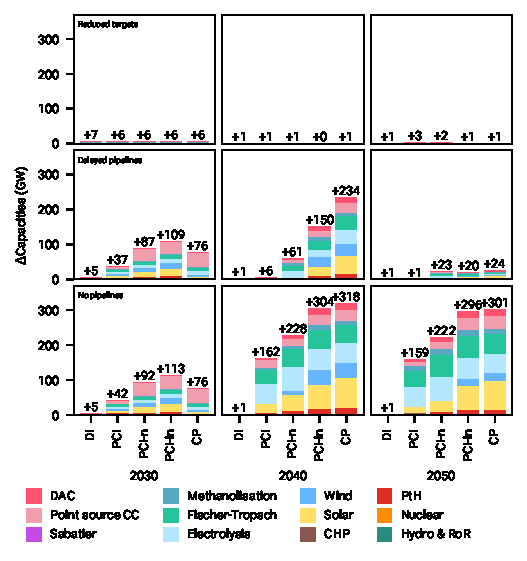
\includegraphics{capacities_overview_extended.pdf}
  \caption{$\Delta$Capacities --- Short-term minus long-term runs.}
  \label{fig:capacities_overview_extended}
\end{figure}

\begin{figure}[htbp]
  \centering
  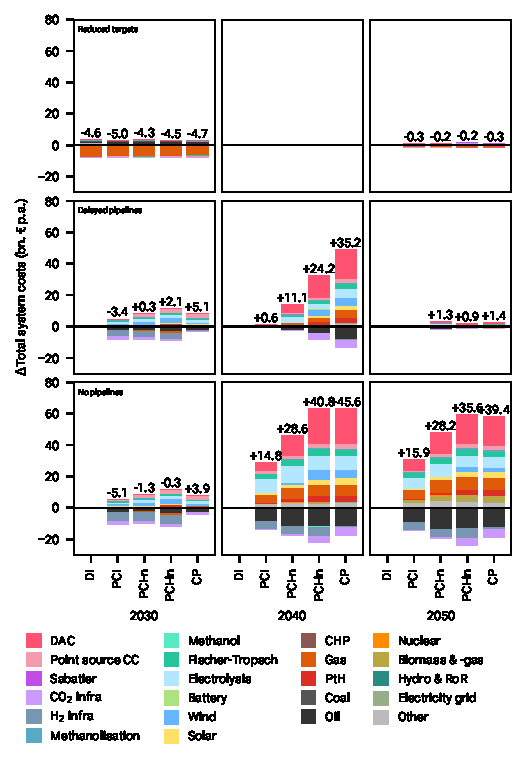
\includegraphics{costs_overview_extended.pdf}
  \caption{$\Delta$System costs --- Short-term minus long-term runs.}
  \label{fig:costs_overview_extended}
\end{figure}
\begin{figure}[htbp]
  \centering
  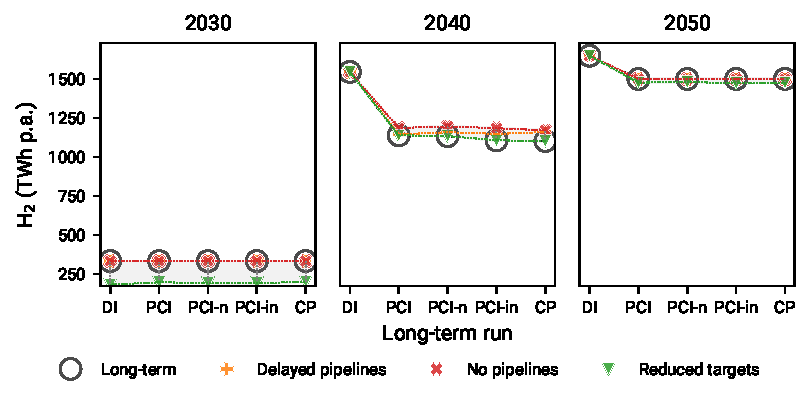
\includegraphics{delta_balances_H2 Electrolysis}
  \caption{Delta balances --- Electrolytic \ce{H2} production}
  \label{fig:delta_balances_h2_electrolysis}
\end{figure}
\begin{figure}[htbp]
  \centering
  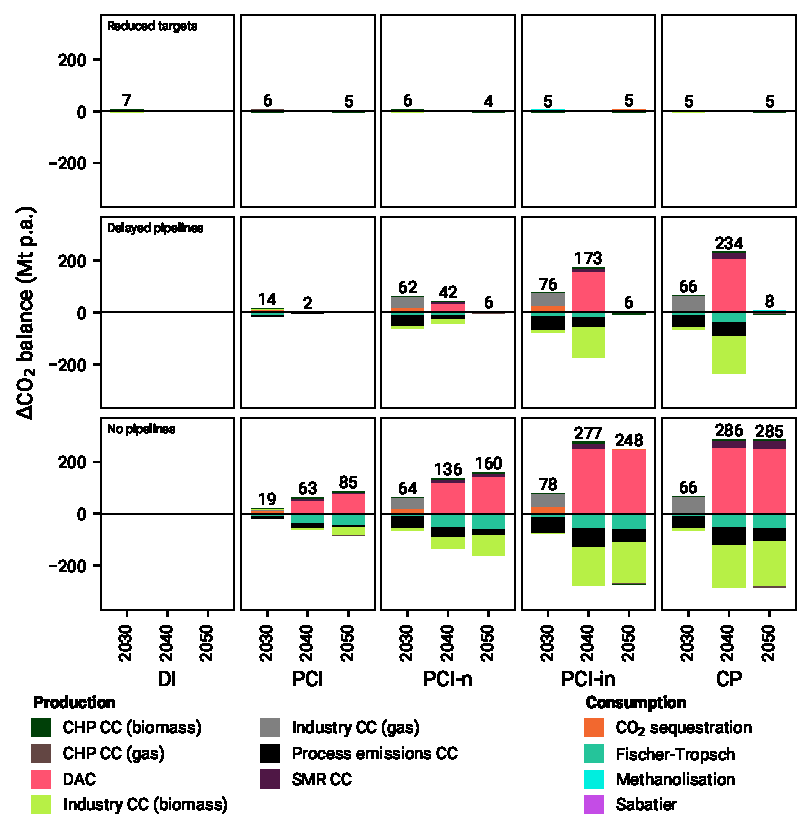
\includegraphics[width=\linewidth]{balances_overview_extended_co2 stored}
  \caption{$\Delta$\ce{CO2} balances --- Short-term minus long-term runs.}
  \label{fig:balances_overview_extended_co2_stored}
\end{figure}

\begin{figure}[htbp]
  \centering
  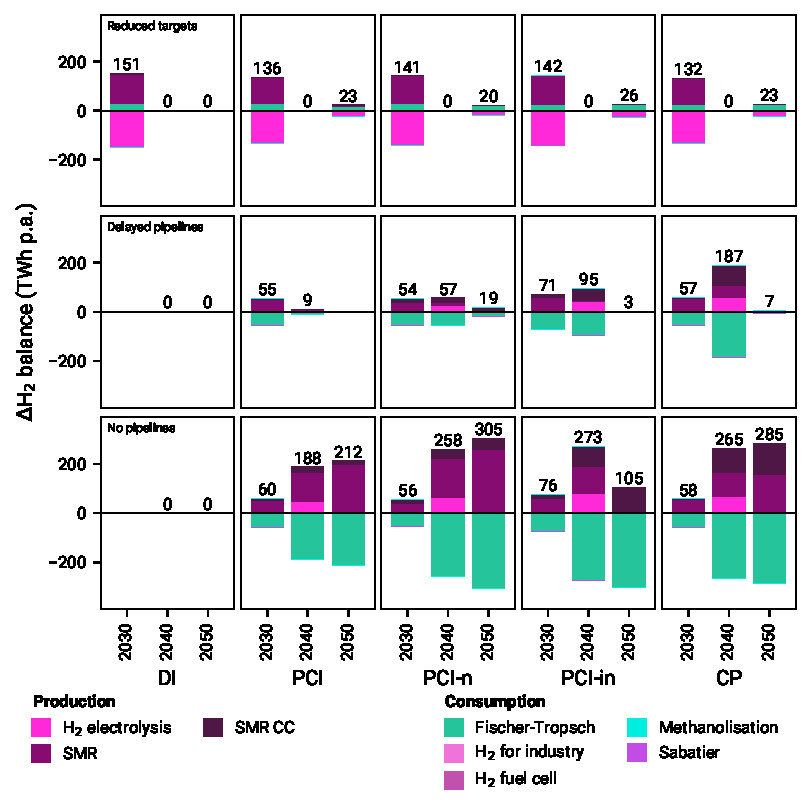
\includegraphics[width=\linewidth]{balances_overview_extended_H2}
  \caption{$\Delta$\ce{H2} balances --- Short-term minus long-term runs.}
  \label{fig:balances_overview_extended_H2_stored}
\end{figure}

\begin{figure}[htbp]
  \centering
  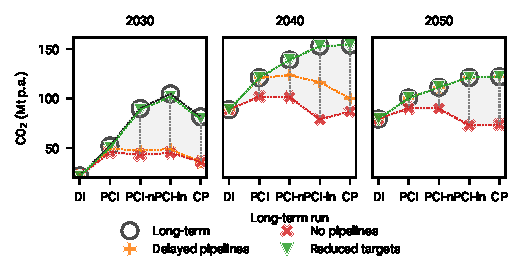
\includegraphics[width=\linewidth]{delta_balances_process emissions CC}
  \caption{$\Delta$\ce{CO2} balances --- Process emissions including Carbon Capture.}
  \label{fig:delta_balances_process_emissions_CC}
\end{figure}

\begin{figure}[htbp]
  \centering
  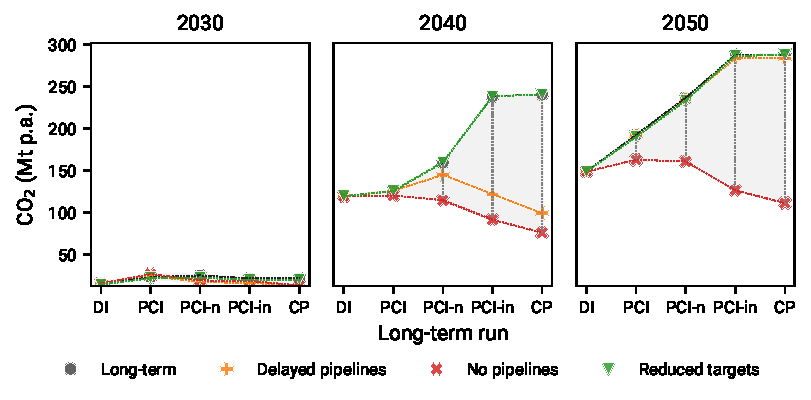
\includegraphics[width=\linewidth]{delta_balances_solid biomass for industry CC}
  \caption{$\Delta$\ce{CO2} balances --- Carbon capture from solid biomass for industry point sources.}
  \label{fig:delta_balances_biomass_industry_cc}
\end{figure}

\begin{figure}[htbp]
  \centering
  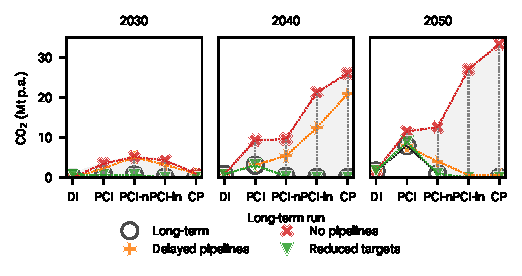
\includegraphics[width=\linewidth]{delta_balances_SMR CC}
  \caption{$\Delta$\ce{CO2} balances --- Carbon capture from SMR point sources.}
  \label{fig:delta_balances_smr_cc}
\end{figure}

\begin{figure}[htbp]
  \centering
  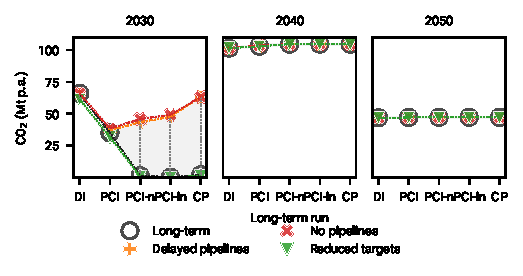
\includegraphics[width=\linewidth]{delta_balances_gas for industry CC}
  \caption{$\Delta$\ce{CO2} balances --- Carbon captured from gas for industry point sources.}
  \label{fig:delta_balances_gas_for_industry}
\end{figure}

\begin{figure}[htbp]
  \centering
  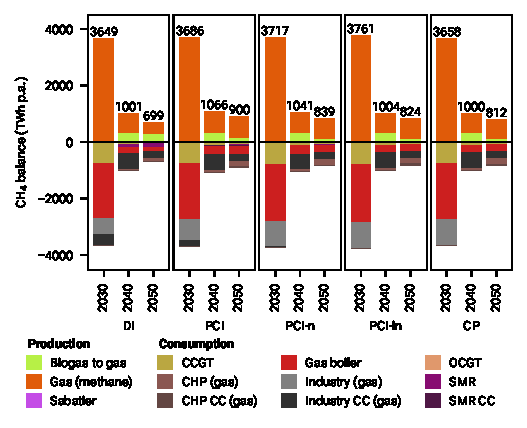
\includegraphics[width=\linewidth]{balances_overview_gas}
  \caption{\ce{CH4} balances in long-term scenarios.}
  \label{fig:balances_overview_gas}
\end{figure}

\begin{figure}[htbp]
  \centering
  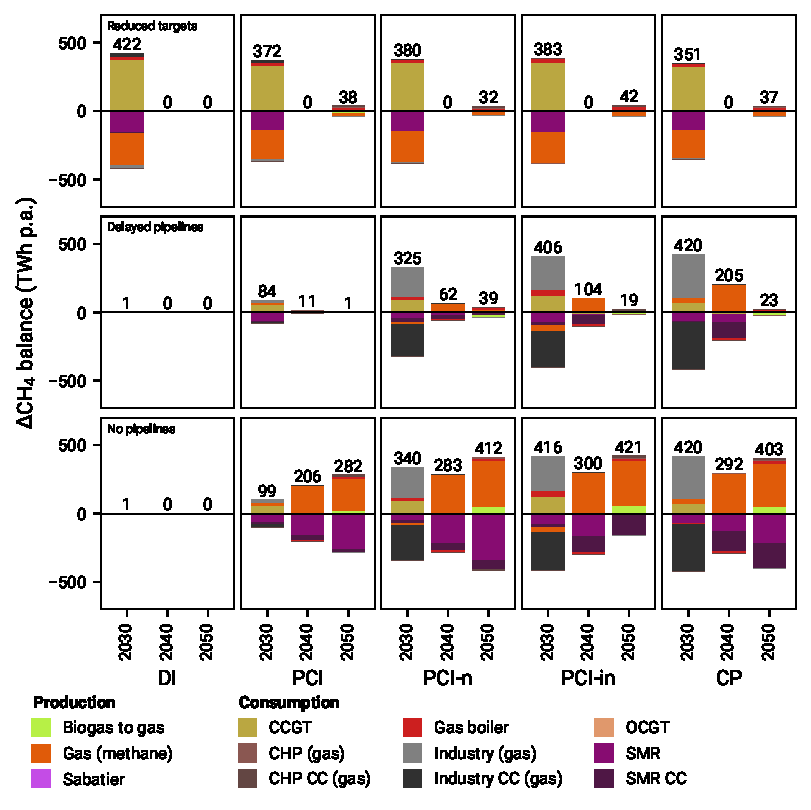
\includegraphics[width=\linewidth]{balances_overview_extended_gas}
  \caption{$\Delta$\ce{CH4} balances --- Short-term minus long-term runs.}
  \label{fig:balances_overview_extended_gas}
\end{figure}

\cleardoublepage


\begin{figure*}[htbp]
  \centering
  \begin{subfigure}[t]{0.33\textwidth}
      \vspace{0pt}
      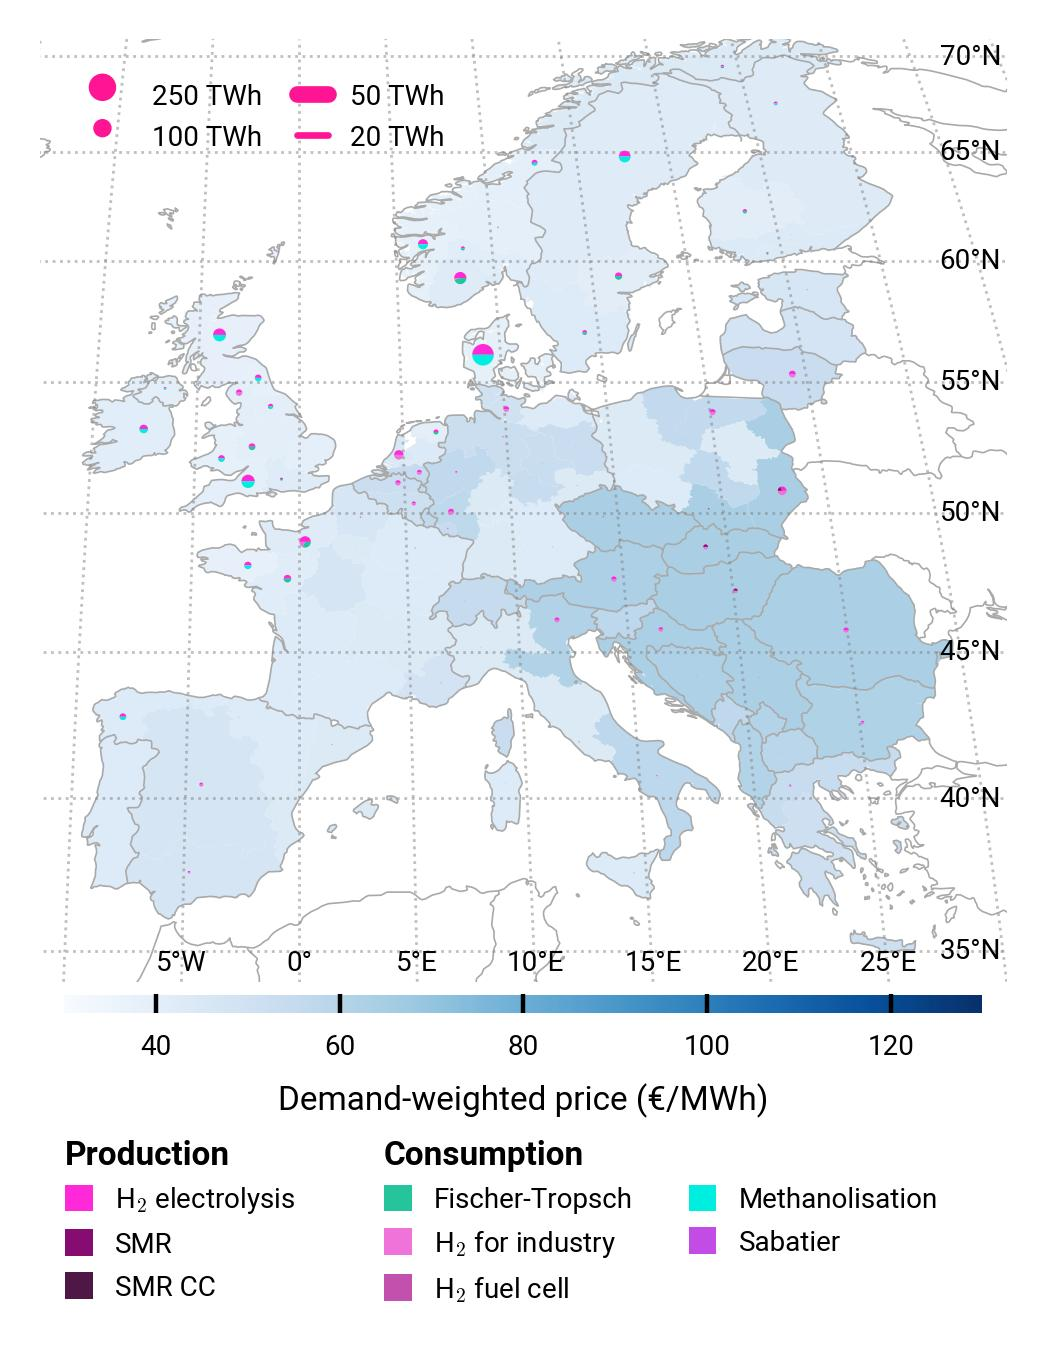
\includegraphics[width=1\textwidth]{maps/no-pipelines-no-pcipmi/base_s_adm___2030-balance_map_H2}
      \caption{\ce{H2} 2030.}
      \label{fig:DI_lt_2030_h2}
  \end{subfigure}
  \begin{subfigure}[t]{0.33\textwidth}
      \vspace{0pt}
      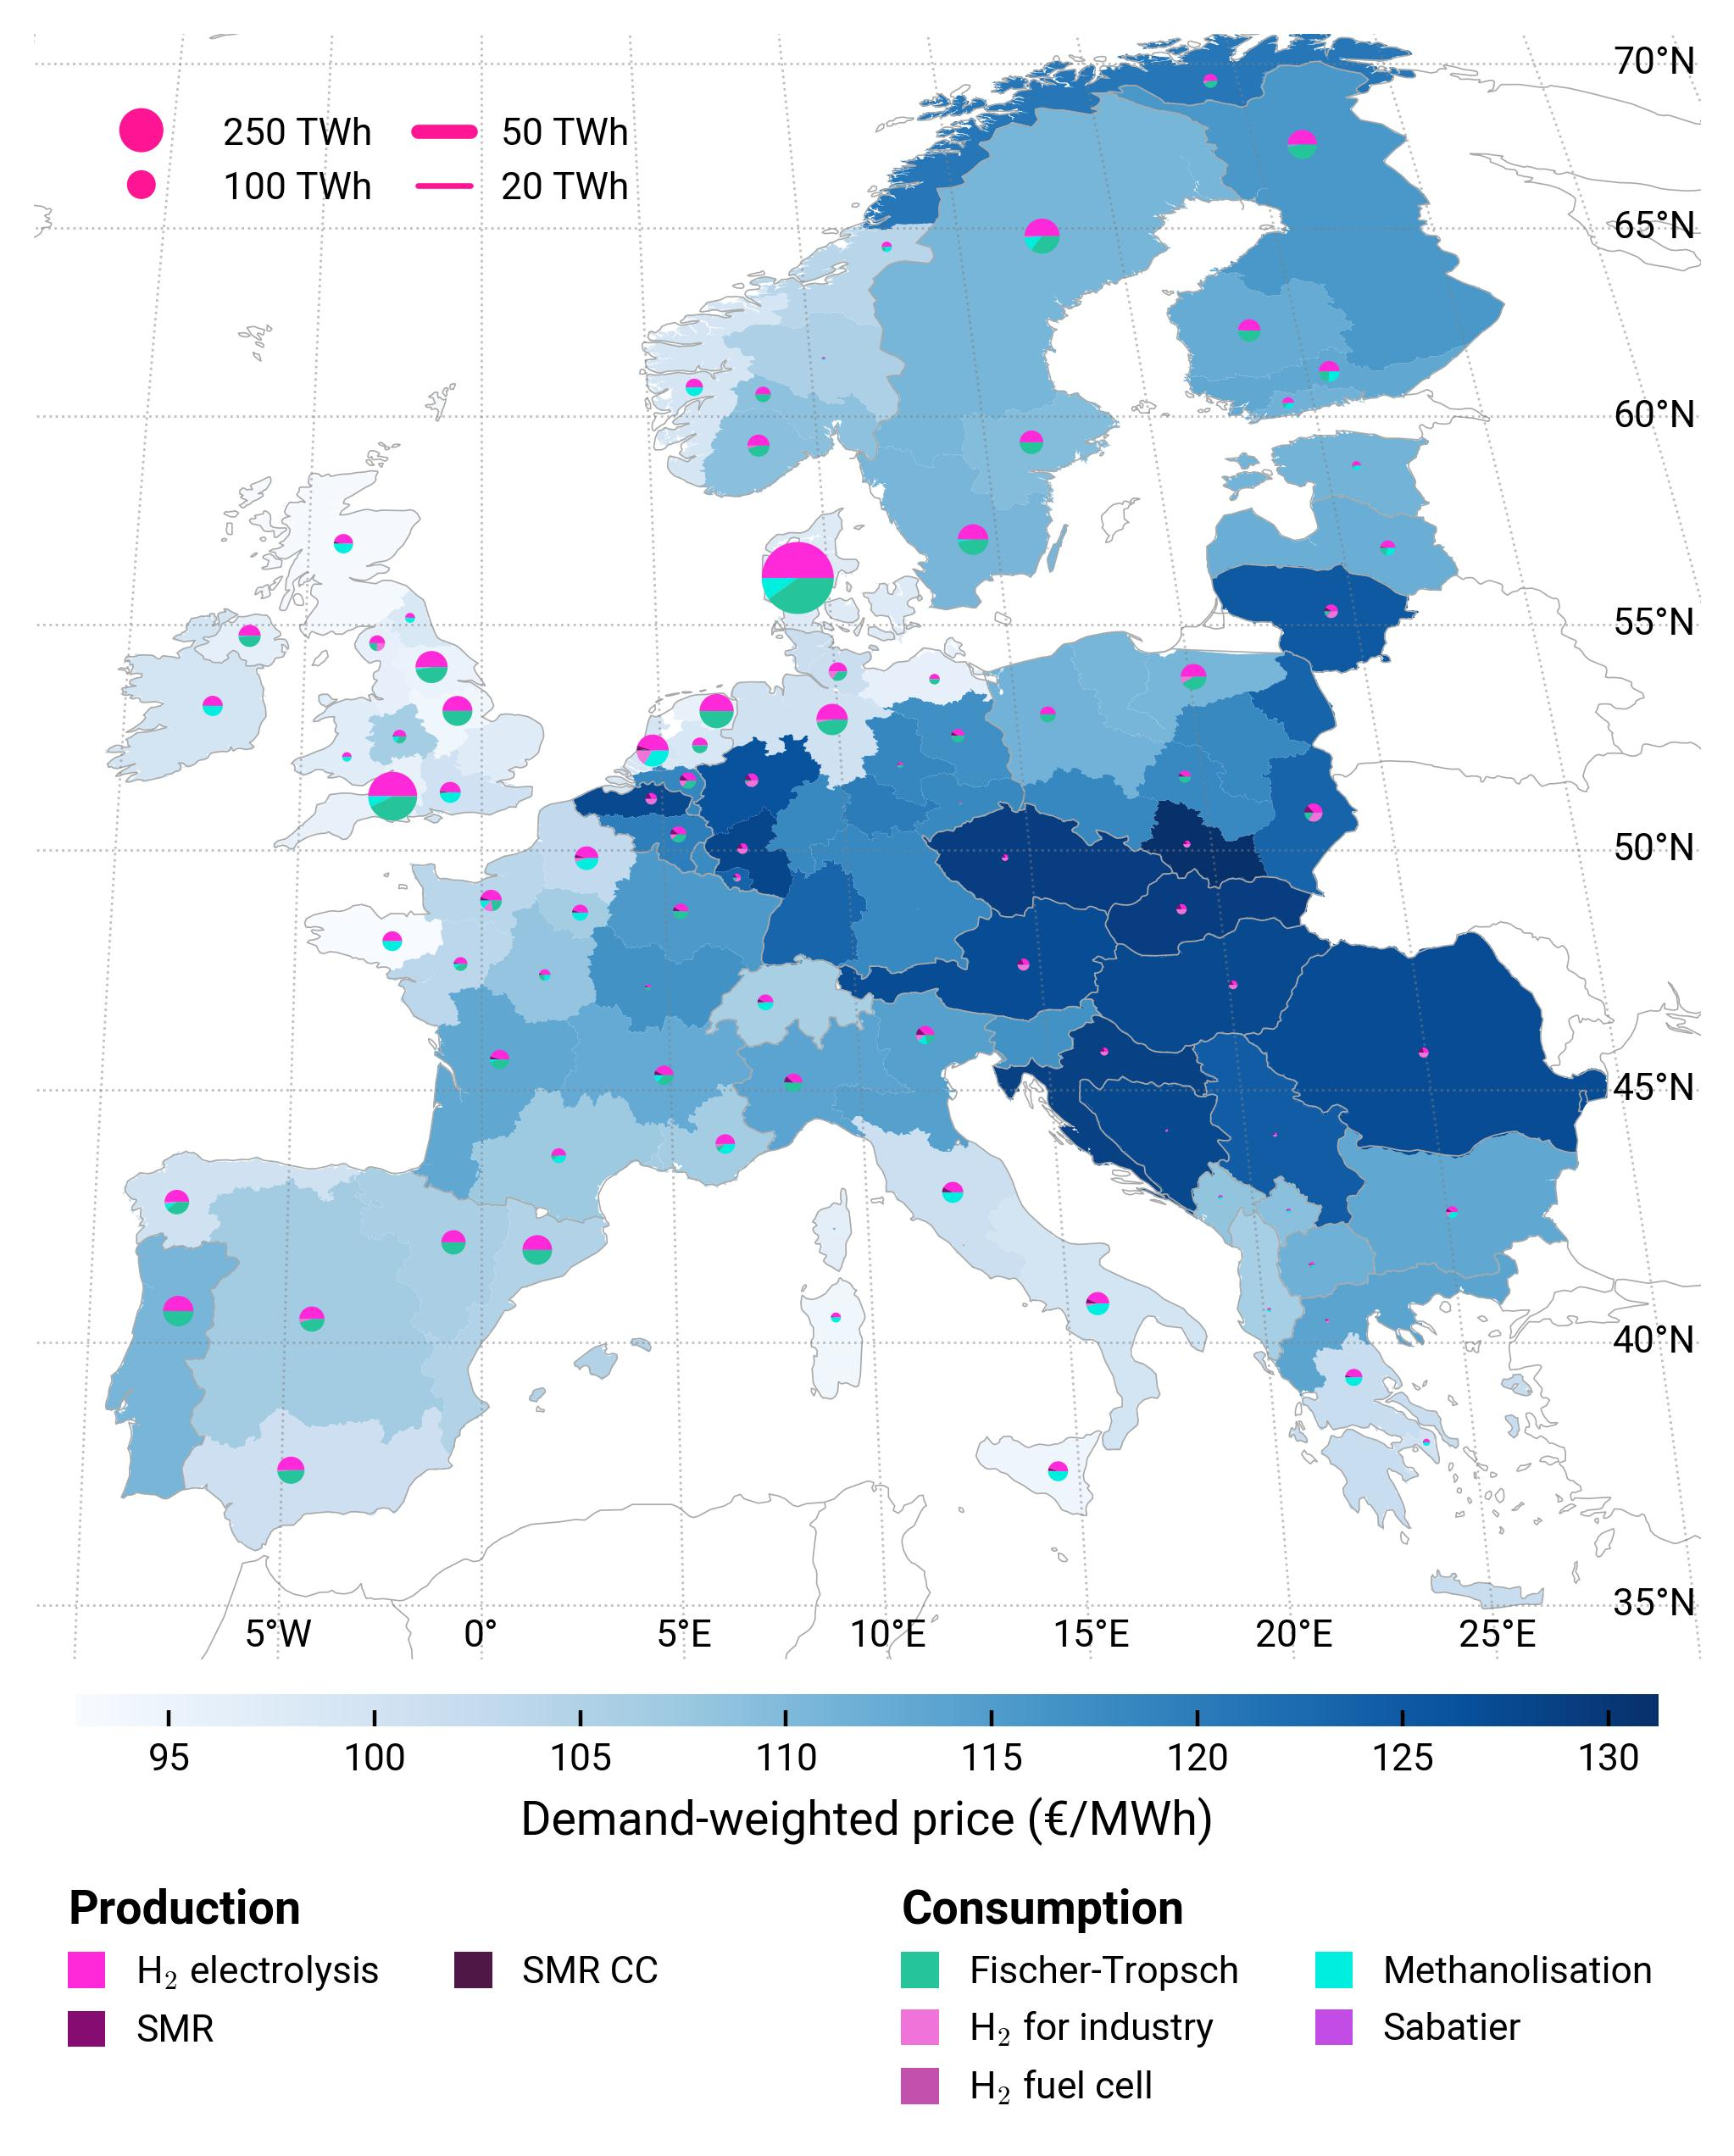
\includegraphics[width=1\textwidth]{maps/no-pipelines-no-pcipmi/base_s_adm___2040-balance_map_H2}
      \caption{\ce{H2} 2040.}
      \label{fig:DI_lt_2040_h2}
  \end{subfigure}
  \begin{subfigure}[t]{0.33\textwidth}
    \vspace{0pt}
    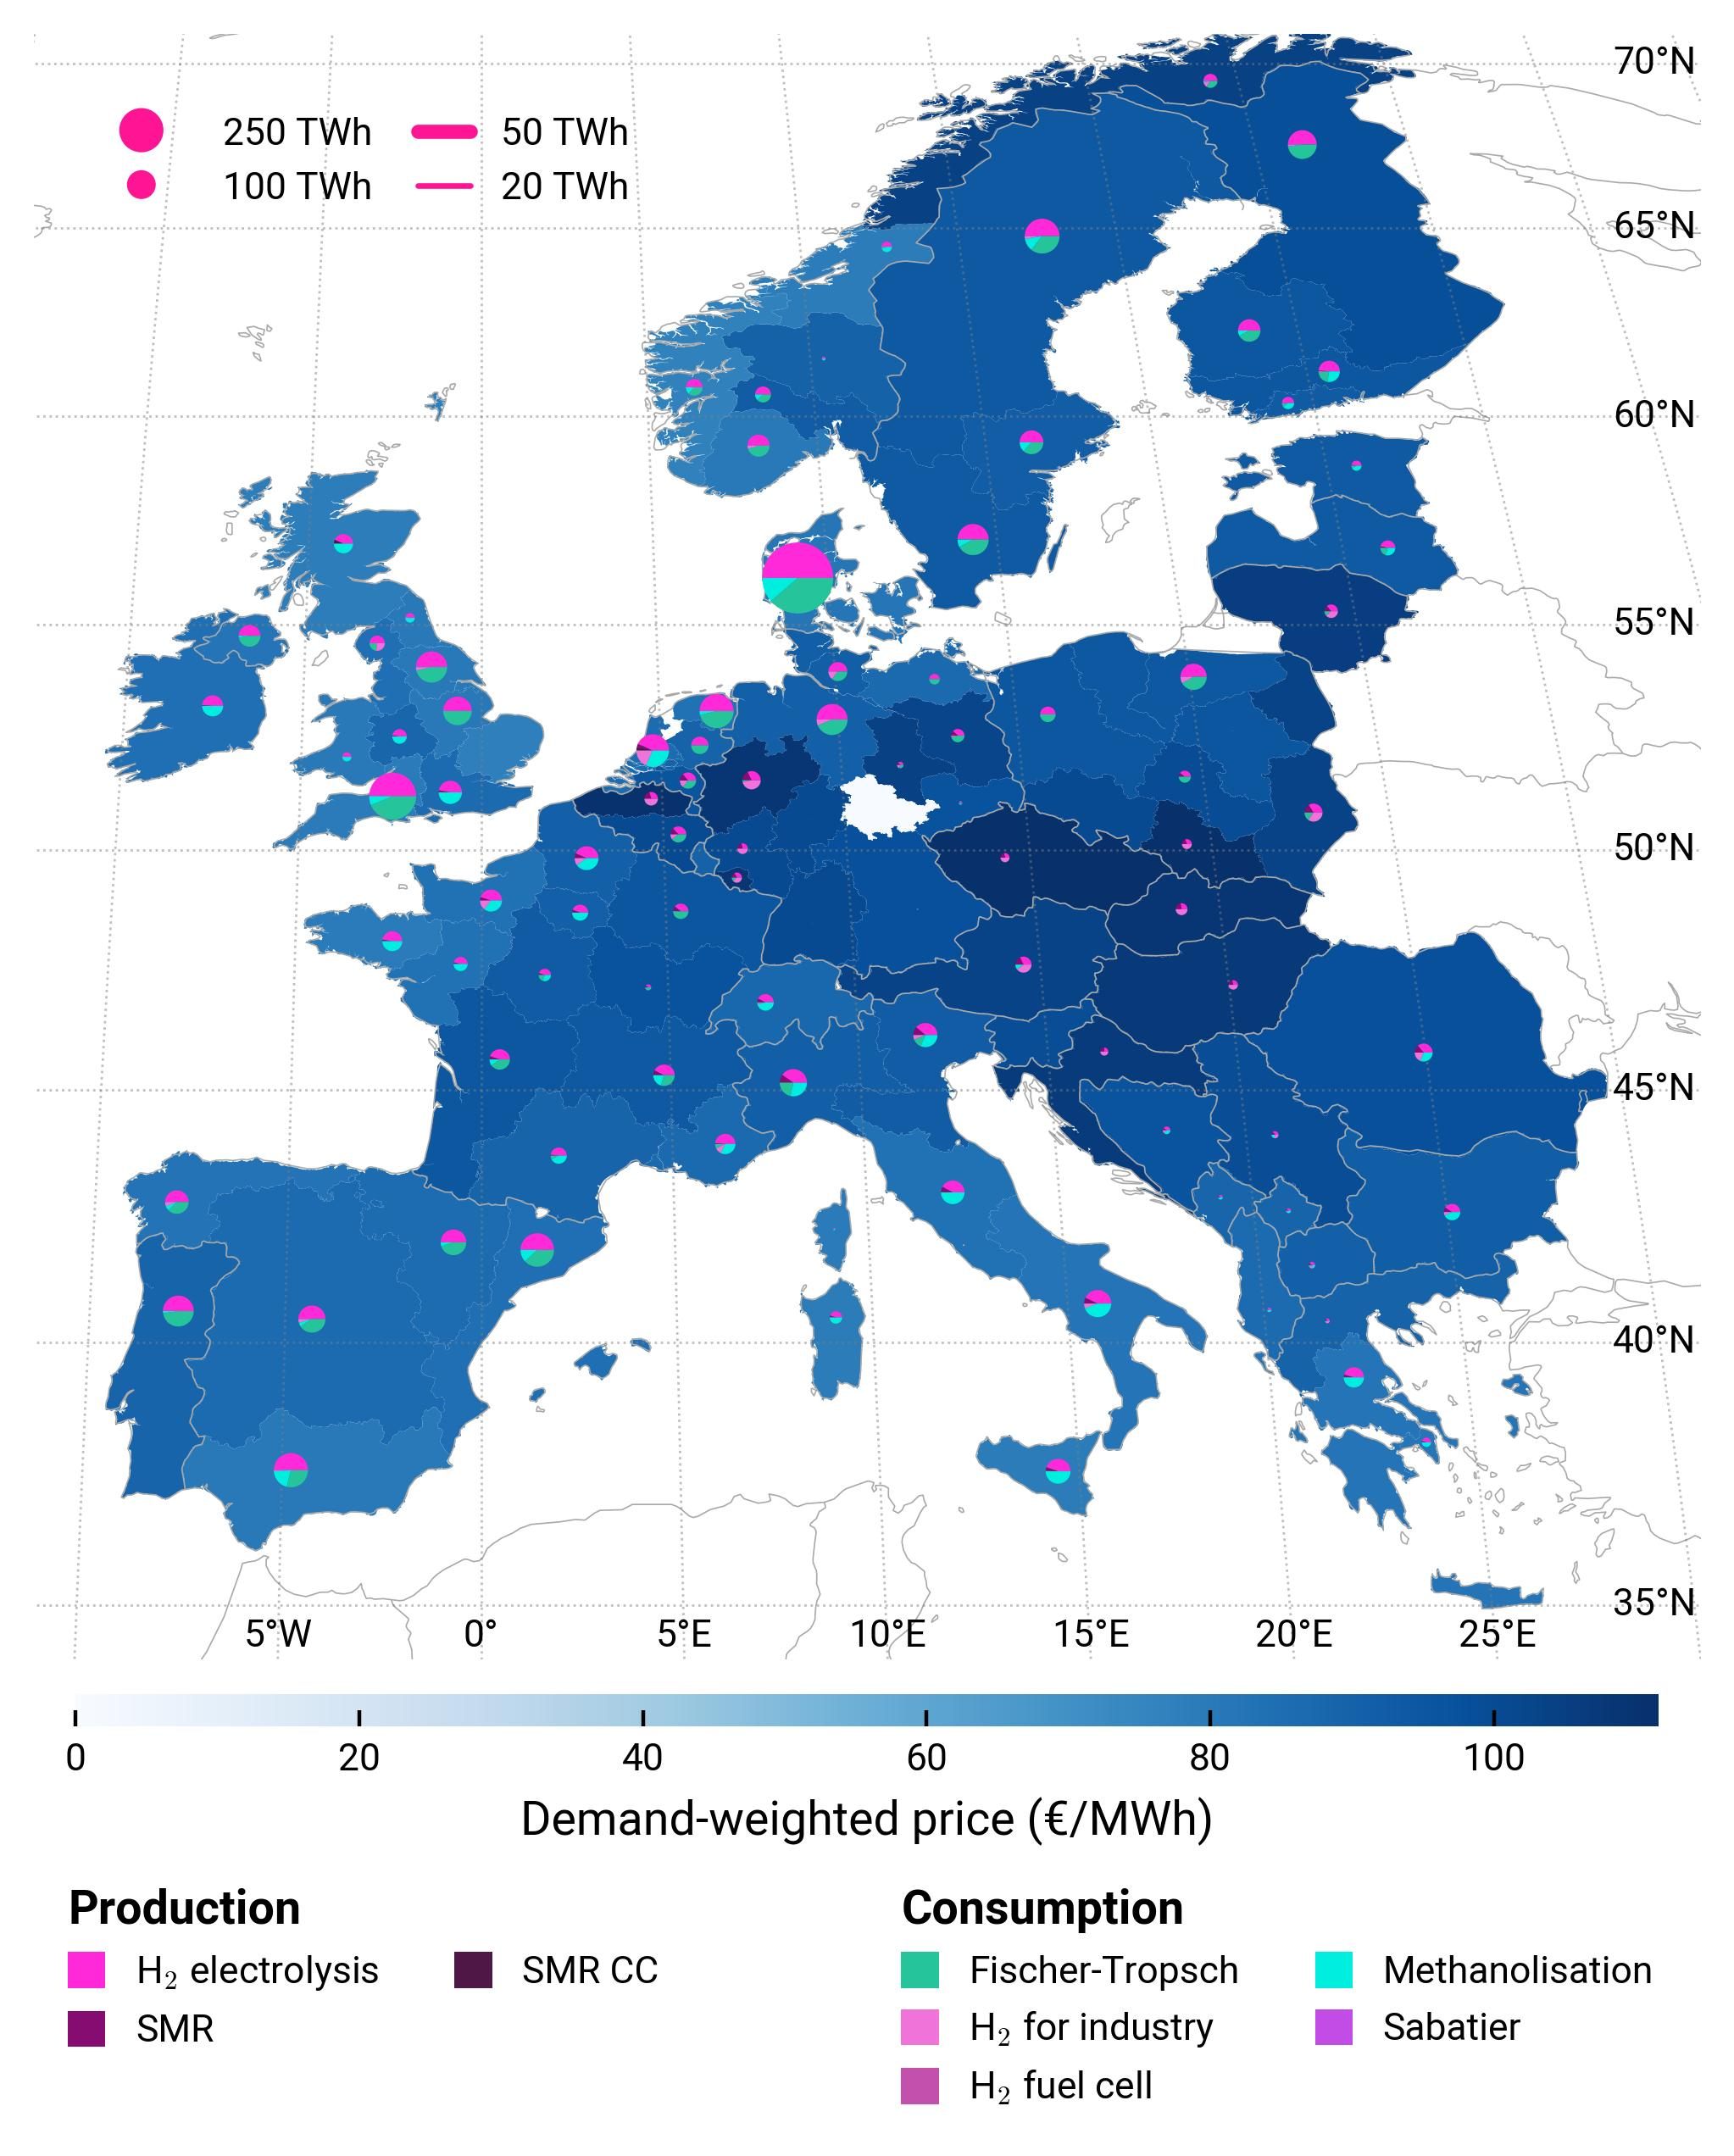
\includegraphics[width=1\textwidth]{maps/no-pipelines-no-pcipmi/base_s_adm___2050-balance_map_H2}
    \caption{\ce{H2} 2050.}
    \label{fig:DI_lt_2050_h2}
  \end{subfigure}
  \begin{subfigure}[t]{0.33\textwidth}
      \vspace{0pt}
      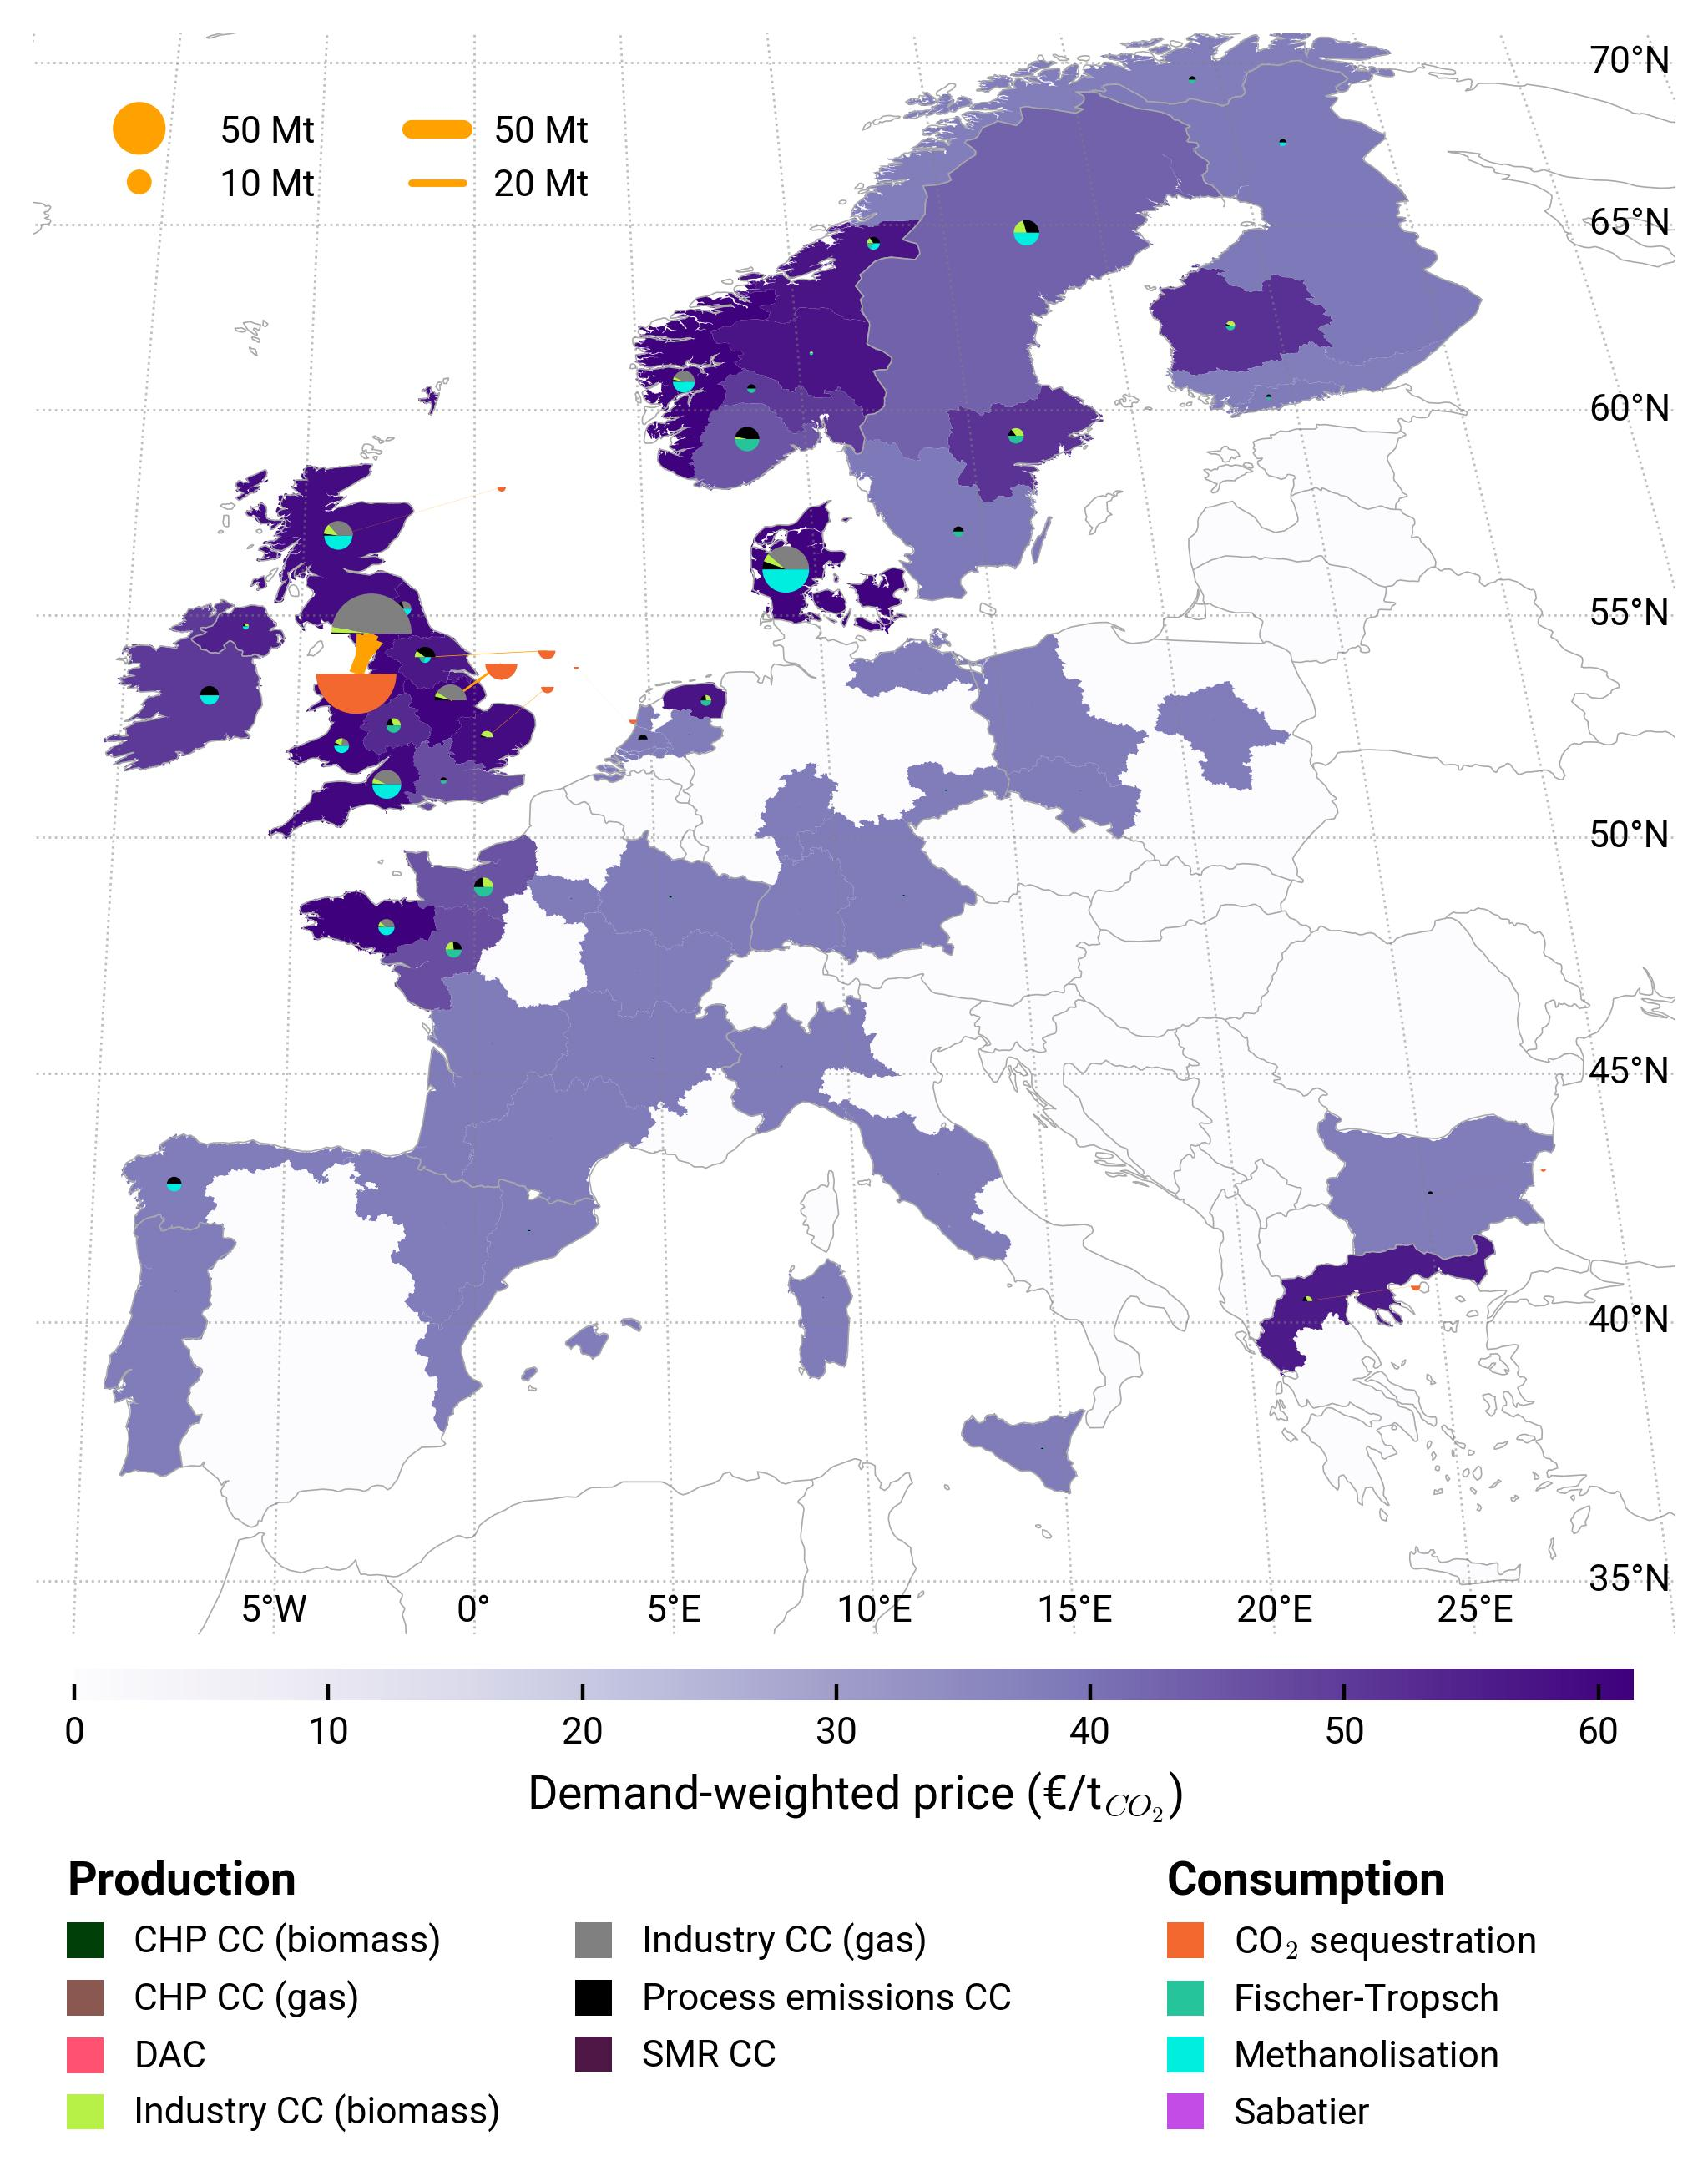
\includegraphics[width=1\textwidth]{maps/no-pipelines-no-pcipmi/base_s_adm___2030-balance_map_co2_stored} 
      \caption{\ce{CO2} 2030.}
      \label{fig:DI_lt_2030_co2}
  \end{subfigure}
  \begin{subfigure}[t]{0.33\textwidth}
      \vspace{0pt}
      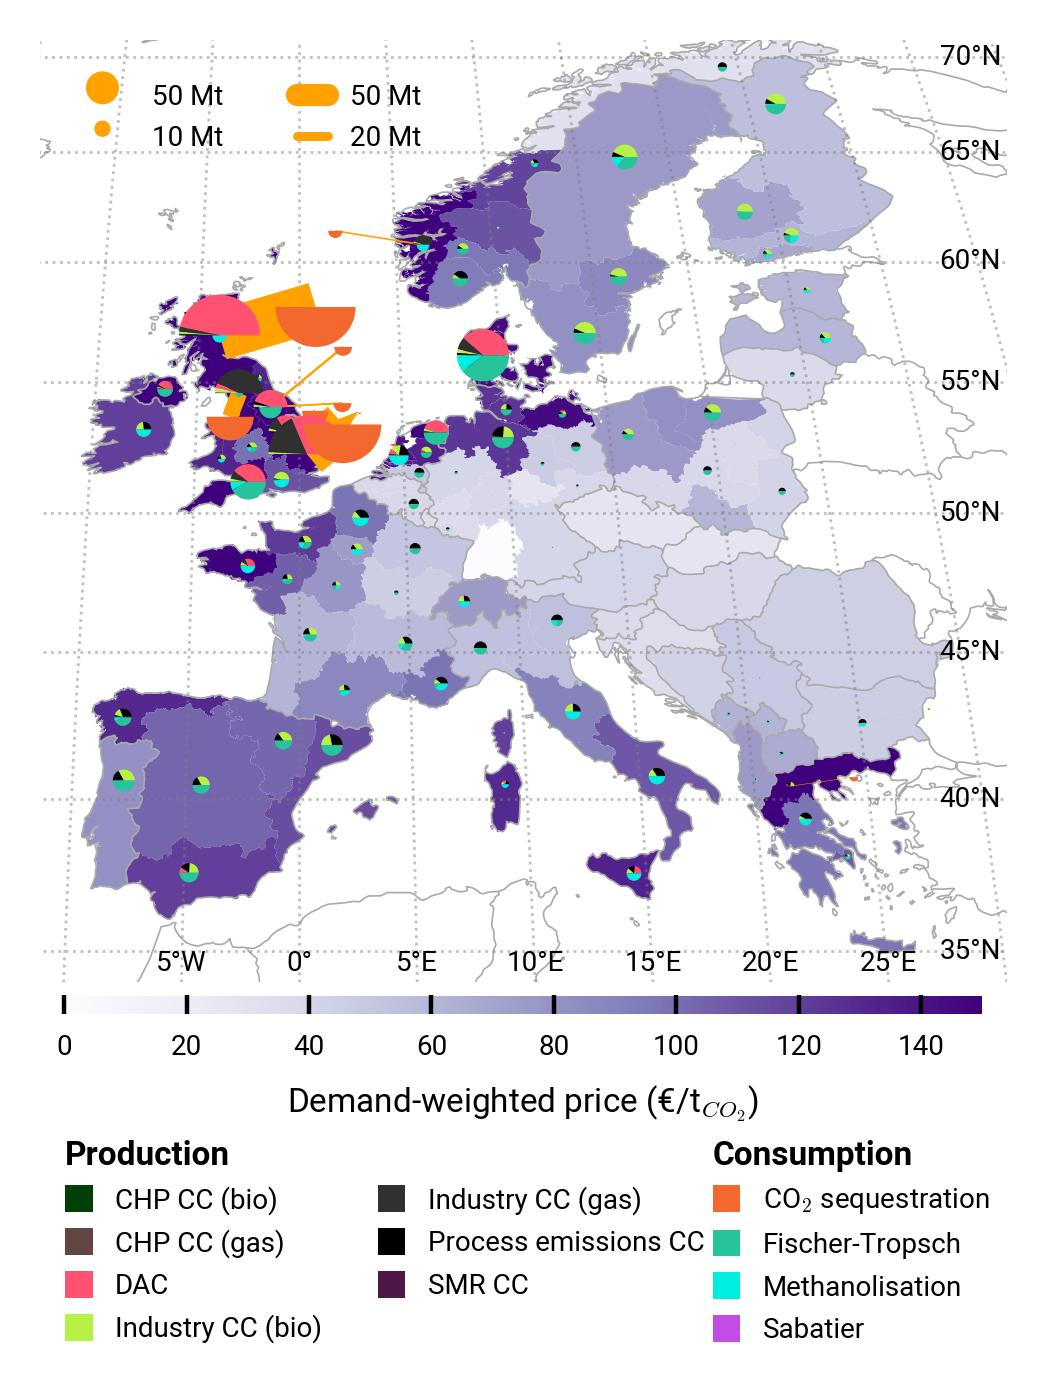
\includegraphics[width=1\textwidth]{maps/no-pipelines-no-pcipmi/base_s_adm___2040-balance_map_co2_stored} 
      \caption{\ce{CO2} 2040.}
      \label{fig:DI_lt_2040_co2}
  \end{subfigure}
  \begin{subfigure}[t]{0.33\textwidth}
      \vspace{0pt}
      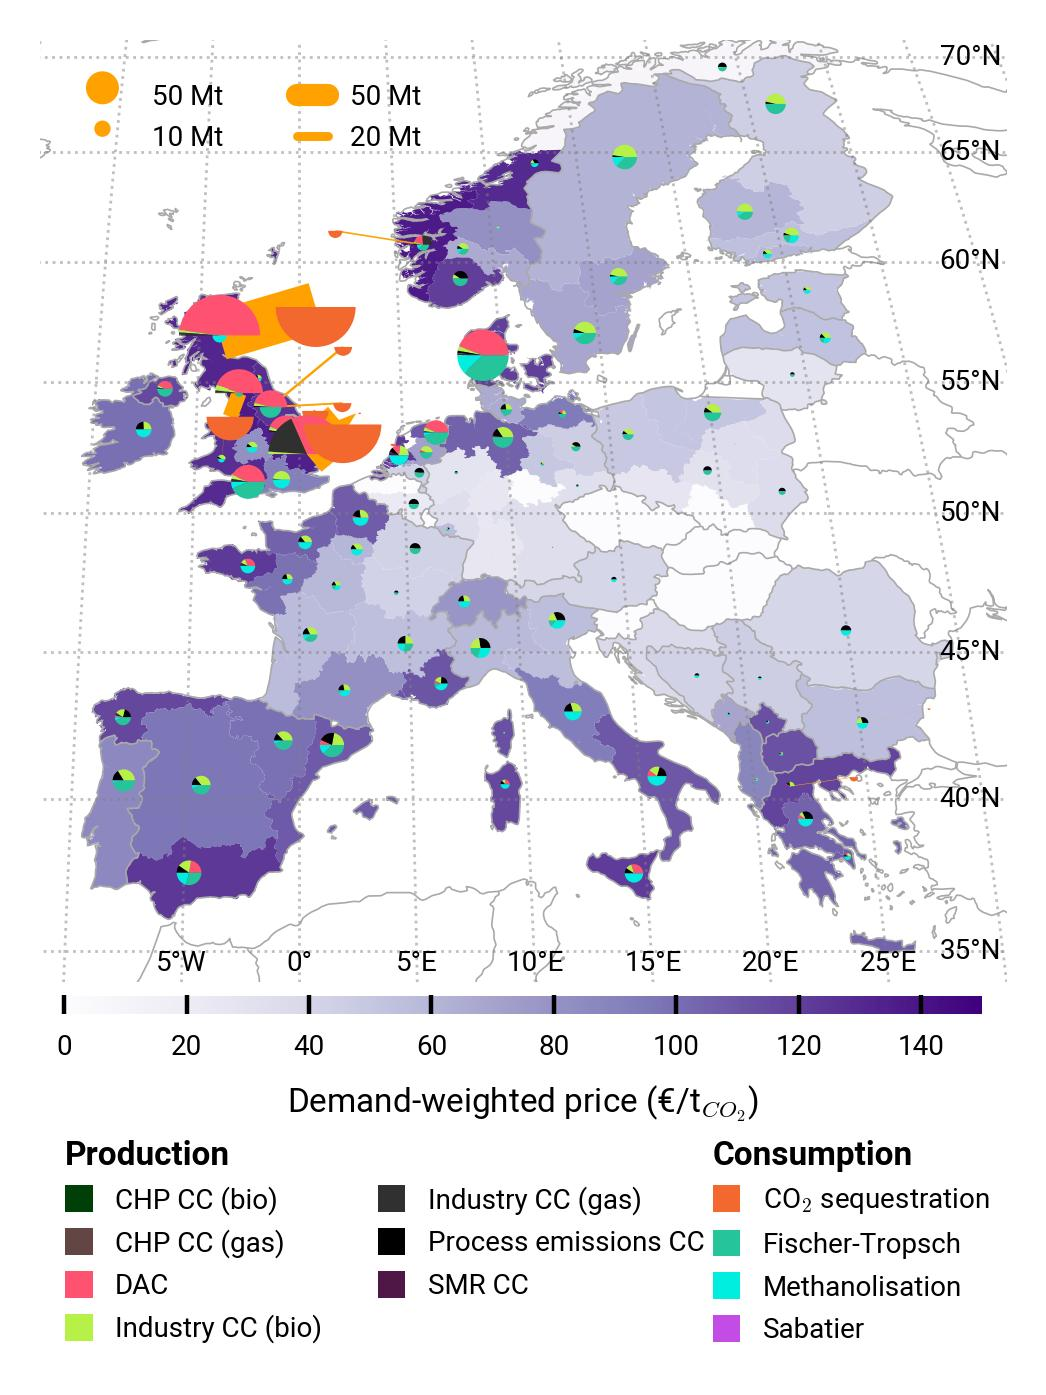
\includegraphics[width=1\textwidth]{maps/no-pipelines-no-pcipmi/base_s_adm___2050-balance_map_co2_stored} 
      \caption{\ce{CO2} 2050.}
      \label{fig:DI_lt_2050_co2}
  \end{subfigure}
  \vspace{0.3cm}
  \caption{\textit{Decentral Islands} long-term scenario --- Regional distribution of \ce{H2} and \ce{CO2} production, utilisation, storage, transport and price. \textit{Note that both the \ce{H2} and \ce{CO2} price refer to their value as a commodity, i.e., price is higher where there is a demand for it.}}
  \label{fig:DI_lt}
\end{figure*}


\begin{figure*}[htbp]
  \centering
  \begin{subfigure}[t]{0.33\textwidth}
      \vspace{0pt}
      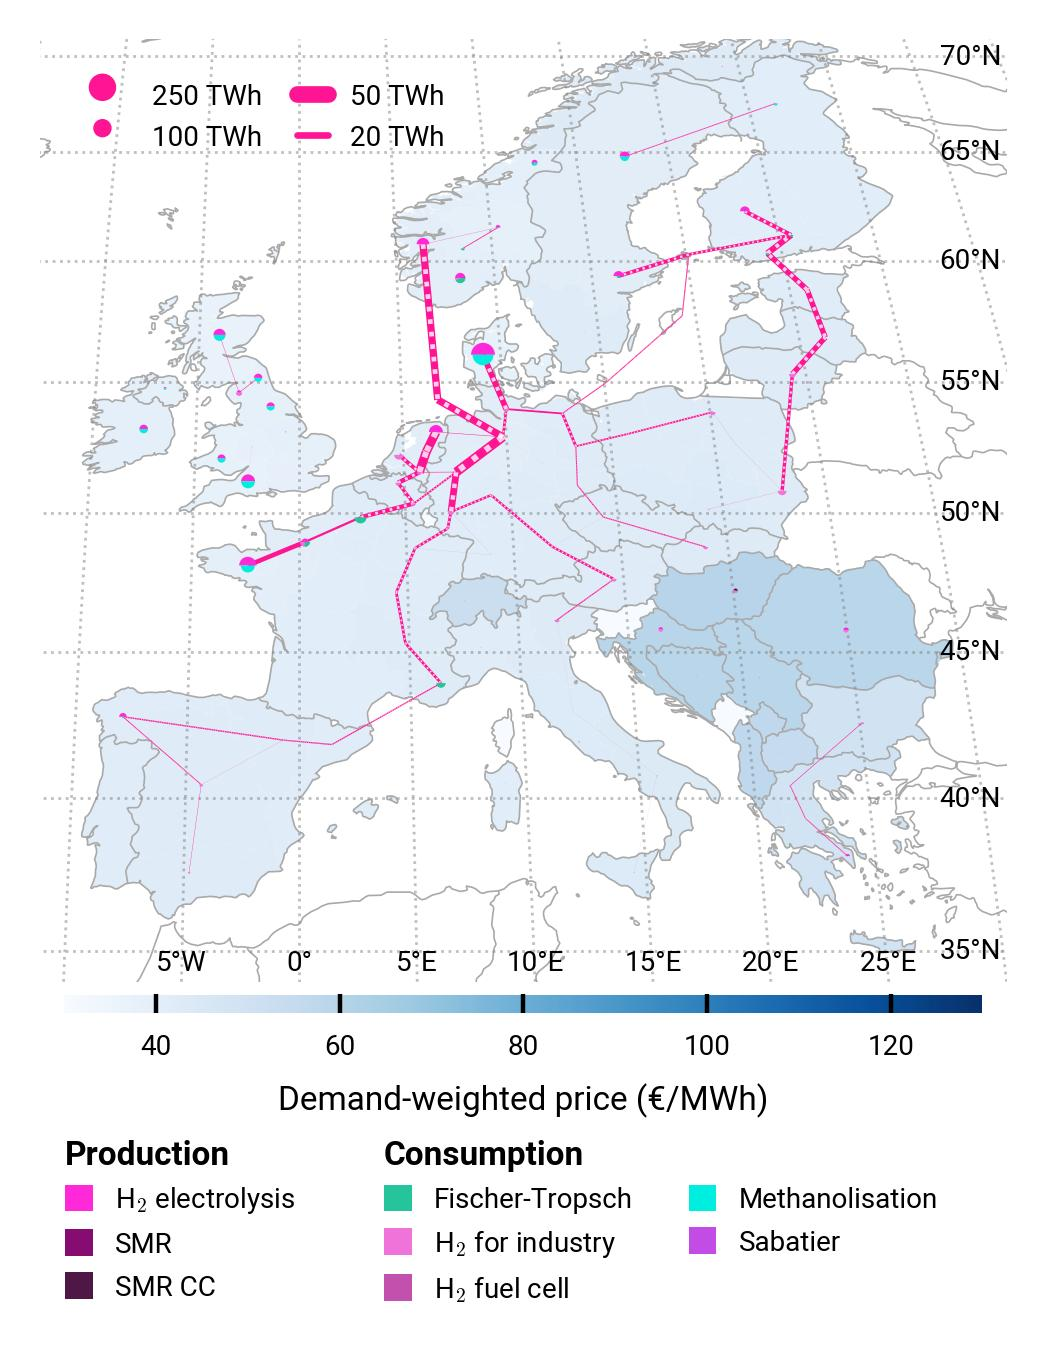
\includegraphics[width=1\textwidth]{maps/pcipmi-national-expansion/base_s_adm___2030-balance_map_H2}
      \caption{\ce{H2} 2030.}
      \label{fig:PCI-n_lt_2030_h2}
  \end{subfigure}
  \begin{subfigure}[t]{0.33\textwidth}
      \vspace{0pt}
      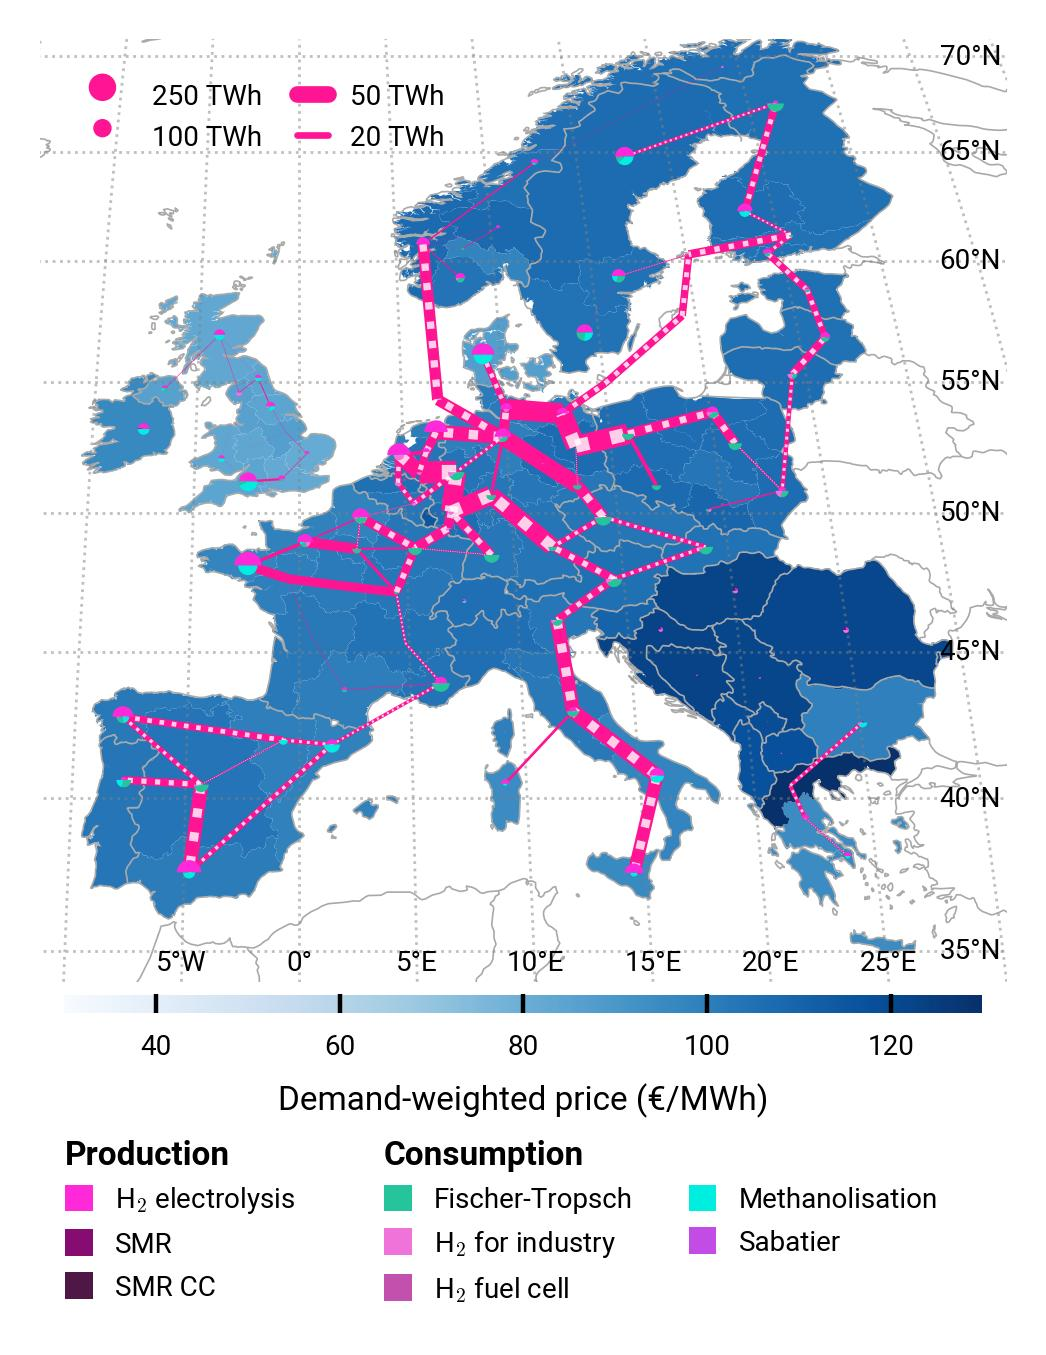
\includegraphics[width=1\textwidth]{maps/pcipmi-national-expansion/base_s_adm___2040-balance_map_H2}
      \caption{\ce{H2} 2040.}
      \label{fig:PCI-n_lt_2040_h2}
  \end{subfigure}
  \begin{subfigure}[t]{0.33\textwidth}
    \vspace{0pt}
    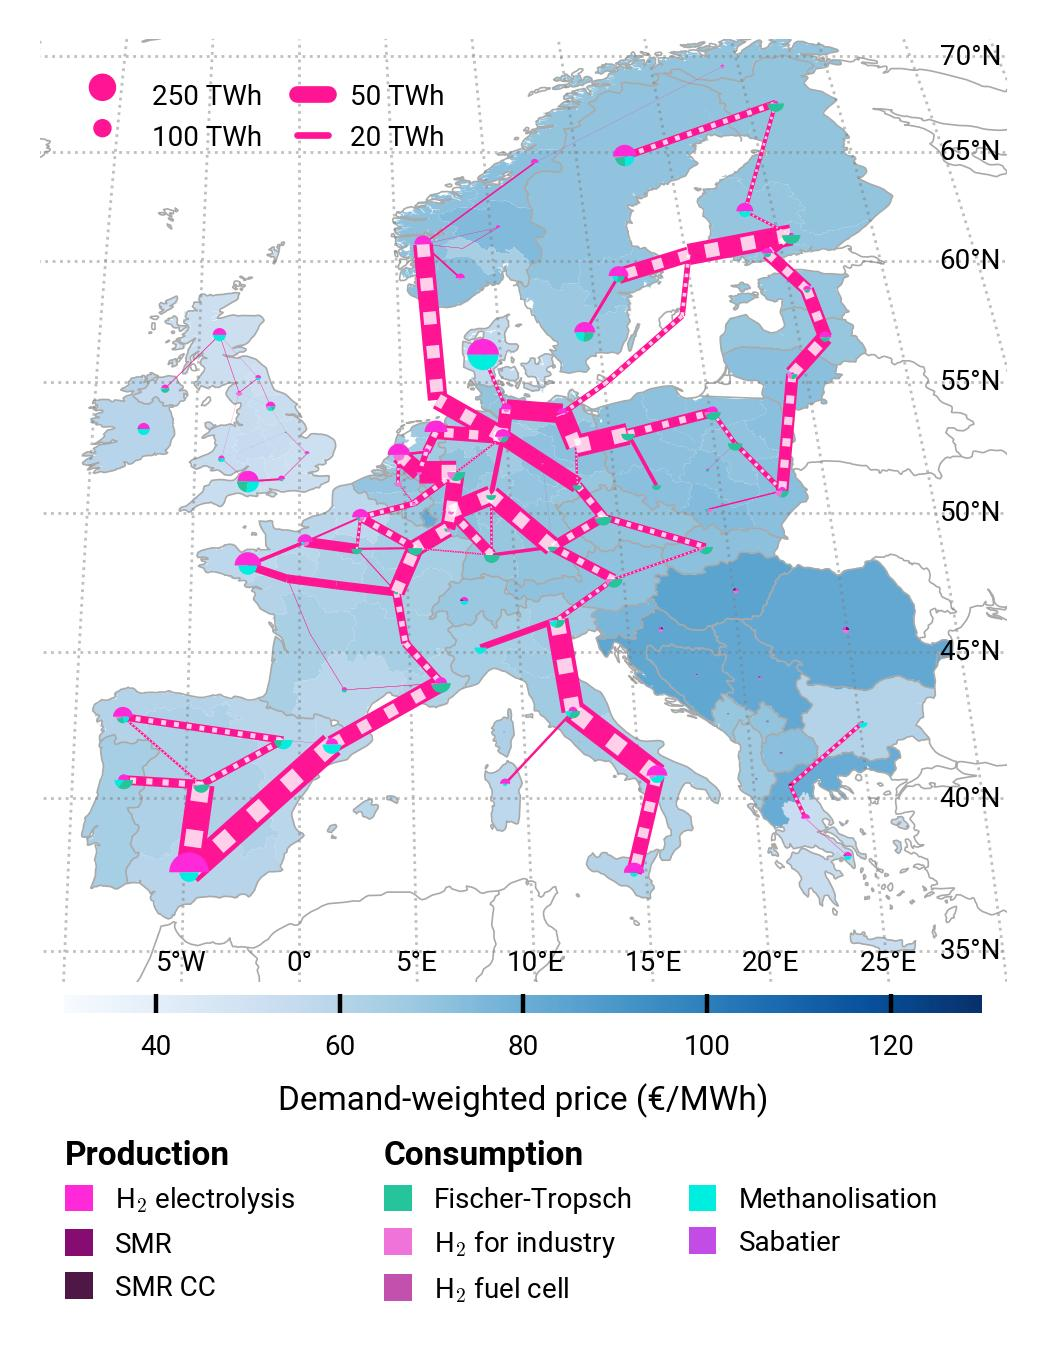
\includegraphics[width=1\textwidth]{maps/pcipmi-national-expansion/base_s_adm___2050-balance_map_H2}
    \caption{\ce{H2} 2050.}
    \label{fig:PCI-n_lt_2050_h2}
  \end{subfigure}
  \begin{subfigure}[t]{0.33\textwidth}
      \vspace{0pt}
      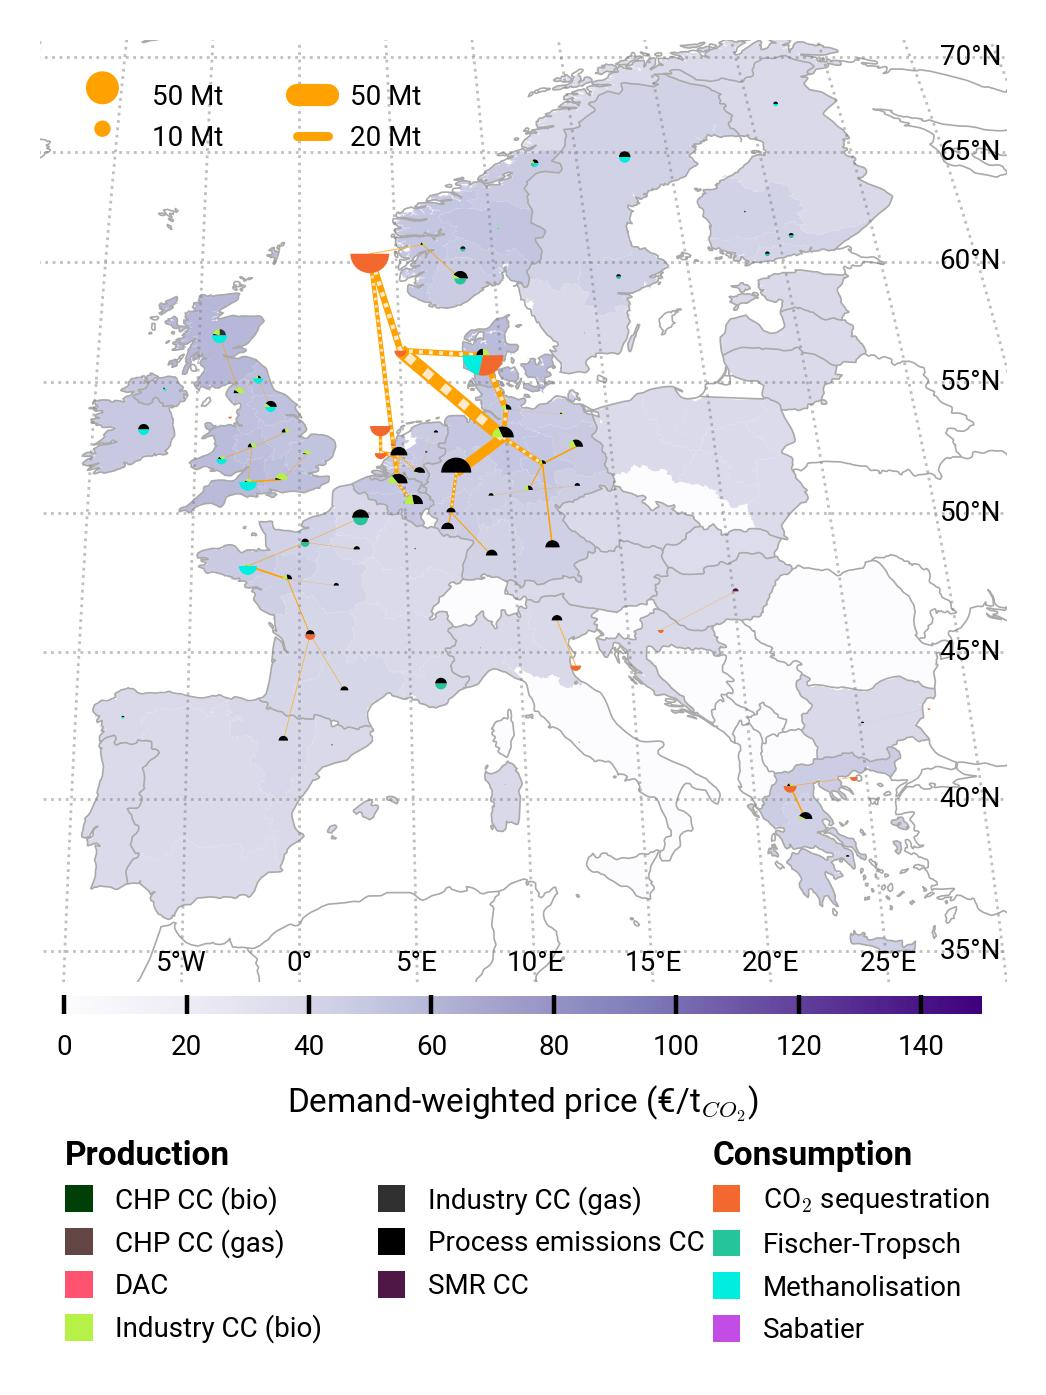
\includegraphics[width=1\textwidth]{maps/pcipmi-national-expansion/base_s_adm___2030-balance_map_co2_stored} 
      \caption{\ce{CO2} 2030.}
      \label{fig:PCI-n_lt_2030_co2}
  \end{subfigure}
  \begin{subfigure}[t]{0.33\textwidth}
      \vspace{0pt}
      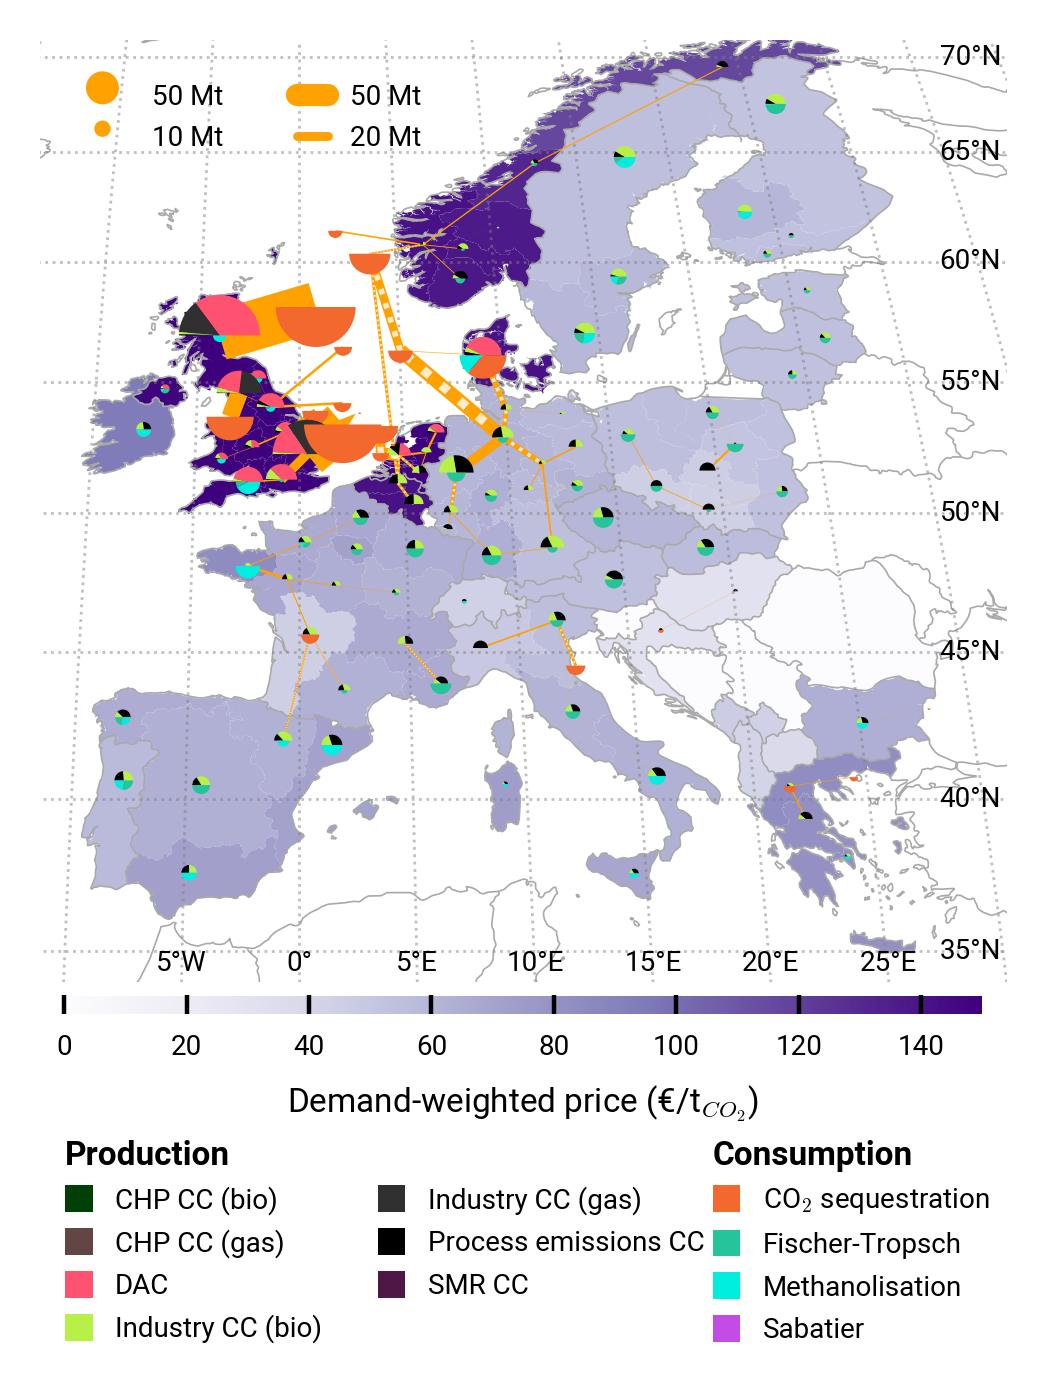
\includegraphics[width=1\textwidth]{maps/pcipmi-national-expansion/base_s_adm___2040-balance_map_co2_stored} 
      \caption{\ce{CO2} 2040.}
      \label{fig:PCI-n_lt_2040_co2}
  \end{subfigure}
  \begin{subfigure}[t]{0.33\textwidth}
      \vspace{0pt}
      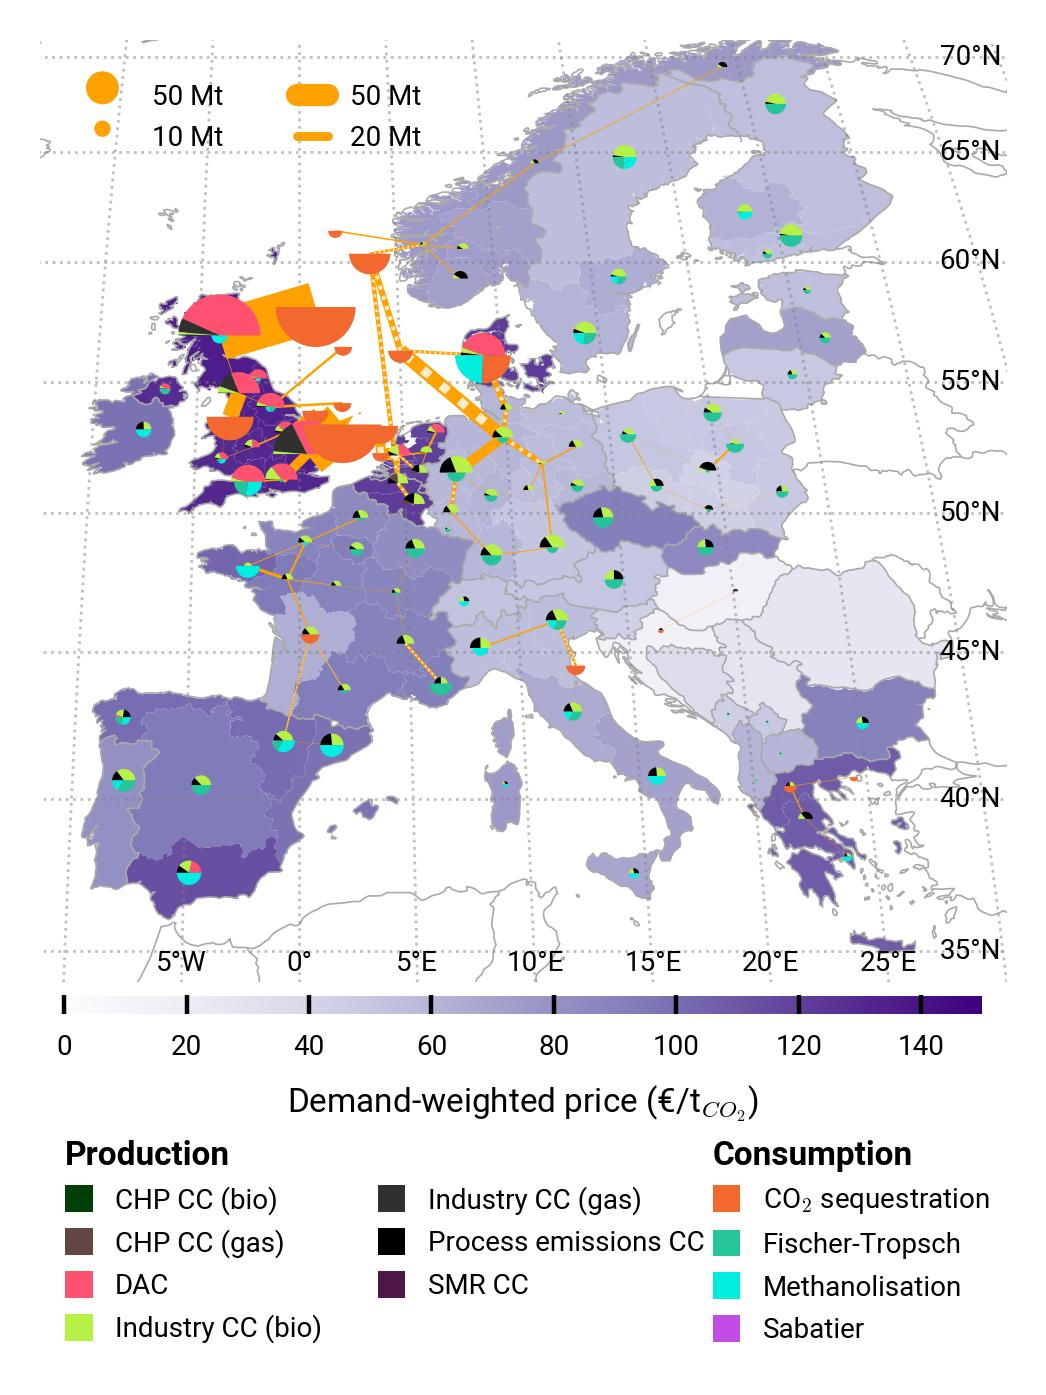
\includegraphics[width=1\textwidth]{maps/pcipmi-national-expansion/base_s_adm___2050-balance_map_co2_stored} 
      \caption{\ce{CO2} 2050.}
      \label{fig:PCI-n_lt_2050_co2}
  \end{subfigure}
  \vspace{0.3cm}
  \caption{\textit{PCI-PMI nat.} long-term scenario --- Regional distribution of \ce{H2} and \ce{CO2} production, utilisation, storage, transport and price. \textit{Note that both the \ce{H2} and \ce{CO2} price refer to their value as a commodity, i.e., price is higher where there is a demand for it.}}
  \label{fig:PCI-n_lt}
\end{figure*}

\begin{figure*}[htbp]
  \centering
  \begin{subfigure}[t]{0.33\textwidth}
      \vspace{0pt}
      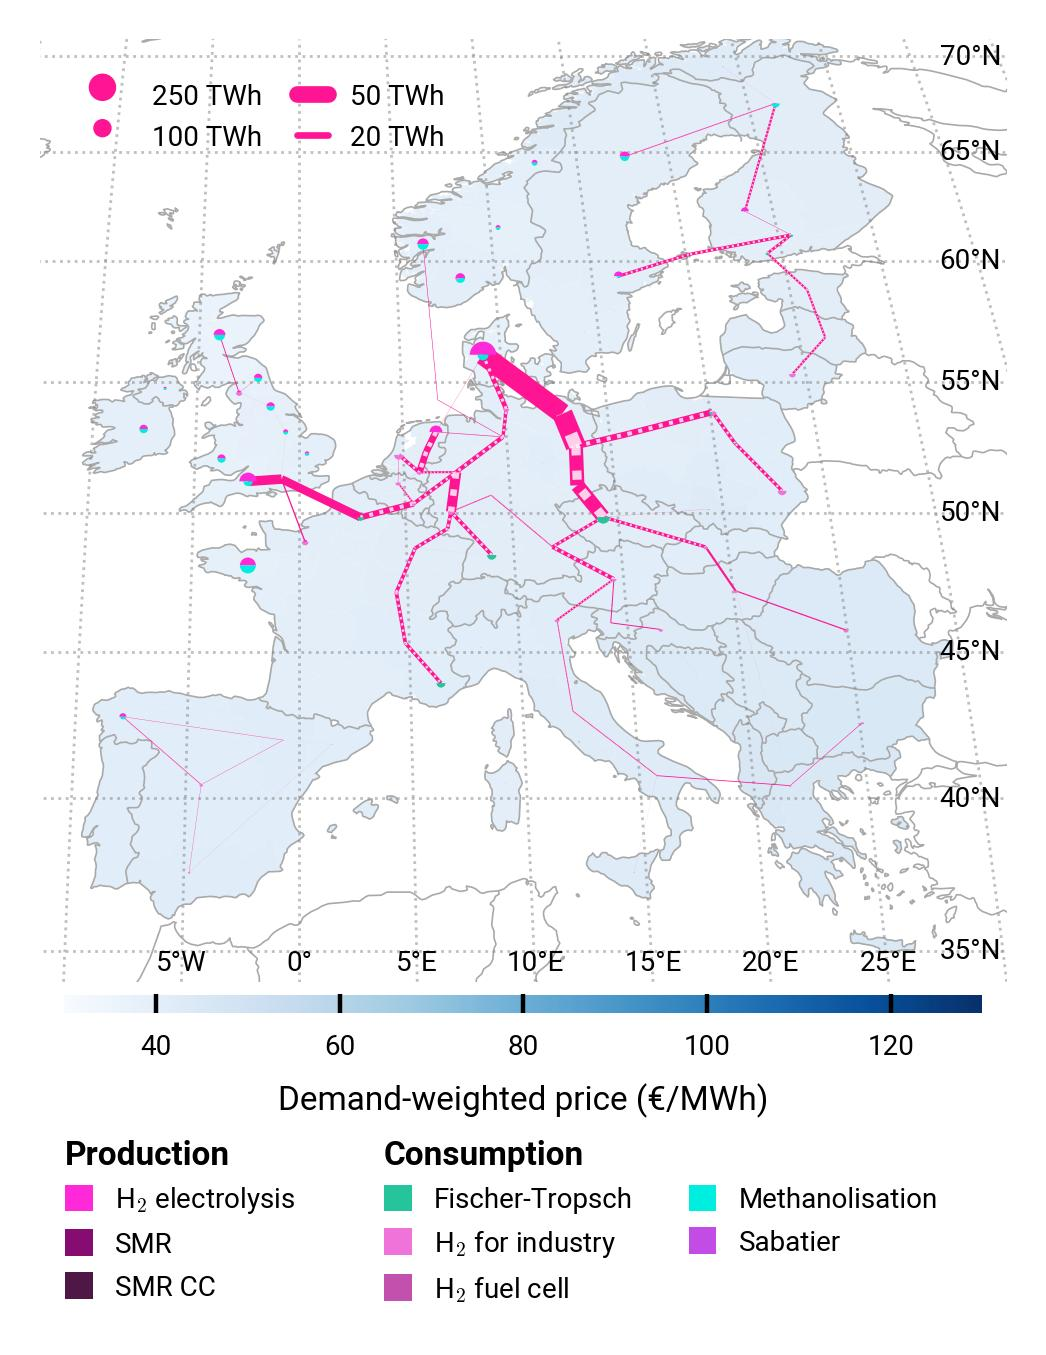
\includegraphics[width=1\textwidth]{maps/pcipmi-national-international-expansion/base_s_adm___2030-balance_map_H2}
      \caption{\ce{H2} 2030.}
      \label{fig:PCI-in_lt_2030_h2}
  \end{subfigure}
  \begin{subfigure}[t]{0.33\textwidth}
      \vspace{0pt}
      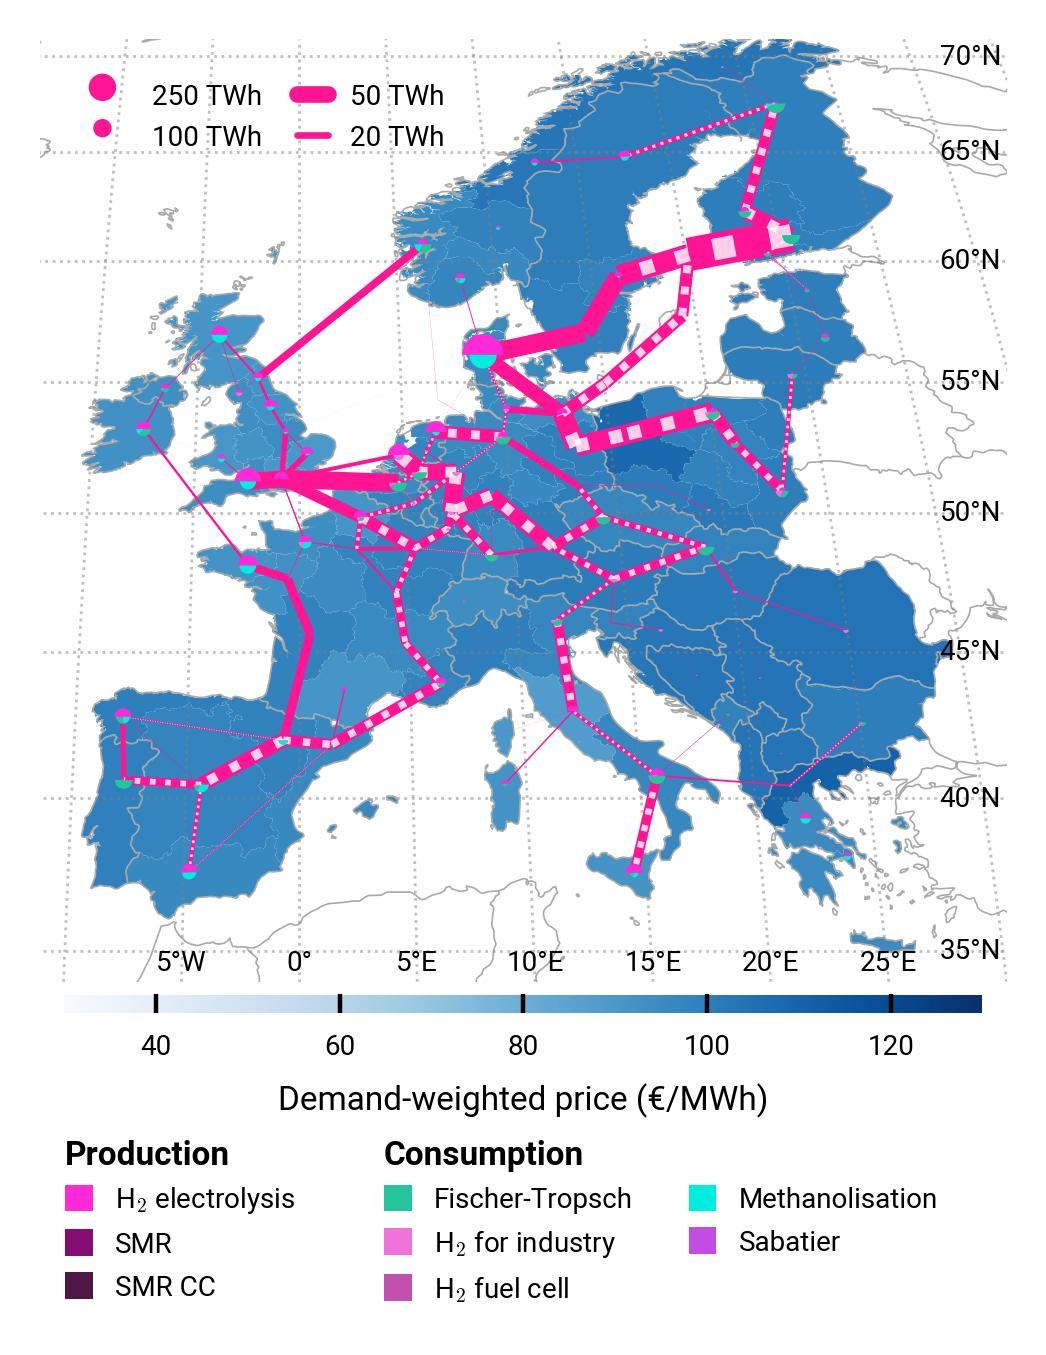
\includegraphics[width=1\textwidth]{maps/pcipmi-national-international-expansion/base_s_adm___2040-balance_map_H2}
      \caption{\ce{H2} 2040.}
      \label{fig:PCI-in_lt_2040_h2}
  \end{subfigure}
  \begin{subfigure}[t]{0.33\textwidth}
    \vspace{0pt}
    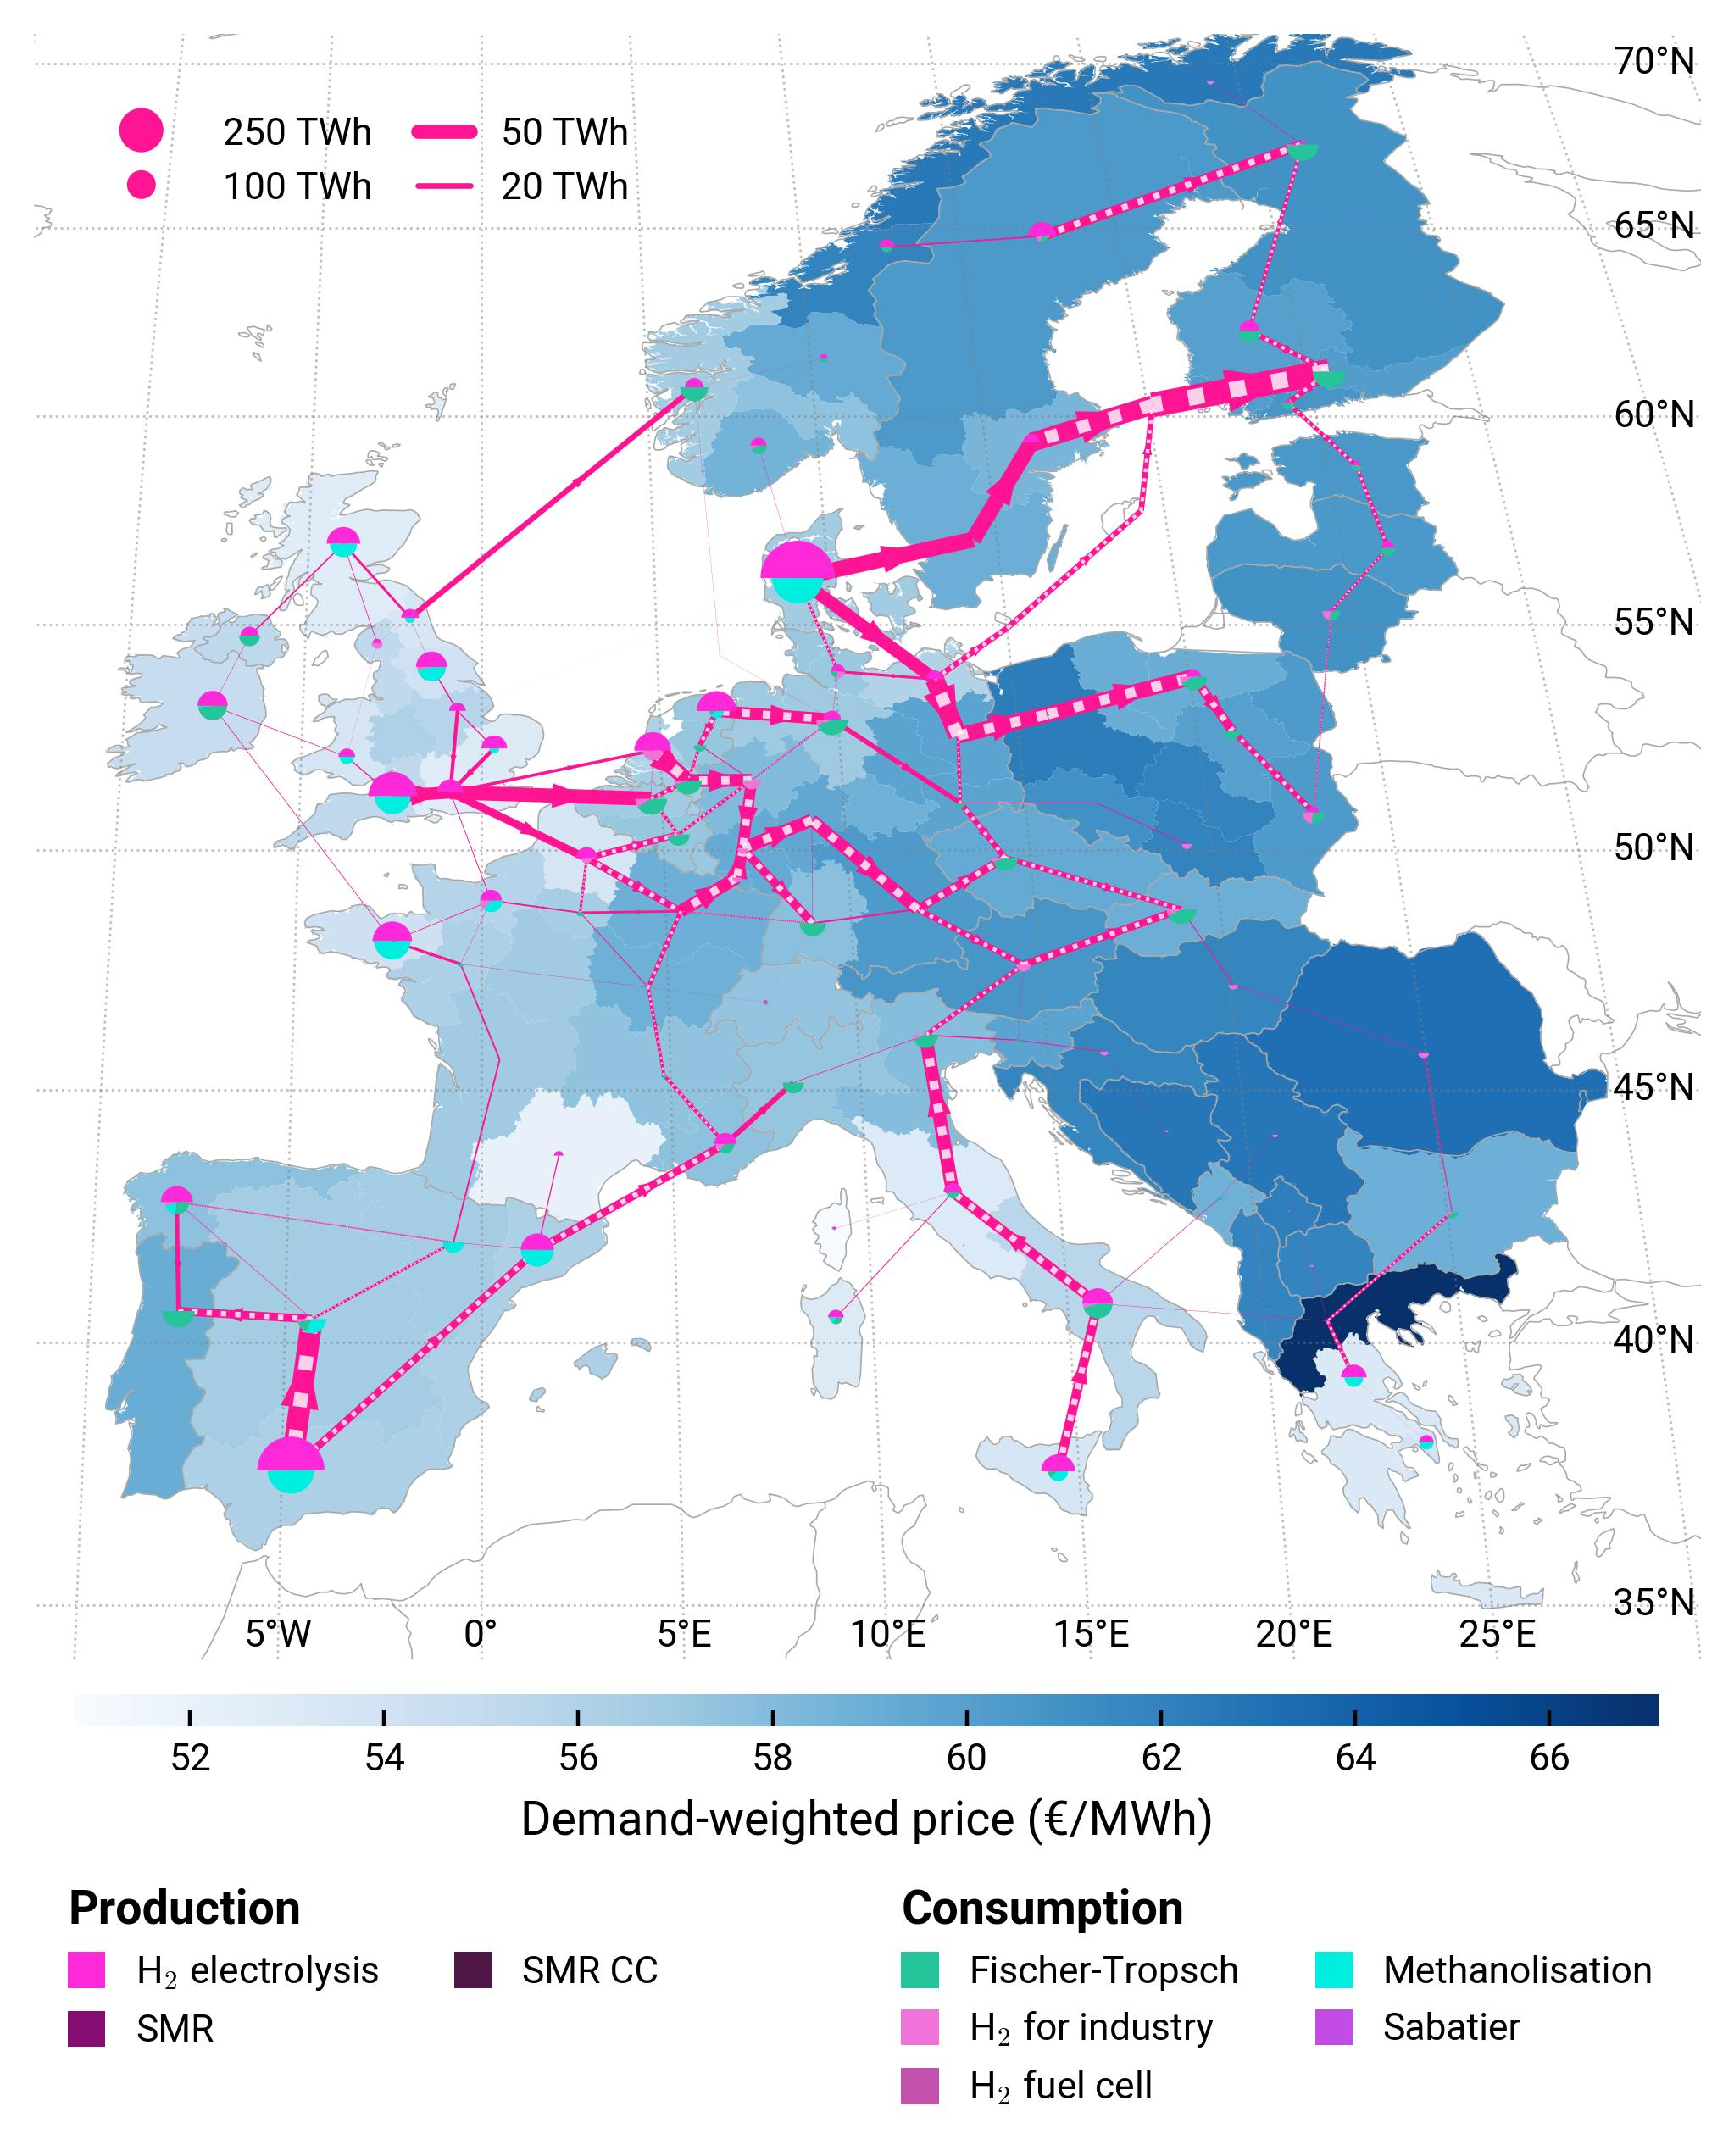
\includegraphics[width=1\textwidth]{maps/pcipmi-national-international-expansion/base_s_adm___2050-balance_map_H2}
    \caption{\ce{H2} 2050.}
    \label{fig:PCI-in_lt_2050_h2}
  \end{subfigure}
  \begin{subfigure}[t]{0.33\textwidth}
      \vspace{0pt}
      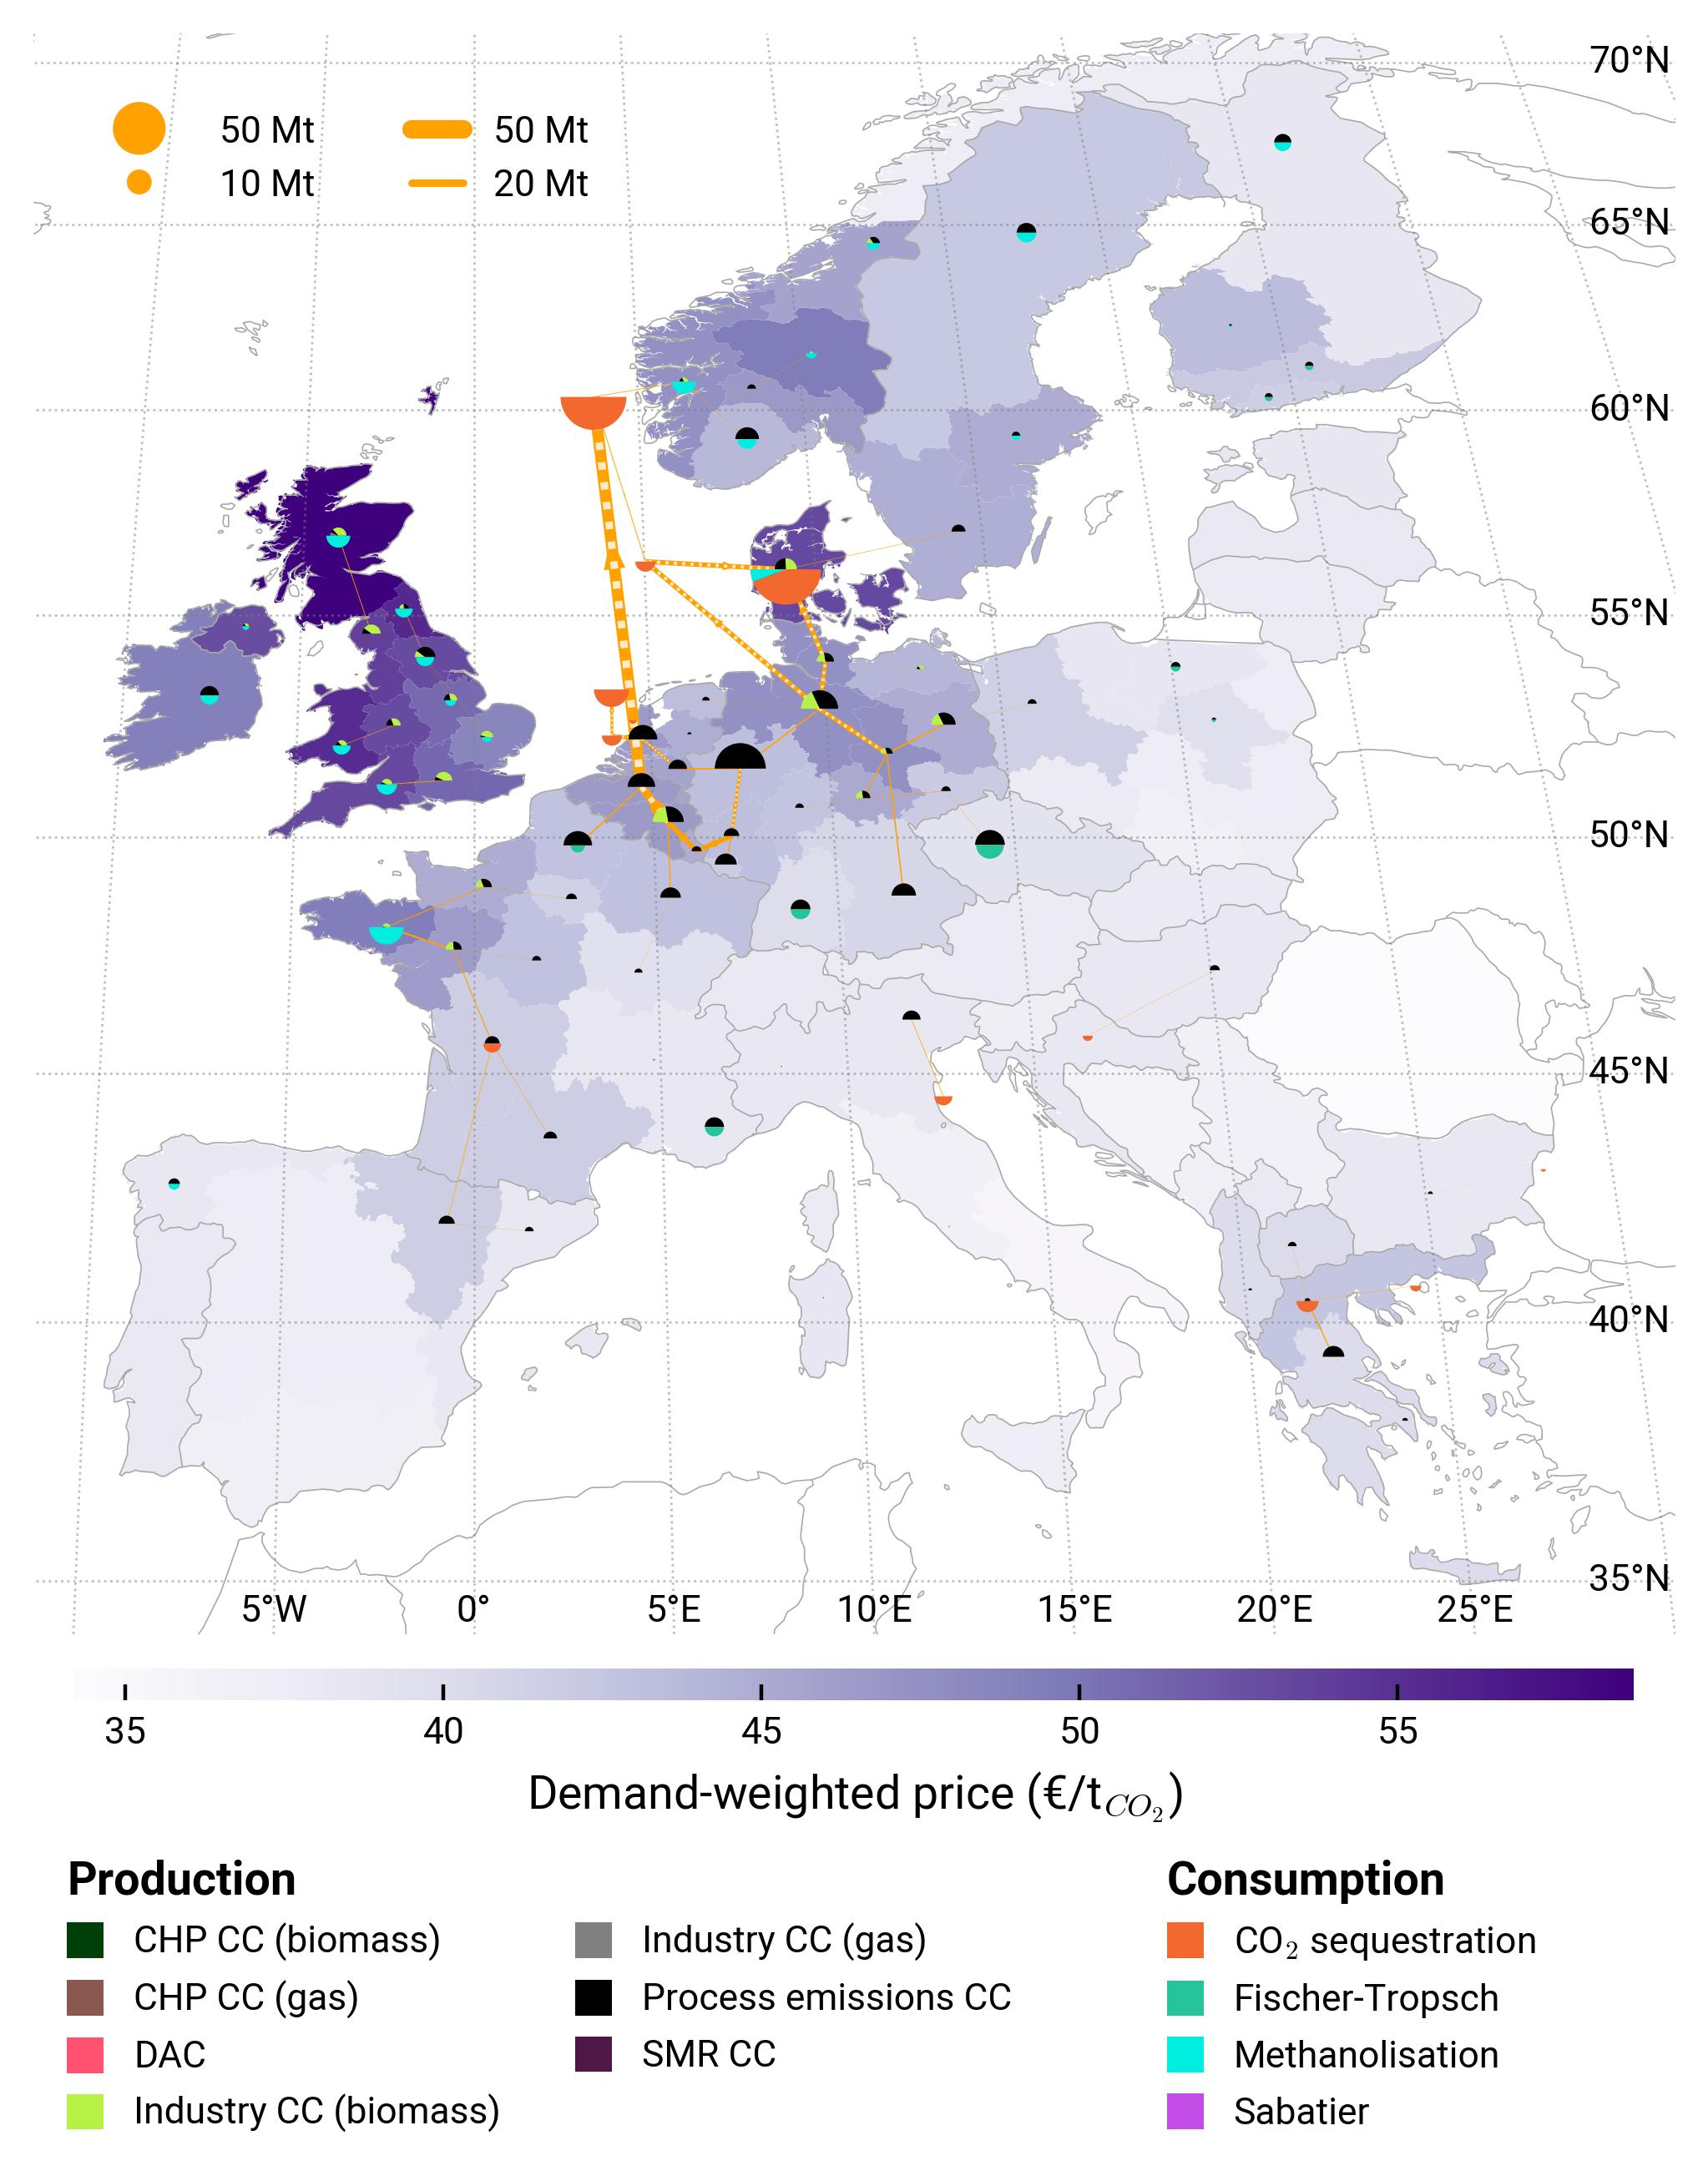
\includegraphics[width=1\textwidth]{maps/pcipmi-national-international-expansion/base_s_adm___2030-balance_map_co2_stored} 
      \caption{\ce{CO2} 2030.}
      \label{fig:PCI-in_lt_2030_co2}
  \end{subfigure}
  \begin{subfigure}[t]{0.33\textwidth}
      \vspace{0pt}
      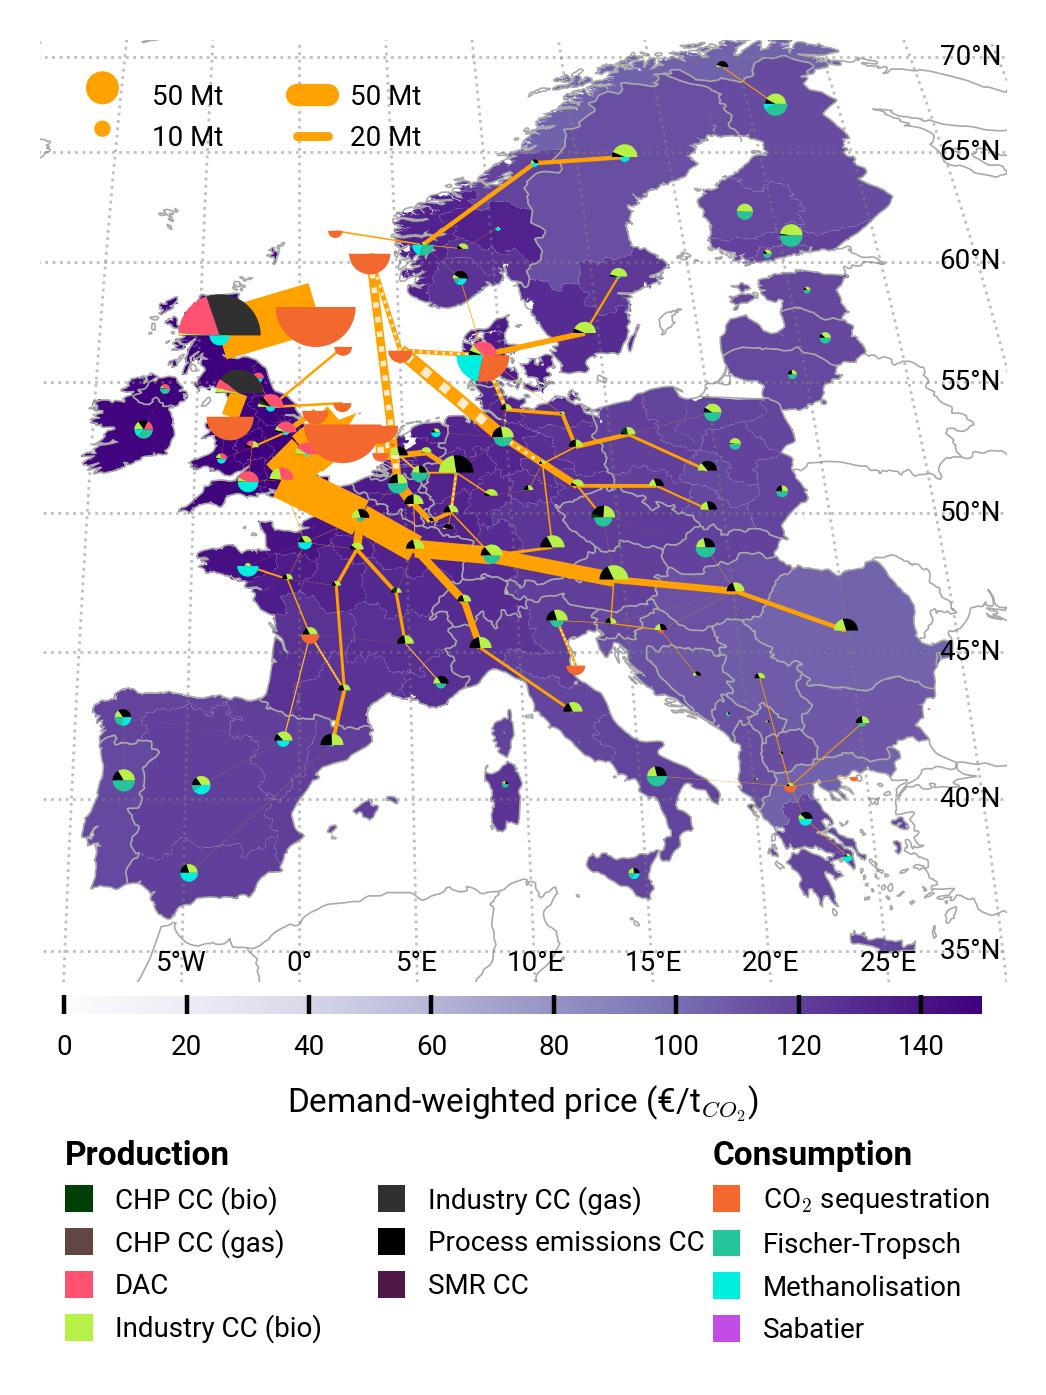
\includegraphics[width=1\textwidth]{maps/pcipmi-national-international-expansion/base_s_adm___2040-balance_map_co2_stored} 
      \caption{\ce{CO2} 2040.}
      \label{fig:PCI-in_lt_2040_co2}
  \end{subfigure}
  \begin{subfigure}[t]{0.33\textwidth}
      \vspace{0pt}
      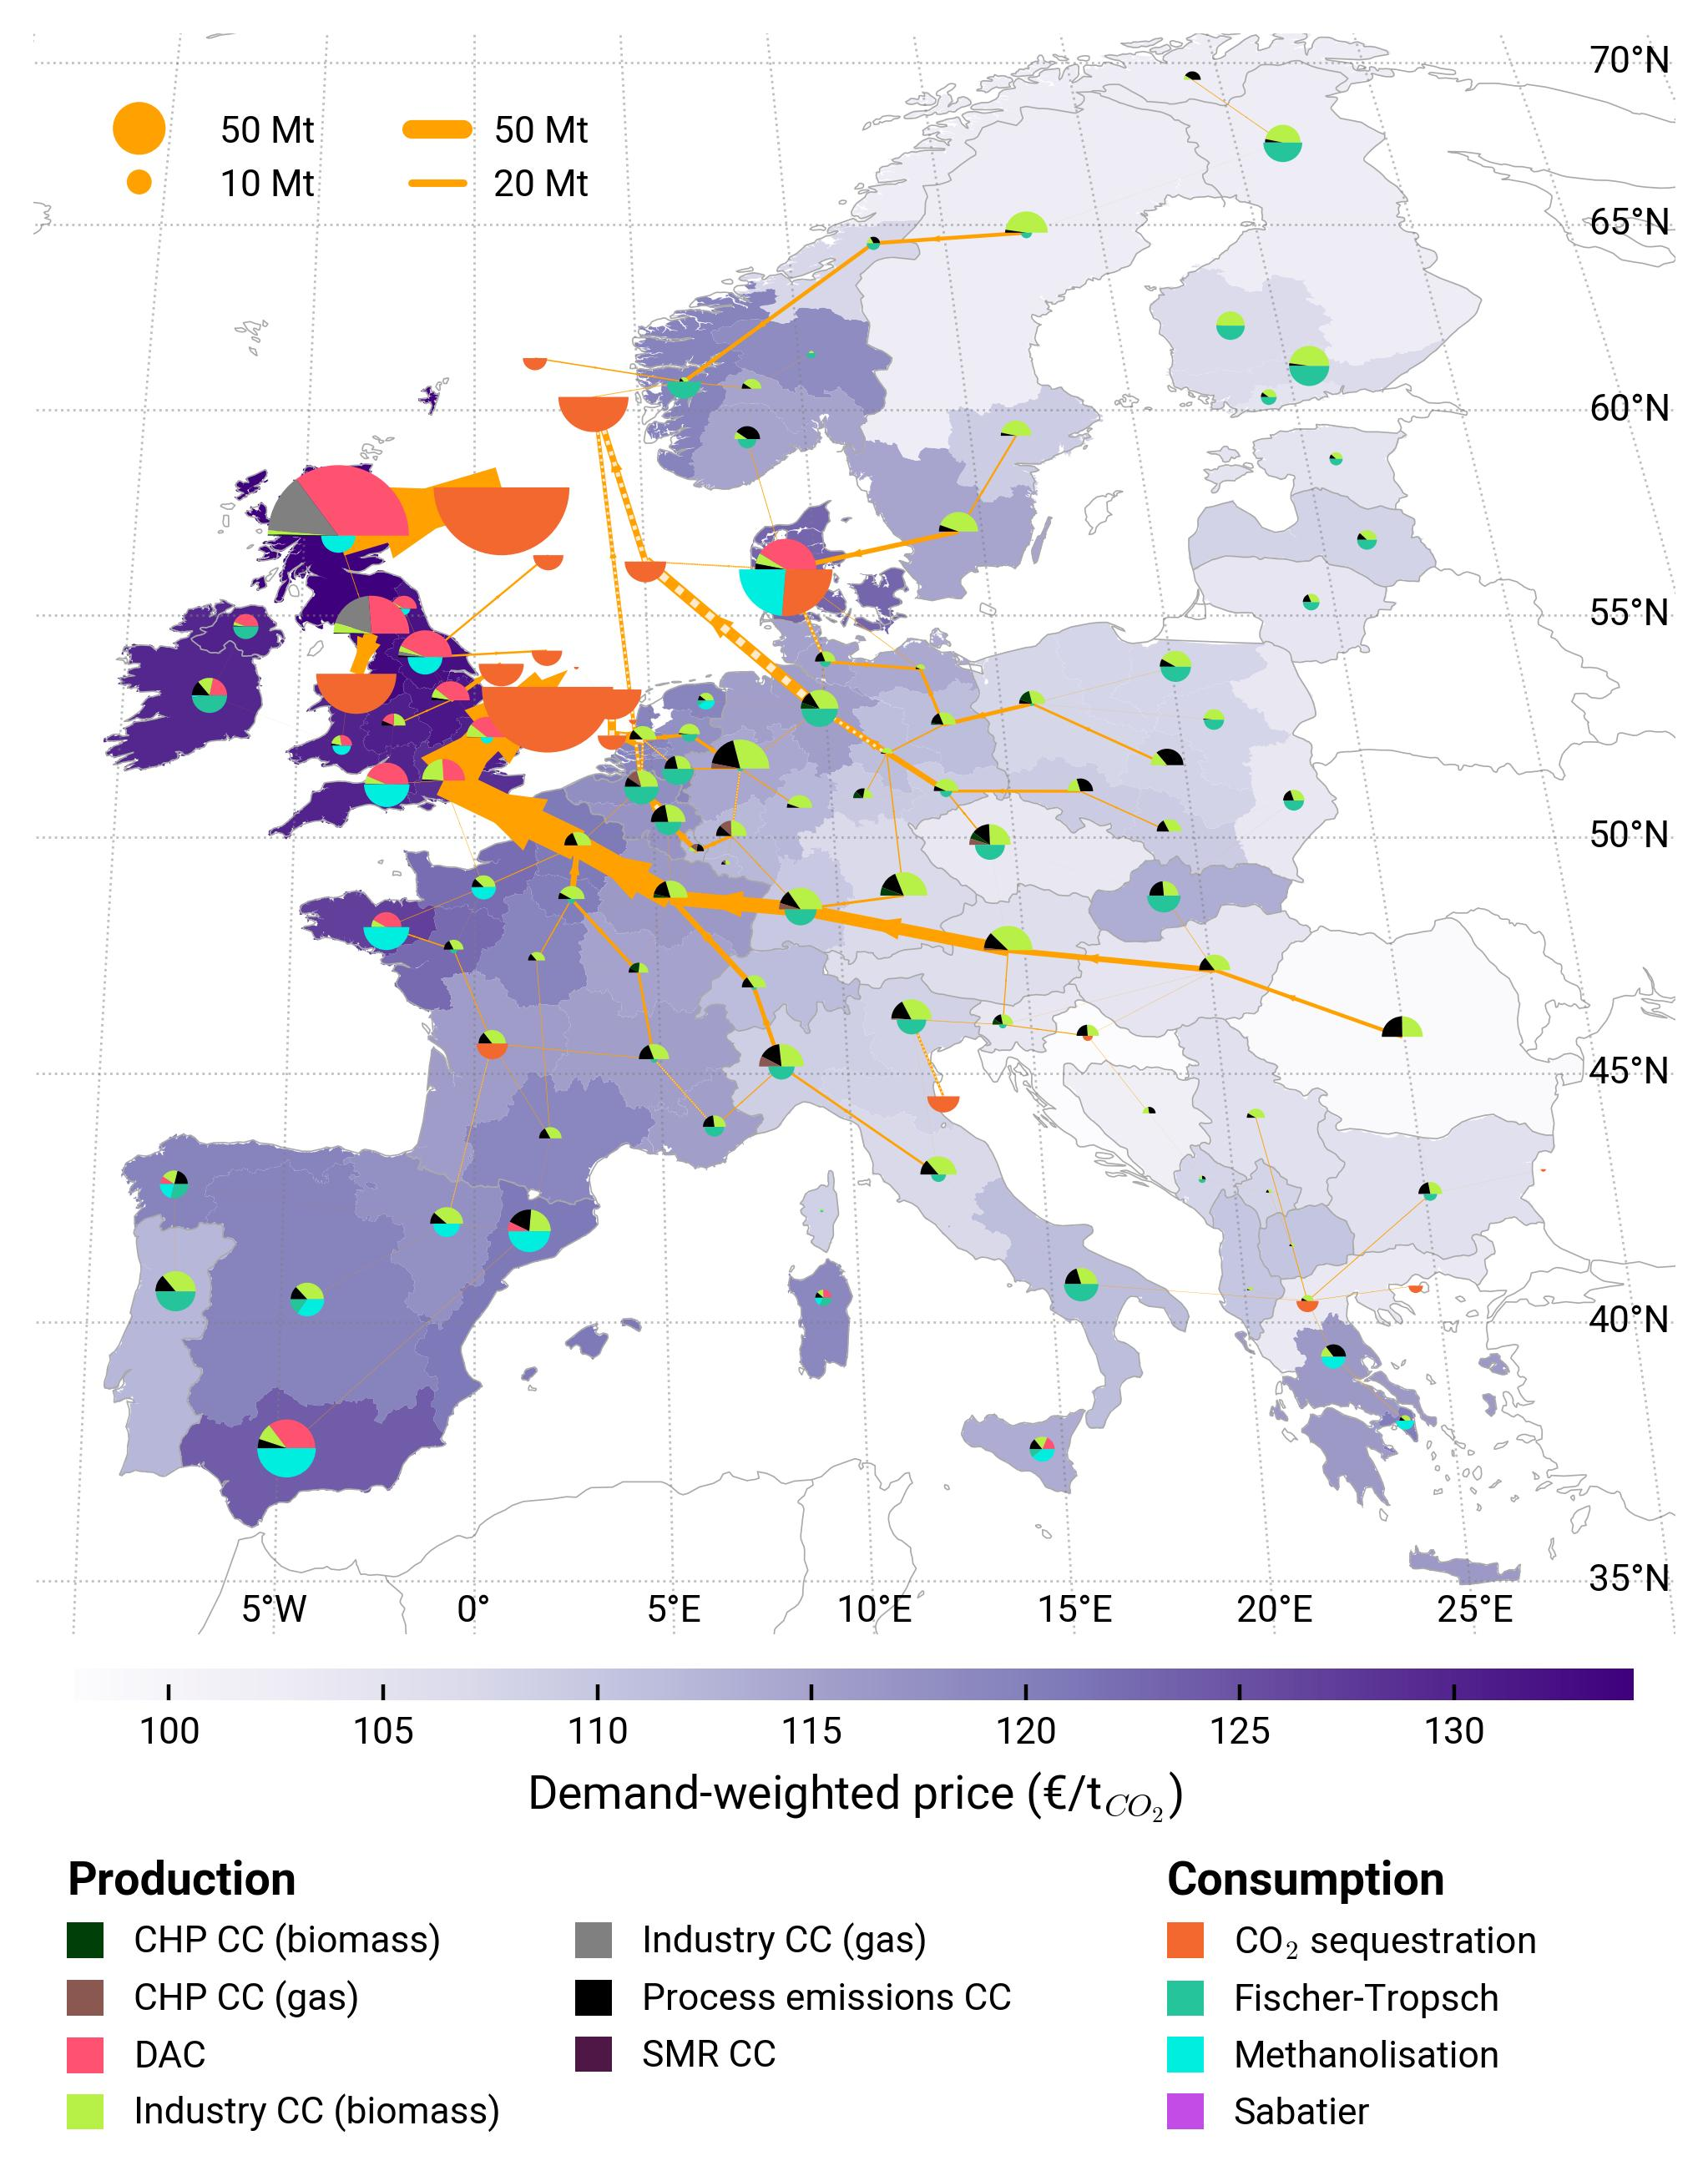
\includegraphics[width=1\textwidth]{maps/pcipmi-national-international-expansion/base_s_adm___2050-balance_map_co2_stored} 
      \caption{\ce{CO2} 2050.}
      \label{fig:PCI-in_lt_2050_co2}
  \end{subfigure}
  \vspace{0.3cm}
  \caption{\textit{PCI-PMI internat.} long-term scenario --- Regional distribution of \ce{H2} and \ce{CO2} production, utilisation, storage, transport and price. \textit{Note that both the \ce{H2} and \ce{CO2} price refer to their value as a commodity, i.e., price is higher where there is a demand for it.}}
  \label{fig:PCI-in_lt}
\end{figure*}


\begin{figure*}[htbp]
  \centering
  \begin{subfigure}[t]{0.33\textwidth}
      \vspace{0pt}
      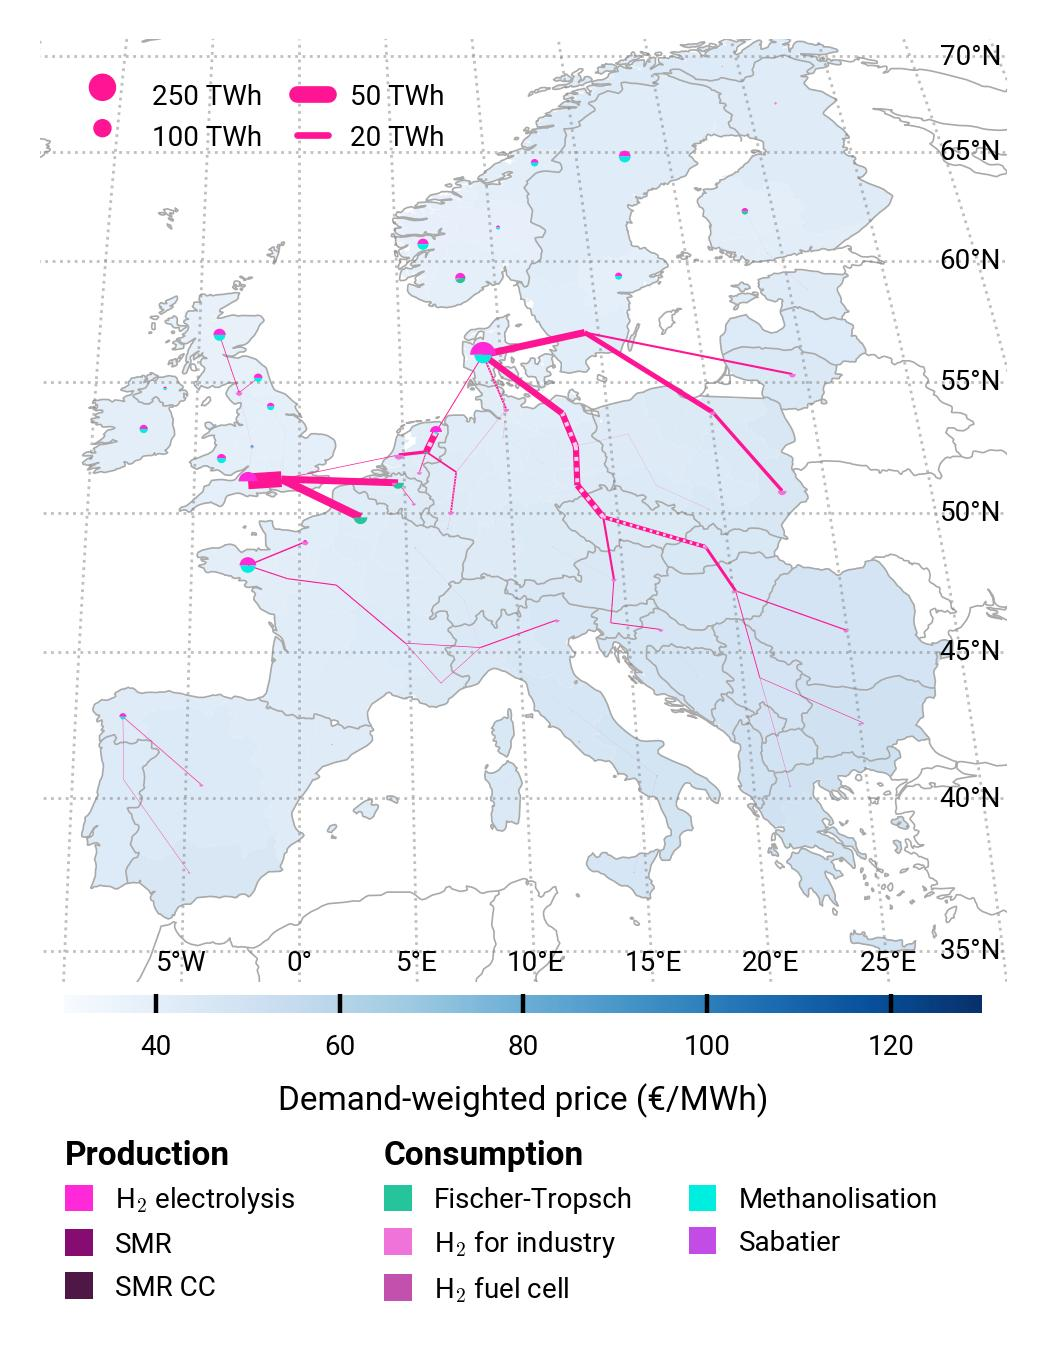
\includegraphics[width=1\textwidth]{maps/greenfield-pipelines/base_s_adm___2030-balance_map_H2}
      \caption{\ce{H2} 2030.}
      \label{fig:CP_lt_2030_h2}
  \end{subfigure}
  \begin{subfigure}[t]{0.33\textwidth}
      \vspace{0pt}
      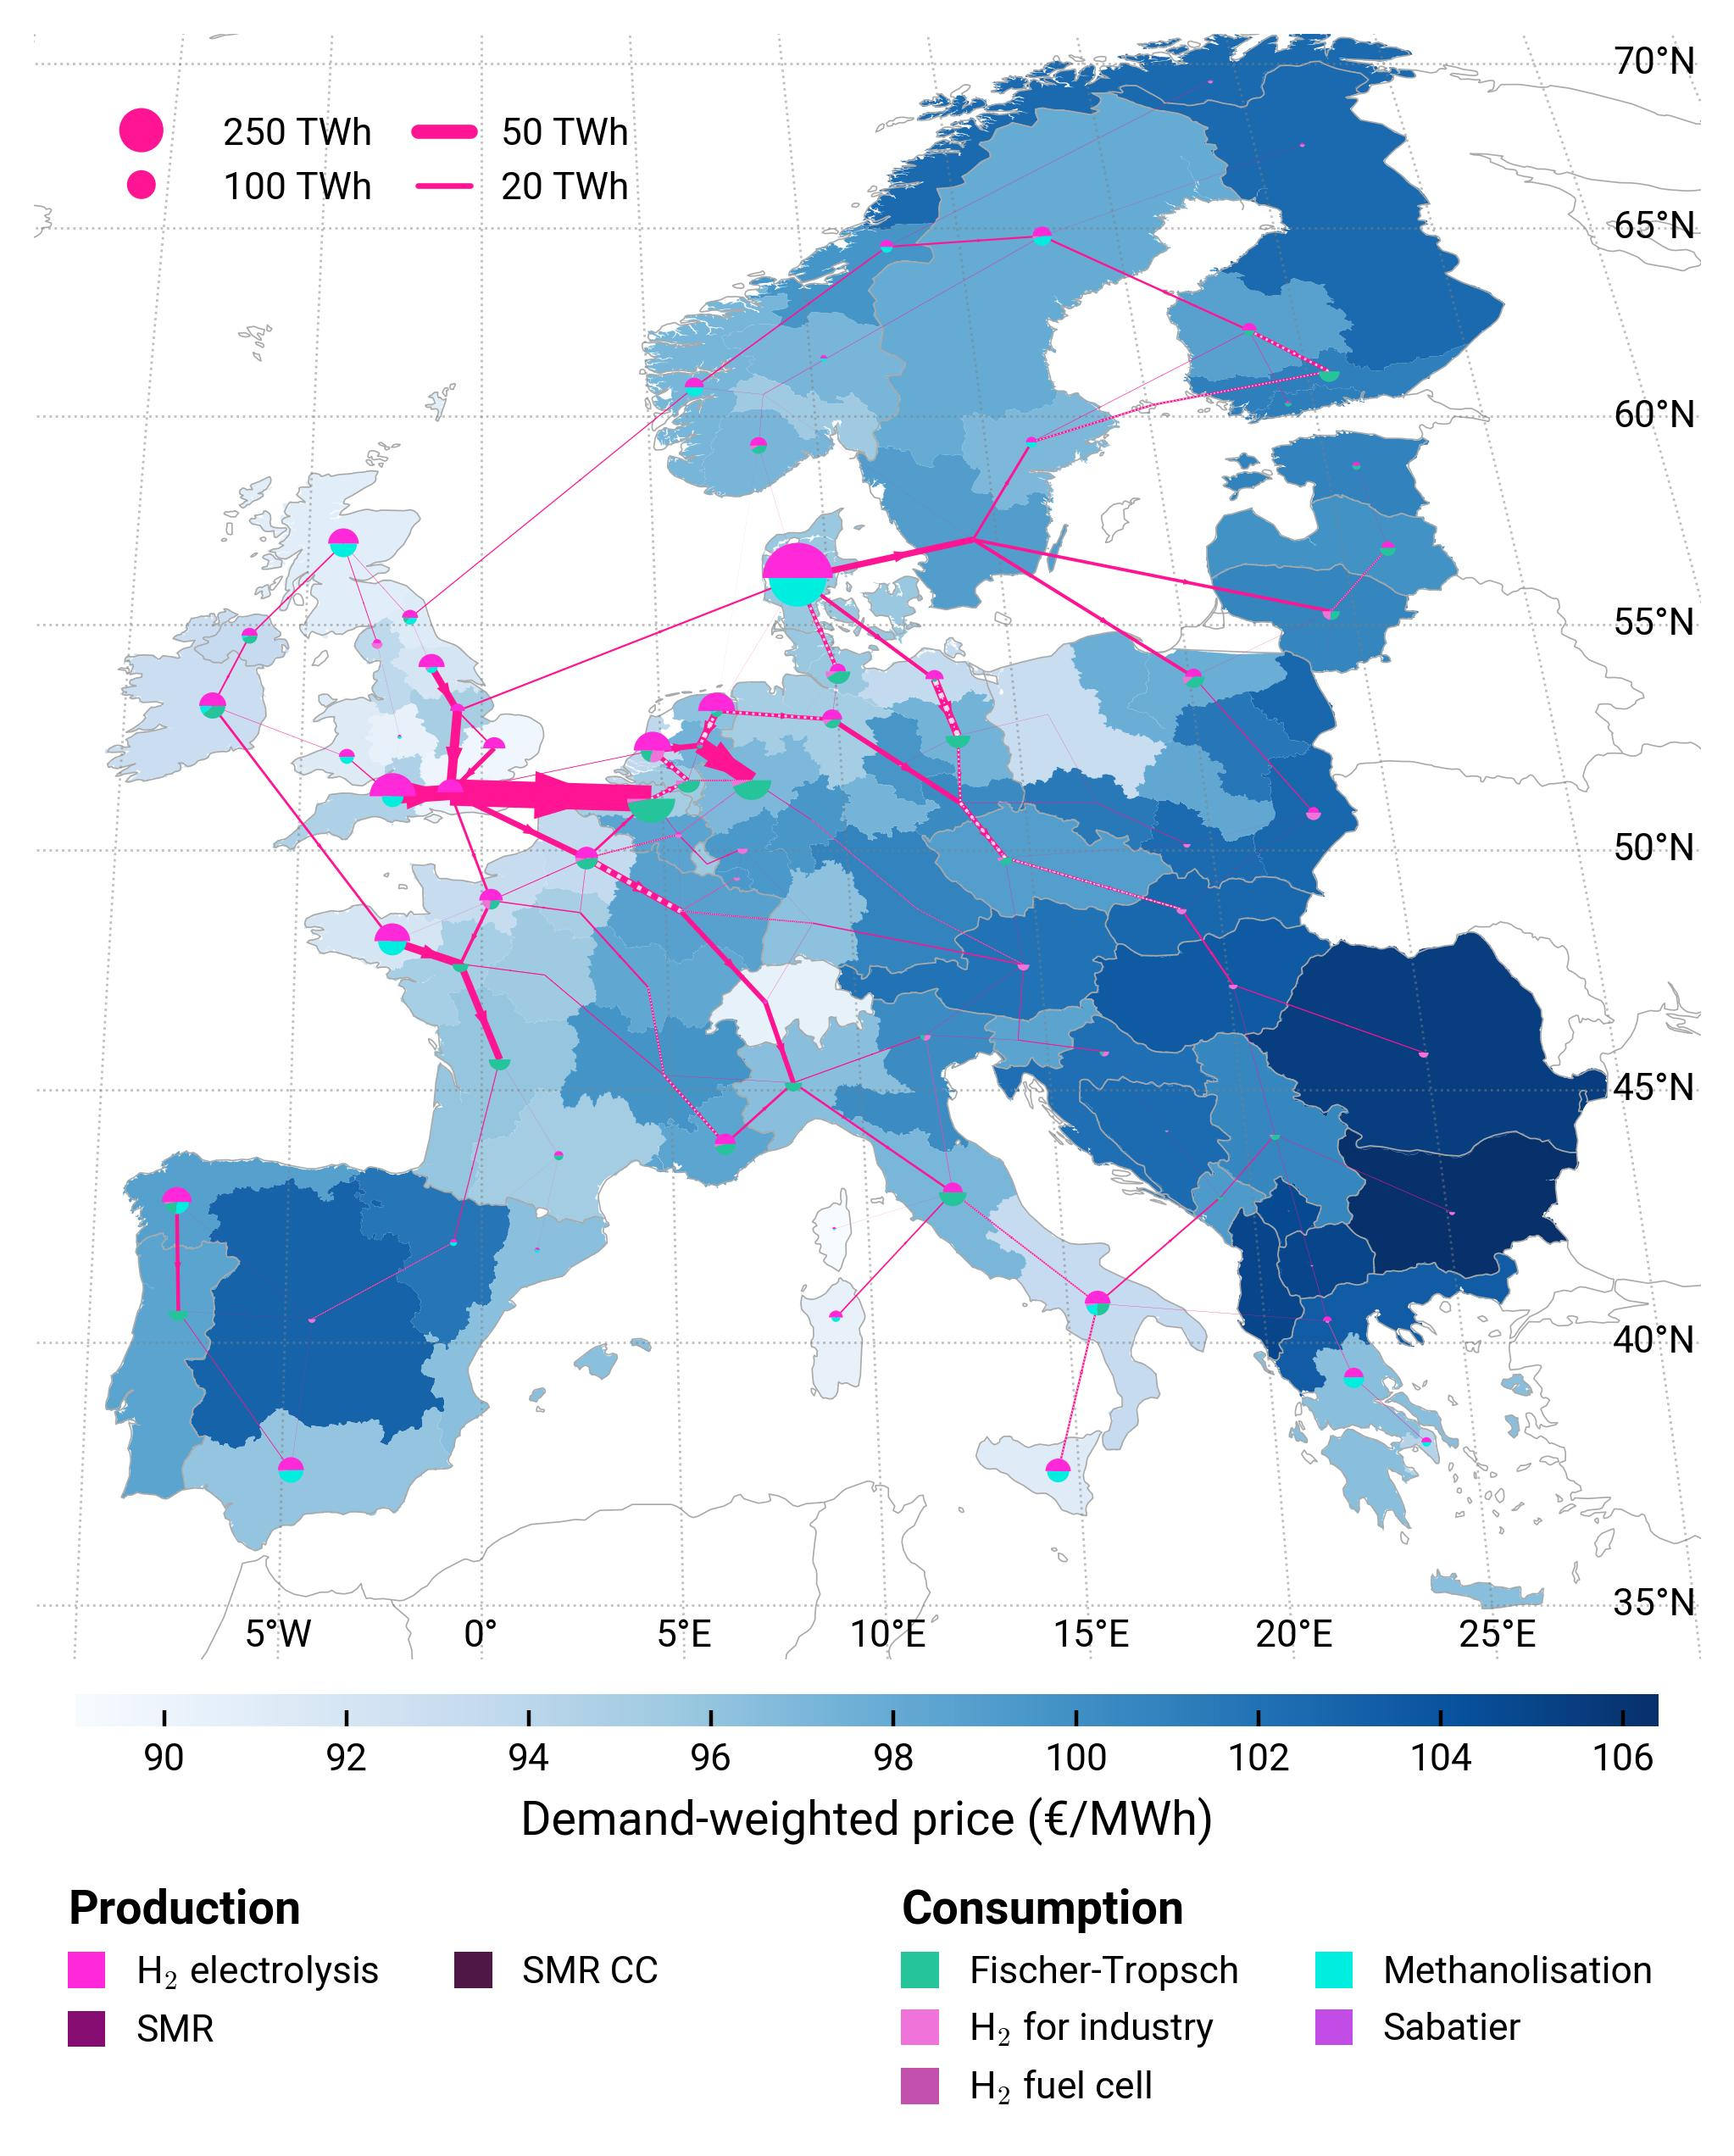
\includegraphics[width=1\textwidth]{maps/greenfield-pipelines/base_s_adm___2040-balance_map_H2}
      \caption{\ce{H2} 2040.}
      \label{fig:CP_lt_2040_h2}
  \end{subfigure}
  \begin{subfigure}[t]{0.33\textwidth}
    \vspace{0pt}
    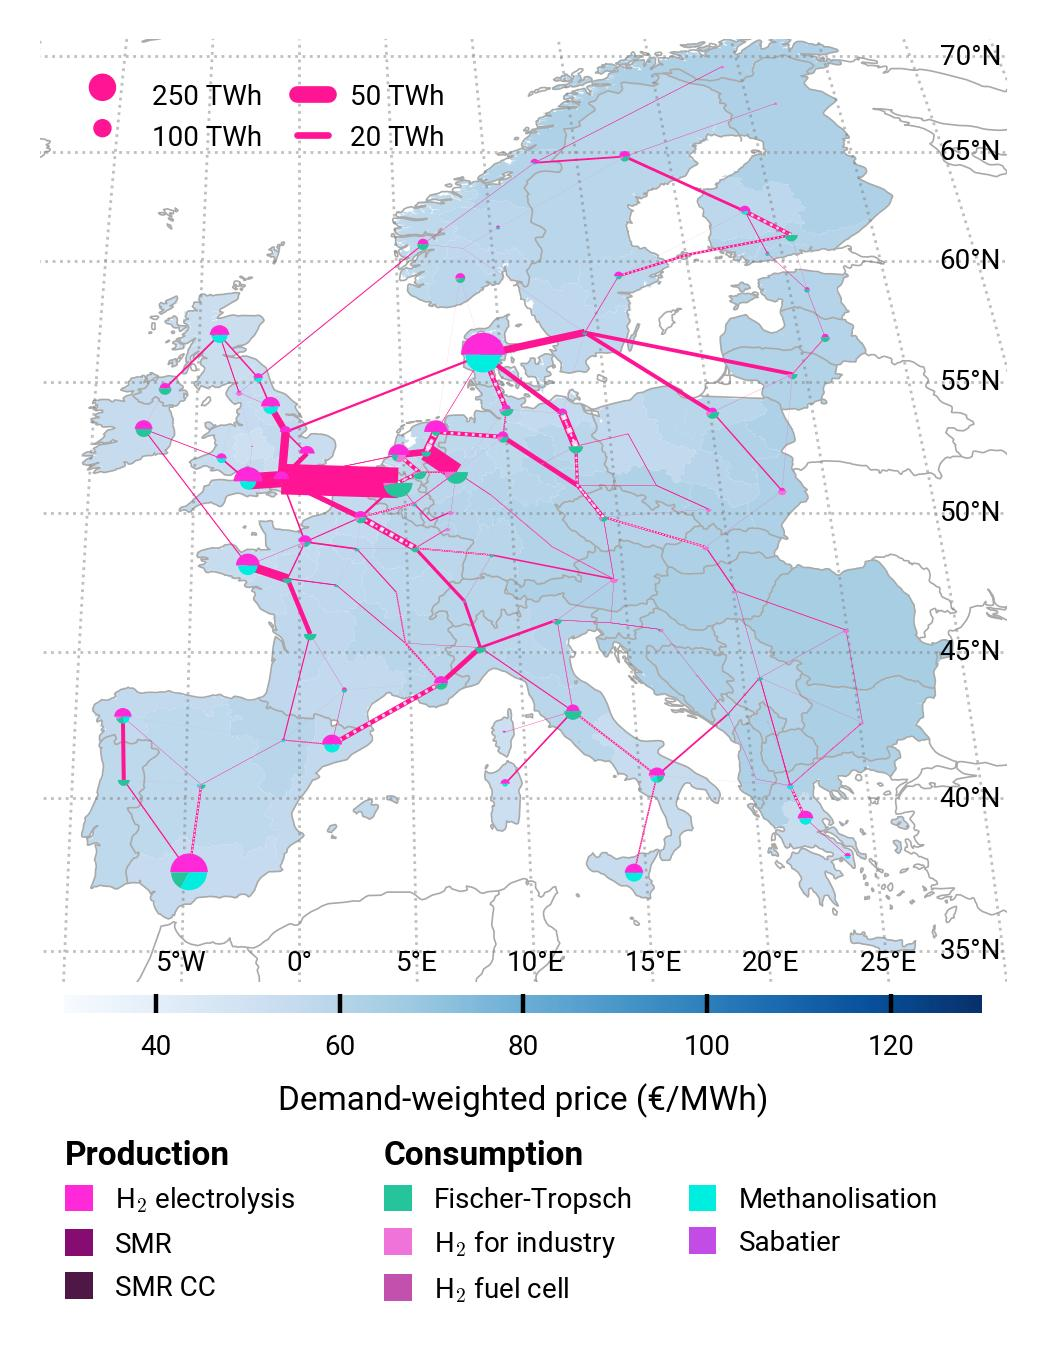
\includegraphics[width=1\textwidth]{maps/greenfield-pipelines/base_s_adm___2050-balance_map_H2}
    \caption{\ce{H2} 2050.}
    \label{fig:CP_lt_2050_h2}
  \end{subfigure}
  \begin{subfigure}[t]{0.33\textwidth}
      \vspace{0pt}
      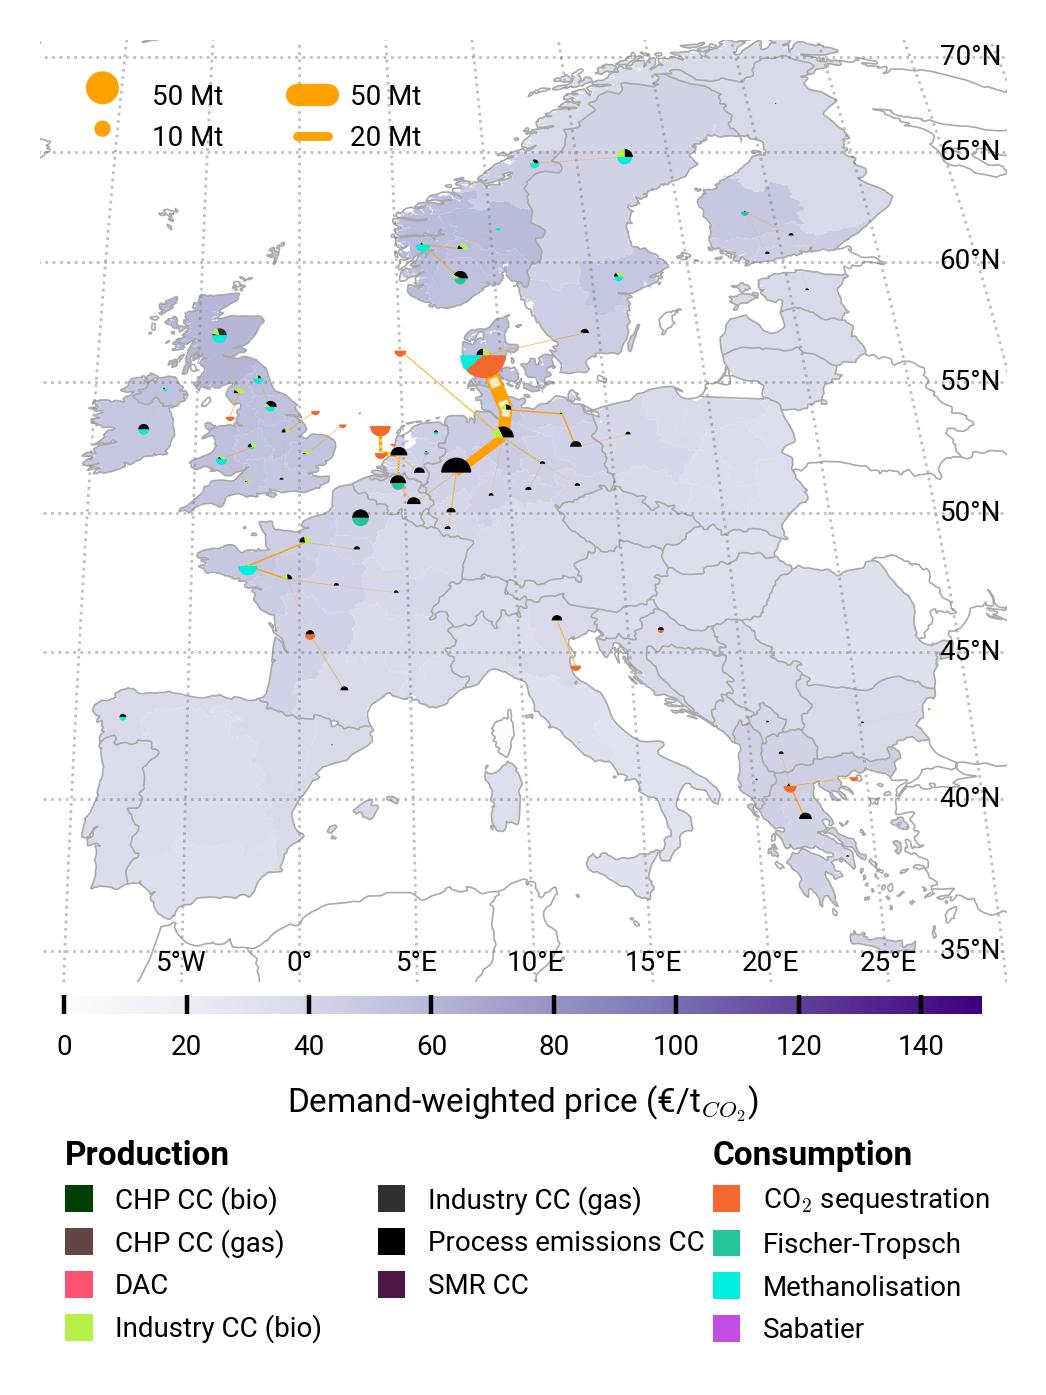
\includegraphics[width=1\textwidth]{maps/greenfield-pipelines/base_s_adm___2030-balance_map_co2_stored} 
      \caption{\ce{CO2} 2030.}
      \label{fig:CP_lt_2030_co2}
  \end{subfigure}
  \begin{subfigure}[t]{0.33\textwidth}
      \vspace{0pt}
      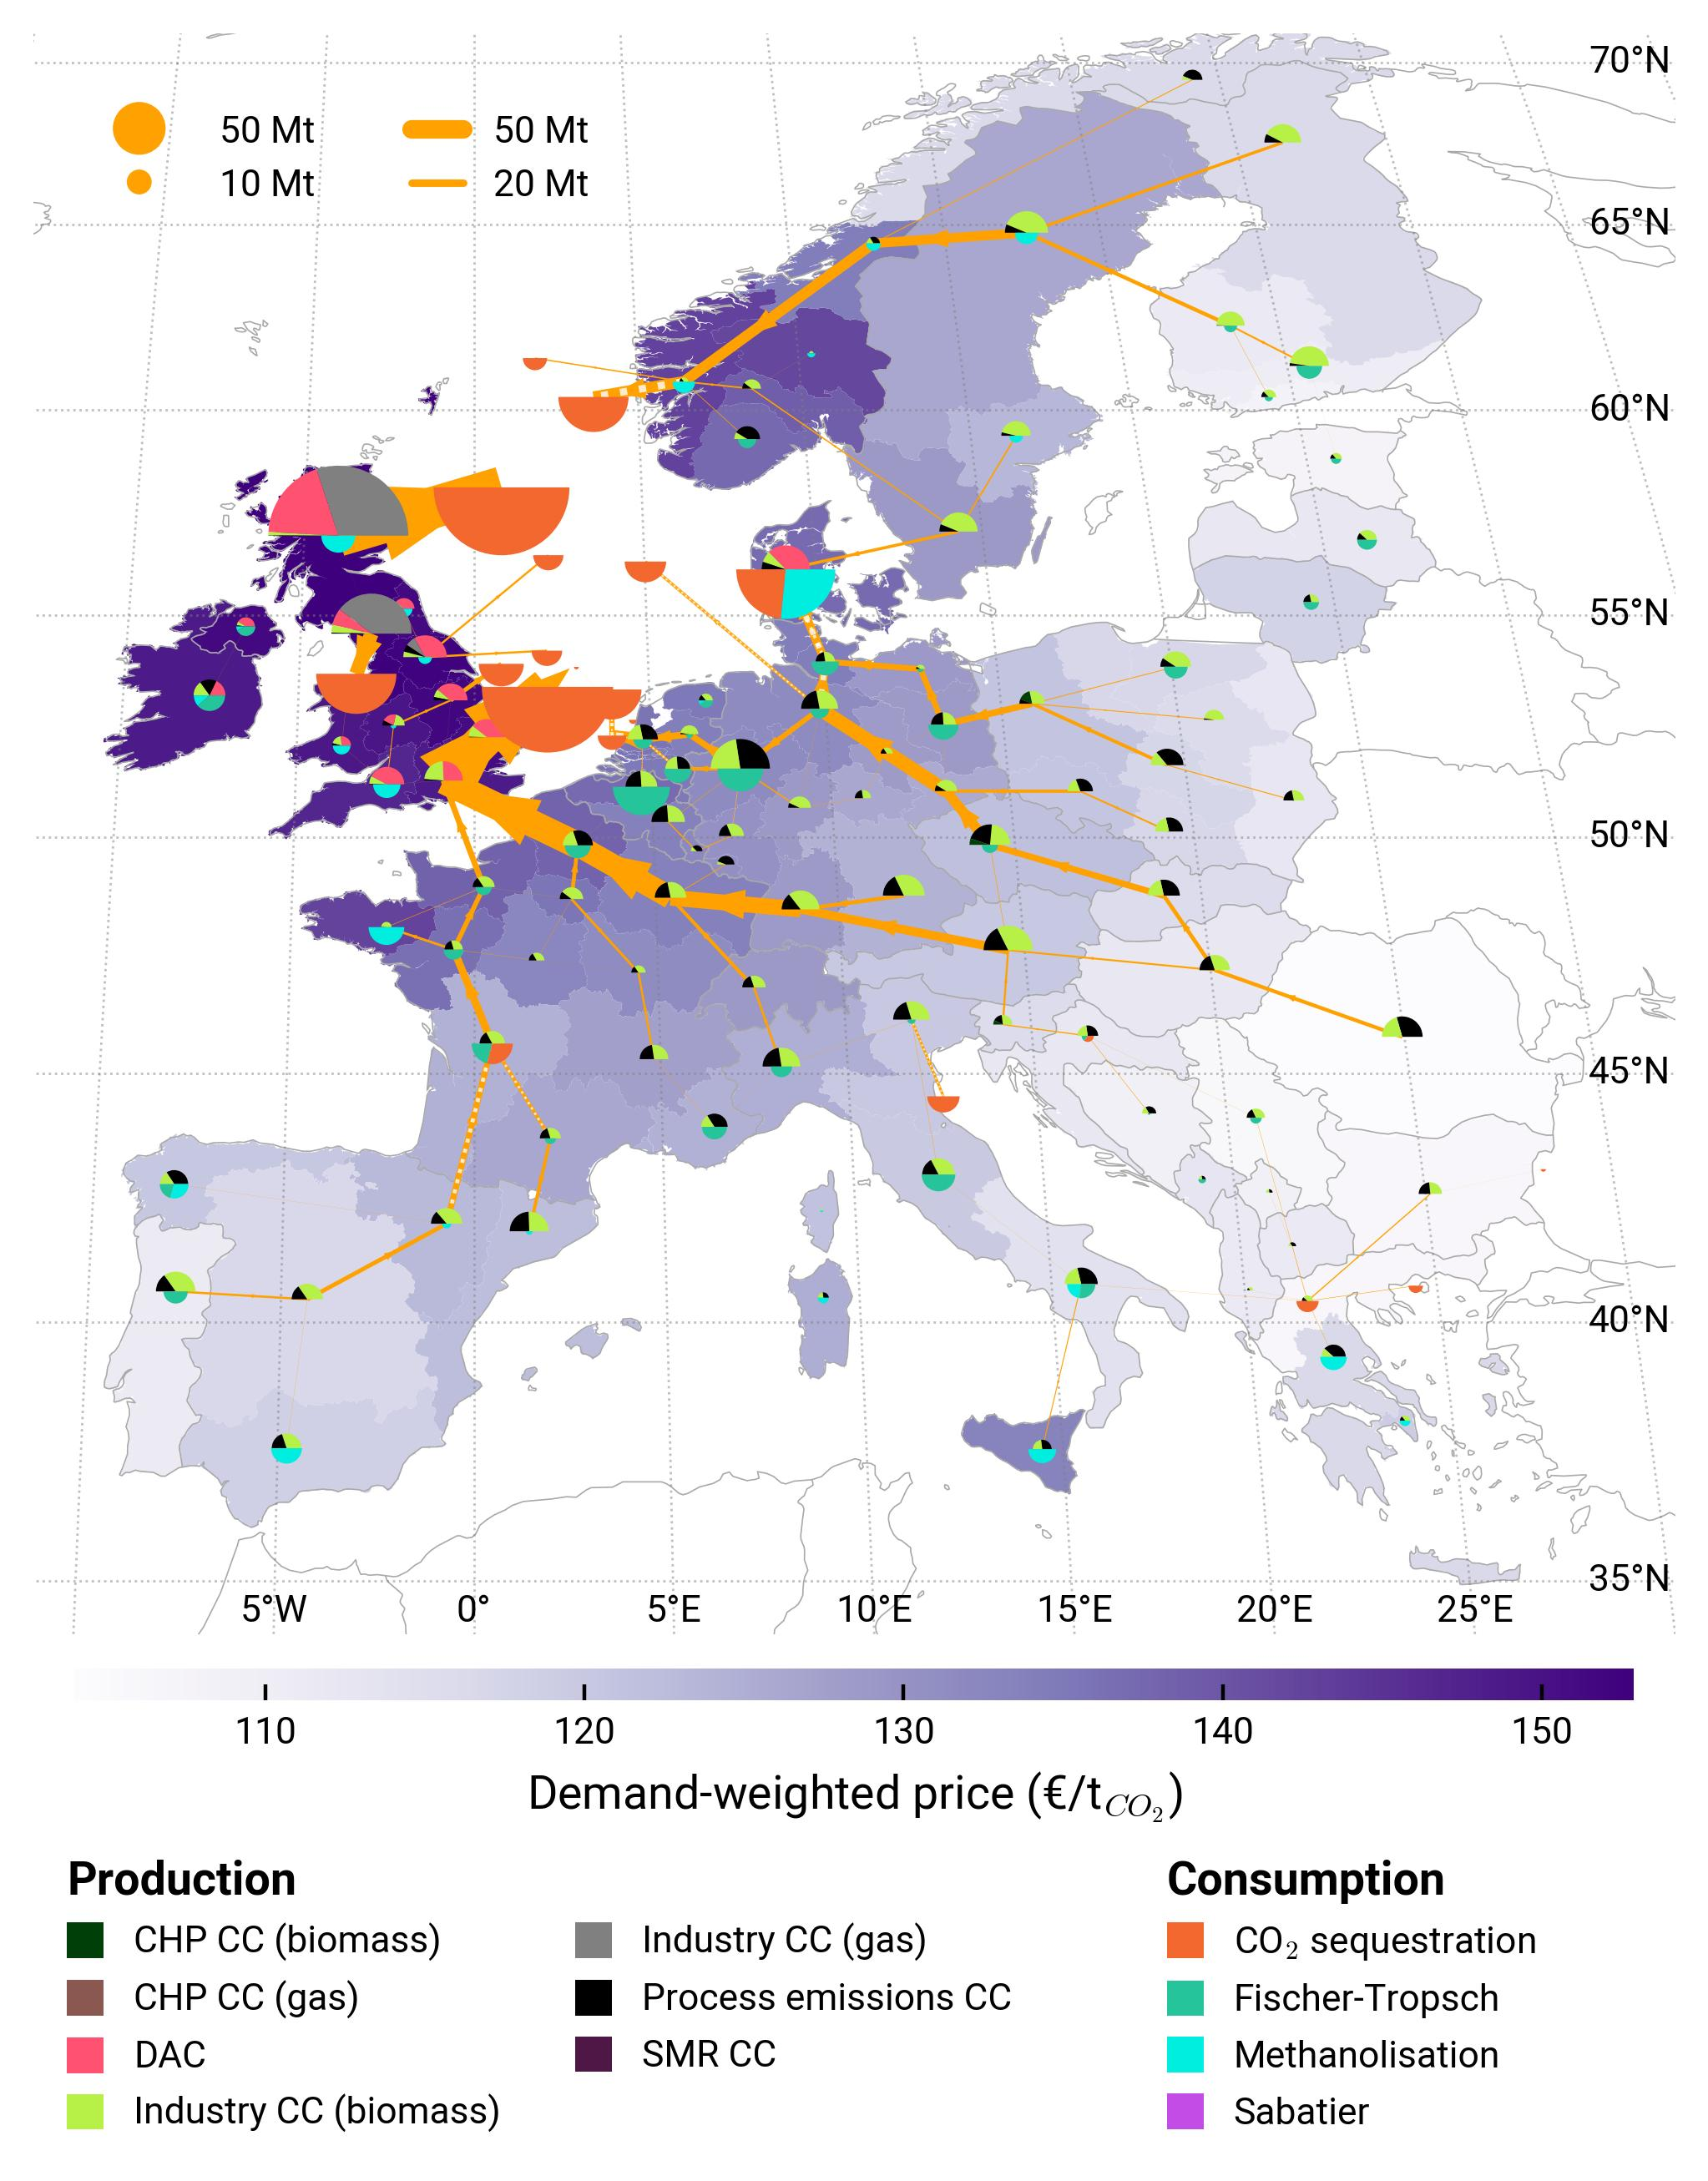
\includegraphics[width=1\textwidth]{maps/greenfield-pipelines/base_s_adm___2040-balance_map_co2_stored} 
      \caption{\ce{CO2} 2040.}
      \label{fig:CP_lt_2040_co2}
  \end{subfigure}
  \begin{subfigure}[t]{0.33\textwidth}
      \vspace{0pt}
      \includegraphics[width=1\textwidth]{maps/greenfield-pipelines/base_s_adm___2050-balance_map_co2_stored} 
      \caption{\ce{CO2} 2050.}
      \label{fig:CP_lt_2050_co2}
  \end{subfigure}
  \vspace{0.3cm}
  \caption{\textit{Central Planning} long-term scenario --- Regional distribution of \ce{H2} and \ce{CO2} production, utilisation, storage, transport and price. \textit{Note that both the \ce{H2} and \ce{CO2} price refer to their value as a commodity, i.e., price is higher where there is a demand for it.}}
  \label{fig:CP_lt}
\end{figure*}

\clearpage
\bibliographystyle{elsarticle-num} 
\bibliography{references.bib}

\end{document}

\endinput
%%
%% End of file `elsarticle-template-num.tex'.


%% Template related

% \section{Example Section}
% \label{sec1}
% %% Labels are used to cross-reference an item using \ref command.

% Section text. See Subsection \ref{subsec1}.

% %% Use \subsection commands to start a subsection.
% \subsection{Example Subsection}
% \label{subsec1}

% Subsection text.

% %% Use \subsubsection, \paragraph, \subparagraph commands to 
% %% start 3rd, 4th and 5th level sections.
% %% Refer following link for more details.
% %% https://en.wikibooks.org/wiki/LaTeX/Document_Structure#Sectioning_commands

% \subsubsection{Mathematics}
% %% Inline mathematics is tagged between $ symbols.
% This is an example for the symbol $\alpha$ tagged as inline mathematics.

% %% Displayed equations can be tagged using various environments. 
% %% Single line equations can be tagged using the equation environment.
% \begin{equation}
% f(x) = (x+a)(x+b)
% \end{equation}

% %% Unnumbered equations are tagged using starred versions of the environment.
% %% amsmath package needs to be loaded for the starred version of equation environment.
% \begin{equation*}
% f(x) = (x+a)(x+b)
% \end{equation*}

% %% align or eqnarray environments can be used for multi line equations.
% %% & is used to mark alignment points in equations.
% %% \\ is used to end a row in a multiline equation.
% \begin{align}
%  f(x) &= (x+a)(x+b) \\
%       &= x^2 + (a+b)x + ab
% \end{align}

% \begin{eqnarray}
%  f(x) &=& (x+a)(x+b) \nonumber\\ %% If equation numbering is not needed for a row use \nonumber.
%       &=& x^2 + (a+b)x + ab
% \end{eqnarray}

% %% Unnumbered versions of align and eqnarray
% \begin{align*}
%  f(x) &= (x+a)(x+b) \\
%       &= x^2 + (a+b)x + ab
% \end{align*}

% \begin{eqnarray*}
%  f(x)&=& (x+a)(x+b) \\
%      &=& x^2 + (a+b)x + ab
% \end{eqnarray*}

% %% Refer following link for more details.
% %% https://en.wikibooks.org/wiki/LaTeX/Mathematics
% %% https://en.wikibooks.org/wiki/LaTeX/Advanced_Mathematics

% %% Use a table environment to create tables.
% %% Refer following link for more details.
% %% https://en.wikibooks.org/wiki/LaTeX/Tables
% \begin{table}[t]%% placement specifier
% %% Use tabular environment to tag the tabular data.
% %% https://en.wikibooks.org/wiki/LaTeX/Tables#The_tabular_environment
% \centering%% For centre alignment of tabular.
% \begin{tabular}{l c r}%% Table column specifiers
% %% Tabular cells are separated by &
%   1 & 2 & 3 \\ %% A tabular row ends with \\
%   4 & 5 & 6 \\
%   7 & 8 & 9 \\
% \end{tabular}
% %% Use \caption command for table caption and label.
% \caption{Table Caption}\label{fig1}
% \end{table}


% %% Use figure environment to create figures
% %% Refer following link for more details.
% %% https://en.wikibooks.org/wiki/LaTeX/Floats,_Figures_and_Captions
% \begin{figure}[t]%% placement specifier
% %% Use \includegraphics command to insert graphic files. Place graphics files in 
% %% working directory.
% \centering%% For centre alignment of image.
% \includegraphics{example-image-a}
% %% Use \caption command for figure caption and label.
% \caption{Figure Caption}\label{fig1}
% %% https://en.wikibooks.org/wiki/LaTeX/Importing_Graphics#Importing_external_graphics
% \end{figure}

%% For citations use: 
%%       \cite{<label>} ==> [1]

%%
% Example citation, See \cite{lamport94}.

%% If you have bib database file and want bibtex to generate the
%% bibitems, please use

%% else use the following coding to input the bibitems directly in the
%% TeX file.

%% Refer following link for more details about bibliography and citations.
%% https://en.wikibooks.org/wiki/LaTeX/Bibliography_Management

% \begin{thebibliography}{00}

% %% For numbered reference style
% %% \bibitem{label}
% %% Text of bibliographic item

% \bibitem{lamport94}
%   Leslie Lamport,
%   \textit{\LaTeX: a document preparation system},
%   Addison Wesley, Massachusetts,
%   2nd edition,
%   1994.

% \end{thebibliography}